% 高一100_南洋中学_10月月考.tex
%   —— 高一上数学“2026-2027 年南洋中学高一上 10 月月考”（讲评版）
% 试卷版：xelatex 高一100_南洋中学_10月月考.tex
% 答案版：xelatex "\def\isanswer{1}% 高一100_南洋中学_10月月考.tex
%   —— 高一上数学“2026-2027 年南洋中学高一上 10 月月考”（讲评版）
% 试卷版：xelatex 高一100_南洋中学_10月月考.tex
% 答案版：xelatex "\def\isanswer{1}% 高一100_南洋中学_10月月考.tex
%   —— 高一上数学“2026-2027 年南洋中学高一上 10 月月考”（讲评版）
% 试卷版：xelatex 高一100_南洋中学_10月月考.tex
% 答案版：xelatex "\def\isanswer{1}% 高一100_南洋中学_10月月考.tex
%   —— 高一上数学“2026-2027 年南洋中学高一上 10 月月考”（讲评版）
% 试卷版：xelatex 高一100_南洋中学_10月月考.tex
% 答案版：xelatex "\def\isanswer{1}\input{高一100_南洋中学_10月月考.tex}"
% 紧凑版：xelatex "\def\iscompact{1}\input{高一100_南洋中学_10月月考.tex}"
%
% 原始材料：微信公众号“魔都数学加油站”文章，连载“27学年高一100”；
% 原文标题“27学年高一100——2026-2027年上海市南洋中学高一上10月月考”；
% 原文链接：https://mp.weixin.qq.com/s/uXLyt6VHraW4hSpDwnZDuQ。
% 正文为 10 张 PNG 页（`原图/高一100_南洋中学_10月月考/01..10.png`），
% 尺寸混排（第 2、4—9 页为 4762×6735，第 1、3、10 页为 2560×3620），按页序读取。
%
% 篇幅与题号：原卷自第 3 题起编号（第 1、2 题不在原文内）。填空题 3—12（10 题）、
% 选择题 13—16（4 题）、解答题 17—21（5 题），共 19 题。
%
% 讲评版：全部 19 题均印【解析】，其中第 13—16 题的答案在解析末句
% “故选 $C$／$B$／$D$／$B$”（题干括号内未印答案）。第 16 题解析带一幅
% 抛物线与 $y=2$ 的示意图，自原图裁切、去粉色水印后转灰度，三版都出。
%
% 副标题：原卷未印副标题。本稿按内容标作“集合与常用逻辑用语、不等式”。
%
% 原卷笔误/存疑（均照录未改，正文对应处另有 % 注）：无。
%
% 与原卷的排版差异：
%   ① 原卷每题下直接印【解析】，本稿按全稿惯例将答案与解析置于答案版；
%   ② 原卷未印副标题，本稿补出；填空横线统一排 \blankline[4.4em]；
%   ③ 原卷数集记号排斜体 $R$、$Z$、$\mathit N$，本稿按全稿惯例改用 $\R$、$\Z$、$\N$；
%   ④ 解答题按惯例加 \ansspace；选择题括号排 \mbox{（\quad）}；
%   ⑤ 第 16 题的示意图原卷排在解析行右侧，本稿改排为解析后的居中图。
%
% 行数核对：逐题数 \step/\stepm 条数，合计 117 条（Q3：2；Q4：5；Q5：7；Q6：3；Q7：3；
% Q8：4；Q9：2；Q10：4；Q11：6；Q12：3；Q13：7；Q14：3；Q15：5；Q16：3；Q17：5；
% Q18：11；Q19：9；Q20：10；Q21：25）。全卷 19 题均印【解析】。
% 原卷解析的换行按语意合并，未逐行强拆。
%
\documentclass[a4paper,11pt]{article}
\usepackage{common}
\begin{document}

\examtitlest[7]{2026--2027 年南洋中学高一上 10 月月考}{集合与常用逻辑用语、不等式}

\bigsec{一、填空题}

\begin{enumerate}
\setcounter{enumi}{2}

\item 不等式 $\dfrac{x-6}{x+1}\geqslant0$ 的解集为\blankline[4.4em].

\ifanswer
\solbegin
\step{不等式 $\dfrac{x-6}{x+1}\geqslant0$ 等价于 $\begin{cases}(x-6)(x+1)\geqslant0\\ x+1\neq0\end{cases}$，即 $x<-1$ 或 $x\geqslant6$，}
\step{故解集为 $(-\infty,-1)\cup[6,+\infty)$.}
\solend
\fi

\item 已知关于 $x$ 的不等式 $ax^2+bx+c>0$ 的解集是 $(1,3)$，则关于 $x$ 的不等式 $ax^2-bx+c\leqslant0$ 的解集为\blankline[4.4em].

\ifanswer
\solbegin
\step{由已知得 $a<0$，且 $1$，$3$ 是方程 $ax^2+bx+c=0$ 的根，}
\step{所以 $\begin{cases}1+3=-\dfrac ba\\[2pt] 1\times3=\dfrac ca\end{cases}$，所以 $\begin{cases}b=-4a\\ c=3a\end{cases}$，}
\step{所以 $ax^2-bx+c\leqslant0$ 可变形为 $ax^2+4ax+3a\leqslant0$，}
\step{因为 $a<0$，所以 $x^2+4x+3\geqslant0$，解得 $x\leqslant-3$ 或 $x\geqslant-1$，}
\step{所以不等式的解集为 $(-\infty,-3]\cup[-1,+\infty)$.}
\solend
\fi

\item 不等式 $\lvert x+2\rvert+\lvert 2x-1\rvert\geqslant3$ 的解集为\blankline[4.4em].

\ifanswer
\solbegin
\step{当 $x\leqslant-2$ 时，$x+2\leqslant0$，$2x-1<0$，}
\step{所以 $\lvert x+2\rvert+\lvert 2x-1\rvert=-x-2-2x+1\geqslant3$，解得 $x\leqslant-\dfrac43$；}
\step{当 $-2<x<\dfrac12$ 时，$x+2>0$，$2x-1<0$，}
\step{所以 $\lvert x+2\rvert+\lvert 2x-1\rvert=x+2-2x+1\geqslant3$，解得 $x\leqslant0$；}
\step{当 $x\geqslant\dfrac12$ 时，$x+2>0$，$2x-1\geqslant0$，}
\step{所以 $\lvert x+2\rvert+\lvert 2x-1\rvert=x+2+2x-1\geqslant3$，解得 $x\geqslant\dfrac23$；}
\step{所以原不等式的解集为 $\left\{x\mid x\leqslant0\right.$ 或 $\left.x\geqslant\dfrac23\right\}$.}
\solend
\fi

\item 若正数 $x$、$y$ 满足 $x+2y=2$，则 $\dfrac1x+\dfrac2y$ 的最小值是\blankline[4.4em].

\ifanswer
\solbegin
\step{因为 $x>0$，$y>0$，且 $x+2y=2$，}
\step{所以 $\dfrac1x+\dfrac2y=\dfrac12\left(\dfrac1x+\dfrac2y\right)(x+2y)=\dfrac12\left(5+\dfrac{2y}x+\dfrac{2x}y\right)\geqslant\dfrac12\left(5+2\sqrt{\dfrac{2y}x\cdot\dfrac{2x}y}\right)=\dfrac92$.}
\step{当且仅当 $\begin{cases}x+2y=2\\ \dfrac{2y}x=\dfrac{2x}y\end{cases}$，即 $x=y=\dfrac23$ 时取等号，故最小值为 $\dfrac92$.}
\solend
\fi

\item 已知 $\alpha:x\leqslant2$ 或 $x>3$，$\beta:x\leqslant m+5$ 或 $x>-m$，若 $\alpha$ 是 $\beta$ 的必要非充分条件，则实数 $m$ 的取值范围是\blankline[4.4em].

\ifanswer
\solbegin
\step{设 $A=\{x\mid x\leqslant2$ 或 $x>3\}$，$B=\{x\mid x\leqslant m+5$ 或 $x>-m\}$，则 $B\subset A$，}
\step{则 $m+5\leqslant2$ 且 $-m\geqslant3$（等号不能同时取得），则 $m<-3$，}
\step{则实数 $m$ 的取值范围是 $(-\infty,-3)$.}
\solend
\fi

\item 已知集合 $A=\{x\mid-1\leqslant x\leqslant3\}$，$B=\{x\mid ax+1>0\}$ 满足 $A\subseteq B$，则实数 $a$ 的取值范围为\blankline[4.4em].

\ifanswer
\solbegin
\step{当 $a=0$ 时，$B=R$，显然符合题意，}
\step{当 $a>0$ 时，$B=\left\{x\mid x>-\dfrac1a\right\}$，则 $-\dfrac1a<-1$，解得 $a<1$，所以 $0<a<1$，}
\step{当 $a<0$ 时，$B=\left\{x\mid x<-\dfrac1a\right\}$，则 $-\dfrac1a>3$，解得 $a>-\dfrac13$，所以 $-\dfrac13<a<0$，}
\step{综上所述，实数 $a$ 的取值范围为 $\left(-\dfrac13,1\right)$.}
\solend
\fi

\item 设集合 $A=\{x\mid3x-1<m\}$，若 $1\in A$ 且 $2\notin A$，则实数 $m$ 的取值范围是\blankline[4.4em].

\ifanswer
\solbegin
\step{因为集合 $A=\{x\mid3x-1<m\}$，若 $1\in A$ 且 $2\notin A$，}
\step{则 $3\times1-1<m$ 且 $3\times2-1\geqslant m$，解得 $2<m\leqslant5$.}
\solend
\fi

\item 若 $M=\left\{x\mid x=m+\dfrac16,m\in Z\right\},N=\left\{x\mid x=\dfrac n2-\dfrac13,n\in Z\right\}$，\newline $P=\left\{x\mid x=\dfrac p2+\dfrac16,p\in Z\right\}$，则 $M$、$N$、$P$ 的关系为\blankline[4.4em].

\ifanswer
\solbegin
\step{$M=\left\{x\mid x=m+\dfrac16=\dfrac{6m+1}6=\dfrac{3\cdot2m+1}6,m\in Z\right\}$，}
\step{$N=\left\{x\mid x=\dfrac n2-\dfrac13=\dfrac{3(n-1)+1}6,n\in Z\right\}=\left\{x\mid x=\dfrac{3k+1}6,k\in Z\right\}$，}
\step{$P=\left\{x\mid x=\dfrac p2+\dfrac16=\dfrac{3p+1}6,p\in Z\right\}$，}
\step{故 $M\subset N=P$.}
\solend
\fi

\item 已知命题 $p:x<-2$ 或 $x>3$，命题 $q:x<3m+1$ 或 $x>m+2$，若 $p$ 是 $q$ 的充分非必要条件，则实数 $m$ 的取值范围是\blankline[4.4em].

\ifanswer
\solbegin
\step{设 $A=\{x\mid x<-2$ 或 $x>3\}$，$B=\{x\mid x<3m+1$ 或 $x>m+2\}$，}
\step{若 $p$ 是 $q$ 的充分非必要条件，则 $A\subset B$，}
\step{当 $3m+1\geqslant m+2$，即 $m\geqslant\dfrac12$ 时，显然有 $A\subset B$，}
\step{当 $3m+1<m+2$，即 $m<\dfrac12$ 时，}
\step{由 $A\subset B$，则 $\begin{cases}m+2\leqslant3\\ 3m+1\geqslant-2\end{cases}$（等号不同时成立），即 $-1\leqslant m<\dfrac12$.}
\step{综上，实数 $m$ 的取值范围是 $[-1,+\infty)$.}
\solend
\fi

\item 对于一个有限集 $A$，一般都可以找到两个非空数集 $A_1$ 和 $A_2$，满足 $A_1\cap A_2=\varnothing$，且 $A_1\cup A_2=A$，记集合 $\{A_1,A_2\}$ 为 $A$ 的一个“划分集”．若 $A$ 中有 $n(n\geqslant2,n\in\N)$ 个元素，则不同的“划分集”共有\blankline[4.4em]个(用含 $n$ 的表达式填空).

\ifanswer
\solbegin
\step{集合中的每个元素都有属于 $A_1$ 或属于 $A_2$ 两种情况，故共有 $2^n$ 种情况，}
\step{排除全都属于 $A_1$ 或 $A_2$ 的两种情况，考虑对称情况，}
\step{故不同的“划分集”共有 $\dfrac12(2^n-2)=2^{n-1}-1$ 个.}
\solend
\fi

\end{enumerate}

\bigsec{二、选择题}

\begin{enumerate}
\setcounter{enumi}{12}

\item 下列命题中正确的\mbox{（\quad）}

\keepwithprev
A. $\varnothing$ 与 $\{0\}$ 表示同一个集合

B. 方程 $\{x\mid(x-2)^2(x-3)=0\}$ 的所有解的集合可表示为 $\{2,2,3\}$

C. 由 3，4，5 组成的集合可表示为 $\{3,4,5\}$ 或 $\{4,5,3\}$

D. 很小的实数可以构成集合.

\ifanswer
\solbegin
\step{对于 $A$，$\{0\}$ 中有一个元素 0，$\varnothing$ 中无任何元素，故 $\varnothing$ 与 $\{0\}$ 不是同一个集合，}
\step{故 $A$ 错误；}
\step{对于 $B$，$\{2,2,3\}$ 不满足集合元素的互异性，故 $B$ 错误；}
\step{对于 $C$，由集合的无序性，得由 3，4，5 组成的集合可表示为 $\{3,4,5\}$ 或 $\{4,5,3\}$，}
\step{故 $C$ 正确；}
\step{对于 $D$，由集合的确定性，很小的实数不能构成集合，故 $D$ 错误.}
\step{故选 $C$.}
\solend
\fi

\item 已知 $a\in R$，则“$\dfrac1a<1$”是“$a>1$”的\mbox{（\quad）}条件.

\keepwithprev
A. 充分非必要\qquad B. 必要非充分

C. 充要\qquad D. 既非充分又非必要

\ifanswer
\solbegin
\step{解 $\dfrac1a<1$，得 $a<0$ 或 $a>1$，}
\step{由 $a<0$ 或 $a>1$ 得不出 $a>1$，由 $a>1$ 得出 $a<0$ 或 $a>1$，}
\step{所以“$\dfrac1a<1$”是“$a>1$”的必要不充分条件．故选 $B$.}
\solend
\fi

\item 若命题“存在 $x_0\in R$ 使得 $ax_0^2+2ax_0+1\leqslant0$”是假命题，则实数 $a$ 的取值范围为\mbox{（\quad）}

\keepwithprev
A. $a<0$ 或 $a\geqslant1$\qquad B. $a\leqslant0$ 或 $a\geqslant1$\qquad C. $0<a<1$\qquad D. $0\leqslant a<1$

\ifanswer
\solbegin
\step{命题“存在 $x_0\in R$ 使得 $ax_0^2+2ax_0+1\leqslant0$”是假命题，}
\step{则 $\forall x\in R$，$ax^2+2ax+1>0$ 恒成立，}
\step{当 $a=0$ 时，满足题意，}
\step{当 $a\neq0$ 时，$\begin{cases}a>0\\ \Delta=4a^2-4a<0\end{cases}$，解得 $0<a<1$，}
\step{综上所述，实数 $a$ 的取值范围为 $\{a\mid0\leqslant a<1\}$．故选 $D$.}
\solend
\fi

\item 已知实数 $a<b$，关于 $x$ 的不等式 $x^2-(a+b)x+ab-2<0$ 的解集为 $(x_1,x_2)$，则实数 $a$、$b$、$x_1$、$x_2$ 从小到大的排列是\mbox{（\quad）}

\keepwithprev
A. $a<x_1<x_2<b$\qquad B. $x_1<a<b<x_2$\qquad C. $a<x_1<b<x_2$\qquad D. $x_1<a<x_2<b$

\ifanswer
\solbegin
\step{因为实数 $a<b$，不等式 $x^2-(a+b)x+ab-2<0$ 可化为 $(x-a)(x-b)<2$，}
\step{又其解集为 $(x_1,x_2)$，所以作出 $y=(x-a)(x-b)$ 与 $y=2$ 的图象如下：}
\begin{center}
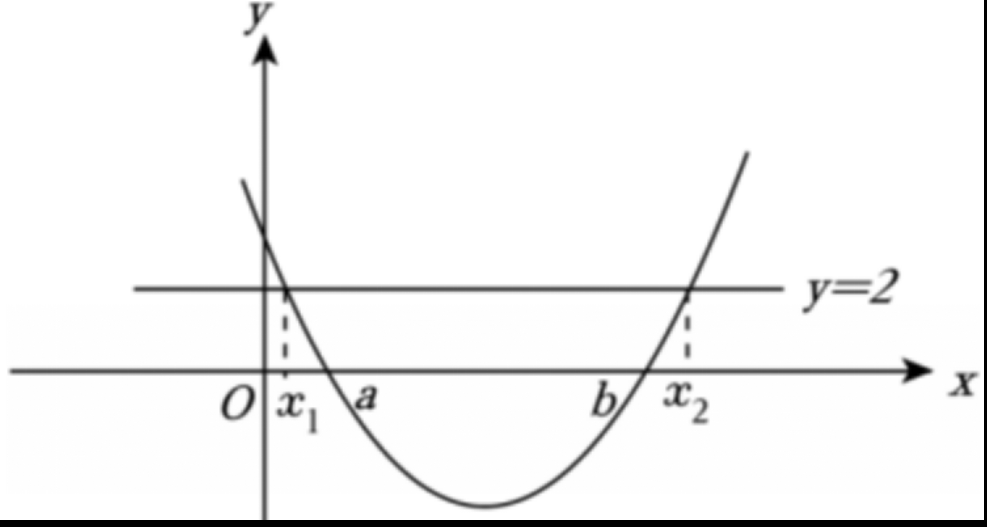
\includegraphics[width=0.42\textwidth]{figures/gao100_q16_parabola.png}
\end{center}
\step{所以数形结合得 $x_1<a<b<x_2$．故选 $B$.}
\solend
\fi

\end{enumerate}

\bigsec{三、解答题}

\begin{enumerate}
\setcounter{enumi}{16}

\item 已知集合 $A=\{x\mid3<x\leqslant6\}$，$B=\{x\mid m\leqslant x\leqslant2m+1\}$.

（1）若 $m=2$，求 $A\cap B$、$A\cup B$；

（2）若 $x\in B$ 是 $x\in A$ 的必要条件，求实数 $m$ 的取值范围.

\ansspace*[9]

\ifanswer
\solbegin
\stepm{（1）}{若 $m=2$，则 $B=\{x\mid2\leqslant x\leqslant5\}$，因为 $A=\{x\mid3<x\leqslant6\}$，}
\step{所以 $A\cap B=\{x\mid3<x\leqslant5\}$，$A\cup B=\{x\mid2\leqslant x\leqslant6\}$.}
\stepm{（2）}{因为 $x\in B$ 是 $x\in A$ 的必要条件，所以 $A\subseteq B$，}
\step{所以 $\begin{cases}m\leqslant3\\ 2m+1\geqslant6\end{cases}$，所以 $\dfrac52\leqslant m\leqslant3$，所以实数 $m$ 的取值范围为 $\left[\dfrac52,3\right]$.}
\solend
\fi

\item 求关于 $x$ 的不等式 $3ax^2-(3a+2)x+2<0\,(a\in R)$ 的解集.

\ansspace*[10]

\ifanswer
\solbegin
\step{当 $a=0$ 时，不等式化为 $-2x+2<0$，解得 $x>1$，}
\step{当 $a\neq0$ 时，方程 $3ax^2-(3a+2)x+2=0$ 的两根分别为 $1$，$\dfrac2{3a}$}
\step{当 $\dfrac2{3a}=1$，即 $a=\dfrac23$ 时，不等式化为 $(x-1)^2<0$，不等式无解，}
\step{当 $\dfrac2{3a}<1$，即 $a>\dfrac23$ 时，不等式解集为 $\left(\dfrac2{3a},1\right)$，}
\step{当 $0<a<\dfrac23$ 时，$\dfrac2{3a}>1$，不等式的解集为 $\left(1,\dfrac2{3a}\right)$，}
\step{当 $a<0$ 时，不等式的解集为 $\left(-\infty,\dfrac2{3a}\right)\cup(1,+\infty)$，}
\step{综上，当 $a=0$ 时，不等式的解集为 $(1,+\infty)$，}
\step{当 $a=\dfrac23$ 时，不等式的解集为 $\varnothing$，}
\step{当 $a>\dfrac23$ 时，不等式解集为 $\left(\dfrac2{3a},1\right)$，}
\step{当 $0<a<\dfrac23$ 时，不等式的解集为 $\left(1,\dfrac2{3a}\right)$，}
\step{当 $a<0$ 时，不等式的解集为 $\left(-\infty,\dfrac2{3a}\right)\cup(1,+\infty)$.}
\solend
\fi

\item 设对于任意实数 $x$，不等式 $\lvert x+1\rvert+\lvert x-1\rvert\geqslant m$ 恒成立.

（1）求 $m$ 的取值范围；

（2）当 $m$ 取最大值时，解关于 $x$ 的不等式 $\lvert x-3\rvert-2x\leqslant2m-2$.

\ansspace*[9]

\ifanswer
\solbegin
\stepm{（1）}{设函数 $f(x)=\lvert x+1\rvert+\lvert x-1\rvert$，则 $f(x)=\begin{cases}-2x,&x\leqslant-1\\ 2,&-1<x<1\\ 2x,&x\geqslant1\end{cases}$，}
\step{当 $x\leqslant-1$ 时，$f(x)$ 有最小值 2；}
\step{当 $-1<x<1$ 时，$f(x)=2$；}
\step{当 $x\geqslant1$ 时，$f(x)$ 有最小值 2；}
\step{因为对于任意实数 $x$，不等式 $\lvert x+1\rvert+\lvert x-1\rvert\geqslant m$ 恒成立，}
\step{所以 $m\leqslant2$，即 $m$ 的取值范围为 $(-\infty,2]$；}
\stepm{（2）}{由（1）得 $m$ 的最大值为 2，所以原不等式为 $\lvert x-3\rvert\leqslant2x+2$，}
\step{即 $-2x-2\leqslant x-3\leqslant2x+2$，解得 $x\geqslant\dfrac13$，}
\step{所以原不等式的解集为 $\left\{x\mid x\geqslant\dfrac13\right\}$.}
\solend
\fi

\item 某轮船公司的一艘轮船每小时花费的燃料费与轮船航行速度的平方成正比，比例系数为 $k$．轮船的最大速度为 18 海里/小时．当船速为 10 海里/小时，它的燃料费是每小时 120 元，其余航行运作费用（不论速度如何）总计是每小时 120 元．假定运行过程中轮船以速度 $v$ 匀速航行.

（1）求 $k$ 的值及每小时的最大总费用 $H$；

（2）求该轮船航行 100 海里的总费用 $W$（燃料费＋其余航行运作费用）的最小值.

\ansspace*[10]

\ifanswer
\solbegin
\stepm{（1）}{由题意，每小时燃料费为 $h(v)=kv^2$，$0<v\leqslant18$，}
\step{已知 $v=10$ 时，燃料费每小时 120 元，则 $k\cdot10^2=120$，得 $k=1.2$，}
\step{每小时总费用 $h(v)=kv^2+120=1.2v^2+120$，}
\step{$h(v)$ 是关于 $v$ 的增函数，$v$ 最大为 18，}
\step{所以 $H=h(18)=1.2\times18^2+120=508.8$ 元.}
\stepm{（2）}{航行时间 $t=\dfrac{100}v$ 小时，}
\step{$W(v)=h(v)\cdot t=(1.2v^2+120)\cdot\dfrac{100}v,0<v\leqslant18=120v+\dfrac{12000}v$，}
\step{利用均值不等式 $120v+\dfrac{12000}v\geqslant2\sqrt{120v\cdot\dfrac{12000}v}=2\times1200=2400$，}
\step{当且仅当 $120v=\dfrac{12000}v$，即 $v=10$ 时取等号，}
\step{$v=10\leqslant18$，在速度范围内，可取到等号，所以总费用最小值为 2400 元.}
\solend
\fi

\item 已知 $A$ 是 $R$ 的非空真子集，如果对任意 $x$、$y\in A$，都有 $x+y\in A$，$xy\in A$，则称 $A$ 是封闭集.

（1）判断集合 $B=\{0\}$，$C=\{-1,0,1\}$ 是否为封闭集，并说明理由；

（2）判断以下两个命题的真假，并说明理由；

命题 $p$：若非空集合 $A_1$、$A_2$ 是封闭集，则 $A_1\cup A_2$ 也是封闭集；

命题 $q$：非空集合 $A_1$、$A_2$ 是封闭集，则 $A_1\cap A_2\neq\varnothing$ 是 $A_1\cap A_2$ 是封闭集的充要条件；

（3）若非空集合 $A$ 是封闭集合，设全集为 $R$，求证：$A$ 的补集不是封闭集.

\ansspace*[13]

\ifanswer
\solbegin
\stepm{（1）}{$B=\{0\}$ 是封闭集，$C=\{-1,0,1\}$ 不是封闭集，理由如下：}
\step{对于集合 $B=\{0\}$，因为 $0+0=0\in B$，$0\times0=0\in B$，}
\step{所以 $B=\{0\}$ 是封闭集；}
\step{对于集合 $C=\{-1,0,1\}$，因为 $-1+(-1)=-2\notin C$，$1+1=2\notin C$，}
\step{所以集合 $C=\{-1,0,1\}$ 不是封闭集.}
\stepm{（2）}{命题 $p$ 是假命题，命题 $q$ 是真命题，理由如下：}
\step{对命题 $p$：令 $A_1=\{x\mid x=2k,k\in Z\}$，$A_2=\{x\mid x=3k,k\in Z\}$，}
\step{令 $x_1=2k_1$，$y_1=2k_2$，$k_1$、$k_2\in Z$，}
\step{则 $x_1+y_1=2(k_1+k_2)\in A_1$，$x_1y_1=2(2k_1k_2)\in A_1$，}
\step{因此集合 $A_1$ 是封闭集，同理集合 $A_2$ 也是封闭集，}
\step{取 $x_2=2$，$y_2=3$，则 $x_2$、$y_2\in(A_1\cup A_2)$，而 $x_2+y_2=5\notin(A_1\cup A_2)$，}
\step{因此集合 $A_1\cup A_2$ 不是封闭集，命题 $p$ 是假命题；}
\step{对于命题 $q$：若 $A_1\cap A_2\neq\varnothing$，不妨令 $a$、$b\in(A_1\cap A_2)$，}
\step{则有 $a$、$b\in A_1$，又集合 $A_1$ 是封闭集，则 $a+b\in A_1$，$ab\in A_1$，}
\step{同理 $a+b\in A_2$，$ab\in A_2$，因此 $a+b\in(A_1\cap A_2)$，$ab\in(A_1\cap A_2)$，}
\step{所以 $A_1\cap A_2$ 是封闭集；}
\step{反之，若 $A_1\cap A_2$ 是封闭集，则 $A_1\cap A_2$ 是非空集合，即 $A_1\cap A_2\neq\varnothing$，}
\step{所以 $A_1\cap A_2$ 是 $A_1\cap A_2$ 是封闭集的充要条件，命题 $q$ 是真命题.}
\stepm{（3）}{非空集合 $A$ 是封闭集合，当 $A=R$ 时，$\overline A=\varnothing$，因此 $\overline A$ 不是封闭集合；}
\step{当 $A\neq R$ 时，假设 $\overline A$ 是封闭集合，}
\step{设 $0\in A$，在 $\overline A$ 中任取一个 $x$，$x\neq0$，则 $-x\in A$，}
\step{否则 $-x\in\overline A$，此时 $x+(-x)=0\in\overline A$，与 $0\in A$ 矛盾，}
\step{因此 $(-x)^2\in A$，$x^2\in\overline A$，而 $(-x)^2=x^2$，与 $A\cap\overline A=\varnothing$ 矛盾，}
\step{则当 $0\in A$ 时，则 $\overline A$ 不是封闭集合，同理当 $0\in\overline A$ 时，$\overline A$ 不是封闭集合，}
\step{所以 $A$ 的补集不是封闭集.}
\solend
\fi

\end{enumerate}

\end{document}
"
% 紧凑版：xelatex "\def\iscompact{1}% 高一100_南洋中学_10月月考.tex
%   —— 高一上数学“2026-2027 年南洋中学高一上 10 月月考”（讲评版）
% 试卷版：xelatex 高一100_南洋中学_10月月考.tex
% 答案版：xelatex "\def\isanswer{1}\input{高一100_南洋中学_10月月考.tex}"
% 紧凑版：xelatex "\def\iscompact{1}\input{高一100_南洋中学_10月月考.tex}"
%
% 原始材料：微信公众号“魔都数学加油站”文章，连载“27学年高一100”；
% 原文标题“27学年高一100——2026-2027年上海市南洋中学高一上10月月考”；
% 原文链接：https://mp.weixin.qq.com/s/uXLyt6VHraW4hSpDwnZDuQ。
% 正文为 10 张 PNG 页（`原图/高一100_南洋中学_10月月考/01..10.png`），
% 尺寸混排（第 2、4—9 页为 4762×6735，第 1、3、10 页为 2560×3620），按页序读取。
%
% 篇幅与题号：原卷自第 3 题起编号（第 1、2 题不在原文内）。填空题 3—12（10 题）、
% 选择题 13—16（4 题）、解答题 17—21（5 题），共 19 题。
%
% 讲评版：全部 19 题均印【解析】，其中第 13—16 题的答案在解析末句
% “故选 $C$／$B$／$D$／$B$”（题干括号内未印答案）。第 16 题解析带一幅
% 抛物线与 $y=2$ 的示意图，自原图裁切、去粉色水印后转灰度，三版都出。
%
% 副标题：原卷未印副标题。本稿按内容标作“集合与常用逻辑用语、不等式”。
%
% 原卷笔误/存疑（均照录未改，正文对应处另有 % 注）：无。
%
% 与原卷的排版差异：
%   ① 原卷每题下直接印【解析】，本稿按全稿惯例将答案与解析置于答案版；
%   ② 原卷未印副标题，本稿补出；填空横线统一排 \blankline[4.4em]；
%   ③ 原卷数集记号排斜体 $R$、$Z$、$\mathit N$，本稿按全稿惯例改用 $\R$、$\Z$、$\N$；
%   ④ 解答题按惯例加 \ansspace；选择题括号排 \mbox{（\quad）}；
%   ⑤ 第 16 题的示意图原卷排在解析行右侧，本稿改排为解析后的居中图。
%
% 行数核对：逐题数 \step/\stepm 条数，合计 117 条（Q3：2；Q4：5；Q5：7；Q6：3；Q7：3；
% Q8：4；Q9：2；Q10：4；Q11：6；Q12：3；Q13：7；Q14：3；Q15：5；Q16：3；Q17：5；
% Q18：11；Q19：9；Q20：10；Q21：25）。全卷 19 题均印【解析】。
% 原卷解析的换行按语意合并，未逐行强拆。
%
\documentclass[a4paper,11pt]{article}
\usepackage{common}
\begin{document}

\examtitlest[7]{2026--2027 年南洋中学高一上 10 月月考}{集合与常用逻辑用语、不等式}

\bigsec{一、填空题}

\begin{enumerate}
\setcounter{enumi}{2}

\item 不等式 $\dfrac{x-6}{x+1}\geqslant0$ 的解集为\blankline[4.4em].

\ifanswer
\solbegin
\step{不等式 $\dfrac{x-6}{x+1}\geqslant0$ 等价于 $\begin{cases}(x-6)(x+1)\geqslant0\\ x+1\neq0\end{cases}$，即 $x<-1$ 或 $x\geqslant6$，}
\step{故解集为 $(-\infty,-1)\cup[6,+\infty)$.}
\solend
\fi

\item 已知关于 $x$ 的不等式 $ax^2+bx+c>0$ 的解集是 $(1,3)$，则关于 $x$ 的不等式 $ax^2-bx+c\leqslant0$ 的解集为\blankline[4.4em].

\ifanswer
\solbegin
\step{由已知得 $a<0$，且 $1$，$3$ 是方程 $ax^2+bx+c=0$ 的根，}
\step{所以 $\begin{cases}1+3=-\dfrac ba\\[2pt] 1\times3=\dfrac ca\end{cases}$，所以 $\begin{cases}b=-4a\\ c=3a\end{cases}$，}
\step{所以 $ax^2-bx+c\leqslant0$ 可变形为 $ax^2+4ax+3a\leqslant0$，}
\step{因为 $a<0$，所以 $x^2+4x+3\geqslant0$，解得 $x\leqslant-3$ 或 $x\geqslant-1$，}
\step{所以不等式的解集为 $(-\infty,-3]\cup[-1,+\infty)$.}
\solend
\fi

\item 不等式 $\lvert x+2\rvert+\lvert 2x-1\rvert\geqslant3$ 的解集为\blankline[4.4em].

\ifanswer
\solbegin
\step{当 $x\leqslant-2$ 时，$x+2\leqslant0$，$2x-1<0$，}
\step{所以 $\lvert x+2\rvert+\lvert 2x-1\rvert=-x-2-2x+1\geqslant3$，解得 $x\leqslant-\dfrac43$；}
\step{当 $-2<x<\dfrac12$ 时，$x+2>0$，$2x-1<0$，}
\step{所以 $\lvert x+2\rvert+\lvert 2x-1\rvert=x+2-2x+1\geqslant3$，解得 $x\leqslant0$；}
\step{当 $x\geqslant\dfrac12$ 时，$x+2>0$，$2x-1\geqslant0$，}
\step{所以 $\lvert x+2\rvert+\lvert 2x-1\rvert=x+2+2x-1\geqslant3$，解得 $x\geqslant\dfrac23$；}
\step{所以原不等式的解集为 $\left\{x\mid x\leqslant0\right.$ 或 $\left.x\geqslant\dfrac23\right\}$.}
\solend
\fi

\item 若正数 $x$、$y$ 满足 $x+2y=2$，则 $\dfrac1x+\dfrac2y$ 的最小值是\blankline[4.4em].

\ifanswer
\solbegin
\step{因为 $x>0$，$y>0$，且 $x+2y=2$，}
\step{所以 $\dfrac1x+\dfrac2y=\dfrac12\left(\dfrac1x+\dfrac2y\right)(x+2y)=\dfrac12\left(5+\dfrac{2y}x+\dfrac{2x}y\right)\geqslant\dfrac12\left(5+2\sqrt{\dfrac{2y}x\cdot\dfrac{2x}y}\right)=\dfrac92$.}
\step{当且仅当 $\begin{cases}x+2y=2\\ \dfrac{2y}x=\dfrac{2x}y\end{cases}$，即 $x=y=\dfrac23$ 时取等号，故最小值为 $\dfrac92$.}
\solend
\fi

\item 已知 $\alpha:x\leqslant2$ 或 $x>3$，$\beta:x\leqslant m+5$ 或 $x>-m$，若 $\alpha$ 是 $\beta$ 的必要非充分条件，则实数 $m$ 的取值范围是\blankline[4.4em].

\ifanswer
\solbegin
\step{设 $A=\{x\mid x\leqslant2$ 或 $x>3\}$，$B=\{x\mid x\leqslant m+5$ 或 $x>-m\}$，则 $B\subset A$，}
\step{则 $m+5\leqslant2$ 且 $-m\geqslant3$（等号不能同时取得），则 $m<-3$，}
\step{则实数 $m$ 的取值范围是 $(-\infty,-3)$.}
\solend
\fi

\item 已知集合 $A=\{x\mid-1\leqslant x\leqslant3\}$，$B=\{x\mid ax+1>0\}$ 满足 $A\subseteq B$，则实数 $a$ 的取值范围为\blankline[4.4em].

\ifanswer
\solbegin
\step{当 $a=0$ 时，$B=R$，显然符合题意，}
\step{当 $a>0$ 时，$B=\left\{x\mid x>-\dfrac1a\right\}$，则 $-\dfrac1a<-1$，解得 $a<1$，所以 $0<a<1$，}
\step{当 $a<0$ 时，$B=\left\{x\mid x<-\dfrac1a\right\}$，则 $-\dfrac1a>3$，解得 $a>-\dfrac13$，所以 $-\dfrac13<a<0$，}
\step{综上所述，实数 $a$ 的取值范围为 $\left(-\dfrac13,1\right)$.}
\solend
\fi

\item 设集合 $A=\{x\mid3x-1<m\}$，若 $1\in A$ 且 $2\notin A$，则实数 $m$ 的取值范围是\blankline[4.4em].

\ifanswer
\solbegin
\step{因为集合 $A=\{x\mid3x-1<m\}$，若 $1\in A$ 且 $2\notin A$，}
\step{则 $3\times1-1<m$ 且 $3\times2-1\geqslant m$，解得 $2<m\leqslant5$.}
\solend
\fi

\item 若 $M=\left\{x\mid x=m+\dfrac16,m\in Z\right\},N=\left\{x\mid x=\dfrac n2-\dfrac13,n\in Z\right\}$，\newline $P=\left\{x\mid x=\dfrac p2+\dfrac16,p\in Z\right\}$，则 $M$、$N$、$P$ 的关系为\blankline[4.4em].

\ifanswer
\solbegin
\step{$M=\left\{x\mid x=m+\dfrac16=\dfrac{6m+1}6=\dfrac{3\cdot2m+1}6,m\in Z\right\}$，}
\step{$N=\left\{x\mid x=\dfrac n2-\dfrac13=\dfrac{3(n-1)+1}6,n\in Z\right\}=\left\{x\mid x=\dfrac{3k+1}6,k\in Z\right\}$，}
\step{$P=\left\{x\mid x=\dfrac p2+\dfrac16=\dfrac{3p+1}6,p\in Z\right\}$，}
\step{故 $M\subset N=P$.}
\solend
\fi

\item 已知命题 $p:x<-2$ 或 $x>3$，命题 $q:x<3m+1$ 或 $x>m+2$，若 $p$ 是 $q$ 的充分非必要条件，则实数 $m$ 的取值范围是\blankline[4.4em].

\ifanswer
\solbegin
\step{设 $A=\{x\mid x<-2$ 或 $x>3\}$，$B=\{x\mid x<3m+1$ 或 $x>m+2\}$，}
\step{若 $p$ 是 $q$ 的充分非必要条件，则 $A\subset B$，}
\step{当 $3m+1\geqslant m+2$，即 $m\geqslant\dfrac12$ 时，显然有 $A\subset B$，}
\step{当 $3m+1<m+2$，即 $m<\dfrac12$ 时，}
\step{由 $A\subset B$，则 $\begin{cases}m+2\leqslant3\\ 3m+1\geqslant-2\end{cases}$（等号不同时成立），即 $-1\leqslant m<\dfrac12$.}
\step{综上，实数 $m$ 的取值范围是 $[-1,+\infty)$.}
\solend
\fi

\item 对于一个有限集 $A$，一般都可以找到两个非空数集 $A_1$ 和 $A_2$，满足 $A_1\cap A_2=\varnothing$，且 $A_1\cup A_2=A$，记集合 $\{A_1,A_2\}$ 为 $A$ 的一个“划分集”．若 $A$ 中有 $n(n\geqslant2,n\in\N)$ 个元素，则不同的“划分集”共有\blankline[4.4em]个(用含 $n$ 的表达式填空).

\ifanswer
\solbegin
\step{集合中的每个元素都有属于 $A_1$ 或属于 $A_2$ 两种情况，故共有 $2^n$ 种情况，}
\step{排除全都属于 $A_1$ 或 $A_2$ 的两种情况，考虑对称情况，}
\step{故不同的“划分集”共有 $\dfrac12(2^n-2)=2^{n-1}-1$ 个.}
\solend
\fi

\end{enumerate}

\bigsec{二、选择题}

\begin{enumerate}
\setcounter{enumi}{12}

\item 下列命题中正确的\mbox{（\quad）}

\keepwithprev
A. $\varnothing$ 与 $\{0\}$ 表示同一个集合

B. 方程 $\{x\mid(x-2)^2(x-3)=0\}$ 的所有解的集合可表示为 $\{2,2,3\}$

C. 由 3，4，5 组成的集合可表示为 $\{3,4,5\}$ 或 $\{4,5,3\}$

D. 很小的实数可以构成集合.

\ifanswer
\solbegin
\step{对于 $A$，$\{0\}$ 中有一个元素 0，$\varnothing$ 中无任何元素，故 $\varnothing$ 与 $\{0\}$ 不是同一个集合，}
\step{故 $A$ 错误；}
\step{对于 $B$，$\{2,2,3\}$ 不满足集合元素的互异性，故 $B$ 错误；}
\step{对于 $C$，由集合的无序性，得由 3，4，5 组成的集合可表示为 $\{3,4,5\}$ 或 $\{4,5,3\}$，}
\step{故 $C$ 正确；}
\step{对于 $D$，由集合的确定性，很小的实数不能构成集合，故 $D$ 错误.}
\step{故选 $C$.}
\solend
\fi

\item 已知 $a\in R$，则“$\dfrac1a<1$”是“$a>1$”的\mbox{（\quad）}条件.

\keepwithprev
A. 充分非必要\qquad B. 必要非充分

C. 充要\qquad D. 既非充分又非必要

\ifanswer
\solbegin
\step{解 $\dfrac1a<1$，得 $a<0$ 或 $a>1$，}
\step{由 $a<0$ 或 $a>1$ 得不出 $a>1$，由 $a>1$ 得出 $a<0$ 或 $a>1$，}
\step{所以“$\dfrac1a<1$”是“$a>1$”的必要不充分条件．故选 $B$.}
\solend
\fi

\item 若命题“存在 $x_0\in R$ 使得 $ax_0^2+2ax_0+1\leqslant0$”是假命题，则实数 $a$ 的取值范围为\mbox{（\quad）}

\keepwithprev
A. $a<0$ 或 $a\geqslant1$\qquad B. $a\leqslant0$ 或 $a\geqslant1$\qquad C. $0<a<1$\qquad D. $0\leqslant a<1$

\ifanswer
\solbegin
\step{命题“存在 $x_0\in R$ 使得 $ax_0^2+2ax_0+1\leqslant0$”是假命题，}
\step{则 $\forall x\in R$，$ax^2+2ax+1>0$ 恒成立，}
\step{当 $a=0$ 时，满足题意，}
\step{当 $a\neq0$ 时，$\begin{cases}a>0\\ \Delta=4a^2-4a<0\end{cases}$，解得 $0<a<1$，}
\step{综上所述，实数 $a$ 的取值范围为 $\{a\mid0\leqslant a<1\}$．故选 $D$.}
\solend
\fi

\item 已知实数 $a<b$，关于 $x$ 的不等式 $x^2-(a+b)x+ab-2<0$ 的解集为 $(x_1,x_2)$，则实数 $a$、$b$、$x_1$、$x_2$ 从小到大的排列是\mbox{（\quad）}

\keepwithprev
A. $a<x_1<x_2<b$\qquad B. $x_1<a<b<x_2$\qquad C. $a<x_1<b<x_2$\qquad D. $x_1<a<x_2<b$

\ifanswer
\solbegin
\step{因为实数 $a<b$，不等式 $x^2-(a+b)x+ab-2<0$ 可化为 $(x-a)(x-b)<2$，}
\step{又其解集为 $(x_1,x_2)$，所以作出 $y=(x-a)(x-b)$ 与 $y=2$ 的图象如下：}
\begin{center}
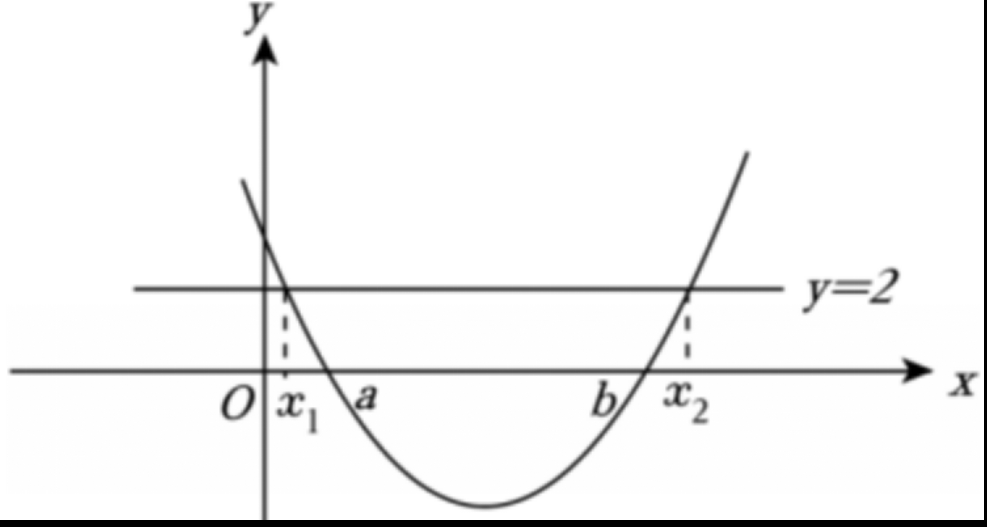
\includegraphics[width=0.42\textwidth]{figures/gao100_q16_parabola.png}
\end{center}
\step{所以数形结合得 $x_1<a<b<x_2$．故选 $B$.}
\solend
\fi

\end{enumerate}

\bigsec{三、解答题}

\begin{enumerate}
\setcounter{enumi}{16}

\item 已知集合 $A=\{x\mid3<x\leqslant6\}$，$B=\{x\mid m\leqslant x\leqslant2m+1\}$.

（1）若 $m=2$，求 $A\cap B$、$A\cup B$；

（2）若 $x\in B$ 是 $x\in A$ 的必要条件，求实数 $m$ 的取值范围.

\ansspace*[9]

\ifanswer
\solbegin
\stepm{（1）}{若 $m=2$，则 $B=\{x\mid2\leqslant x\leqslant5\}$，因为 $A=\{x\mid3<x\leqslant6\}$，}
\step{所以 $A\cap B=\{x\mid3<x\leqslant5\}$，$A\cup B=\{x\mid2\leqslant x\leqslant6\}$.}
\stepm{（2）}{因为 $x\in B$ 是 $x\in A$ 的必要条件，所以 $A\subseteq B$，}
\step{所以 $\begin{cases}m\leqslant3\\ 2m+1\geqslant6\end{cases}$，所以 $\dfrac52\leqslant m\leqslant3$，所以实数 $m$ 的取值范围为 $\left[\dfrac52,3\right]$.}
\solend
\fi

\item 求关于 $x$ 的不等式 $3ax^2-(3a+2)x+2<0\,(a\in R)$ 的解集.

\ansspace*[10]

\ifanswer
\solbegin
\step{当 $a=0$ 时，不等式化为 $-2x+2<0$，解得 $x>1$，}
\step{当 $a\neq0$ 时，方程 $3ax^2-(3a+2)x+2=0$ 的两根分别为 $1$，$\dfrac2{3a}$}
\step{当 $\dfrac2{3a}=1$，即 $a=\dfrac23$ 时，不等式化为 $(x-1)^2<0$，不等式无解，}
\step{当 $\dfrac2{3a}<1$，即 $a>\dfrac23$ 时，不等式解集为 $\left(\dfrac2{3a},1\right)$，}
\step{当 $0<a<\dfrac23$ 时，$\dfrac2{3a}>1$，不等式的解集为 $\left(1,\dfrac2{3a}\right)$，}
\step{当 $a<0$ 时，不等式的解集为 $\left(-\infty,\dfrac2{3a}\right)\cup(1,+\infty)$，}
\step{综上，当 $a=0$ 时，不等式的解集为 $(1,+\infty)$，}
\step{当 $a=\dfrac23$ 时，不等式的解集为 $\varnothing$，}
\step{当 $a>\dfrac23$ 时，不等式解集为 $\left(\dfrac2{3a},1\right)$，}
\step{当 $0<a<\dfrac23$ 时，不等式的解集为 $\left(1,\dfrac2{3a}\right)$，}
\step{当 $a<0$ 时，不等式的解集为 $\left(-\infty,\dfrac2{3a}\right)\cup(1,+\infty)$.}
\solend
\fi

\item 设对于任意实数 $x$，不等式 $\lvert x+1\rvert+\lvert x-1\rvert\geqslant m$ 恒成立.

（1）求 $m$ 的取值范围；

（2）当 $m$ 取最大值时，解关于 $x$ 的不等式 $\lvert x-3\rvert-2x\leqslant2m-2$.

\ansspace*[9]

\ifanswer
\solbegin
\stepm{（1）}{设函数 $f(x)=\lvert x+1\rvert+\lvert x-1\rvert$，则 $f(x)=\begin{cases}-2x,&x\leqslant-1\\ 2,&-1<x<1\\ 2x,&x\geqslant1\end{cases}$，}
\step{当 $x\leqslant-1$ 时，$f(x)$ 有最小值 2；}
\step{当 $-1<x<1$ 时，$f(x)=2$；}
\step{当 $x\geqslant1$ 时，$f(x)$ 有最小值 2；}
\step{因为对于任意实数 $x$，不等式 $\lvert x+1\rvert+\lvert x-1\rvert\geqslant m$ 恒成立，}
\step{所以 $m\leqslant2$，即 $m$ 的取值范围为 $(-\infty,2]$；}
\stepm{（2）}{由（1）得 $m$ 的最大值为 2，所以原不等式为 $\lvert x-3\rvert\leqslant2x+2$，}
\step{即 $-2x-2\leqslant x-3\leqslant2x+2$，解得 $x\geqslant\dfrac13$，}
\step{所以原不等式的解集为 $\left\{x\mid x\geqslant\dfrac13\right\}$.}
\solend
\fi

\item 某轮船公司的一艘轮船每小时花费的燃料费与轮船航行速度的平方成正比，比例系数为 $k$．轮船的最大速度为 18 海里/小时．当船速为 10 海里/小时，它的燃料费是每小时 120 元，其余航行运作费用（不论速度如何）总计是每小时 120 元．假定运行过程中轮船以速度 $v$ 匀速航行.

（1）求 $k$ 的值及每小时的最大总费用 $H$；

（2）求该轮船航行 100 海里的总费用 $W$（燃料费＋其余航行运作费用）的最小值.

\ansspace*[10]

\ifanswer
\solbegin
\stepm{（1）}{由题意，每小时燃料费为 $h(v)=kv^2$，$0<v\leqslant18$，}
\step{已知 $v=10$ 时，燃料费每小时 120 元，则 $k\cdot10^2=120$，得 $k=1.2$，}
\step{每小时总费用 $h(v)=kv^2+120=1.2v^2+120$，}
\step{$h(v)$ 是关于 $v$ 的增函数，$v$ 最大为 18，}
\step{所以 $H=h(18)=1.2\times18^2+120=508.8$ 元.}
\stepm{（2）}{航行时间 $t=\dfrac{100}v$ 小时，}
\step{$W(v)=h(v)\cdot t=(1.2v^2+120)\cdot\dfrac{100}v,0<v\leqslant18=120v+\dfrac{12000}v$，}
\step{利用均值不等式 $120v+\dfrac{12000}v\geqslant2\sqrt{120v\cdot\dfrac{12000}v}=2\times1200=2400$，}
\step{当且仅当 $120v=\dfrac{12000}v$，即 $v=10$ 时取等号，}
\step{$v=10\leqslant18$，在速度范围内，可取到等号，所以总费用最小值为 2400 元.}
\solend
\fi

\item 已知 $A$ 是 $R$ 的非空真子集，如果对任意 $x$、$y\in A$，都有 $x+y\in A$，$xy\in A$，则称 $A$ 是封闭集.

（1）判断集合 $B=\{0\}$，$C=\{-1,0,1\}$ 是否为封闭集，并说明理由；

（2）判断以下两个命题的真假，并说明理由；

命题 $p$：若非空集合 $A_1$、$A_2$ 是封闭集，则 $A_1\cup A_2$ 也是封闭集；

命题 $q$：非空集合 $A_1$、$A_2$ 是封闭集，则 $A_1\cap A_2\neq\varnothing$ 是 $A_1\cap A_2$ 是封闭集的充要条件；

（3）若非空集合 $A$ 是封闭集合，设全集为 $R$，求证：$A$ 的补集不是封闭集.

\ansspace*[13]

\ifanswer
\solbegin
\stepm{（1）}{$B=\{0\}$ 是封闭集，$C=\{-1,0,1\}$ 不是封闭集，理由如下：}
\step{对于集合 $B=\{0\}$，因为 $0+0=0\in B$，$0\times0=0\in B$，}
\step{所以 $B=\{0\}$ 是封闭集；}
\step{对于集合 $C=\{-1,0,1\}$，因为 $-1+(-1)=-2\notin C$，$1+1=2\notin C$，}
\step{所以集合 $C=\{-1,0,1\}$ 不是封闭集.}
\stepm{（2）}{命题 $p$ 是假命题，命题 $q$ 是真命题，理由如下：}
\step{对命题 $p$：令 $A_1=\{x\mid x=2k,k\in Z\}$，$A_2=\{x\mid x=3k,k\in Z\}$，}
\step{令 $x_1=2k_1$，$y_1=2k_2$，$k_1$、$k_2\in Z$，}
\step{则 $x_1+y_1=2(k_1+k_2)\in A_1$，$x_1y_1=2(2k_1k_2)\in A_1$，}
\step{因此集合 $A_1$ 是封闭集，同理集合 $A_2$ 也是封闭集，}
\step{取 $x_2=2$，$y_2=3$，则 $x_2$、$y_2\in(A_1\cup A_2)$，而 $x_2+y_2=5\notin(A_1\cup A_2)$，}
\step{因此集合 $A_1\cup A_2$ 不是封闭集，命题 $p$ 是假命题；}
\step{对于命题 $q$：若 $A_1\cap A_2\neq\varnothing$，不妨令 $a$、$b\in(A_1\cap A_2)$，}
\step{则有 $a$、$b\in A_1$，又集合 $A_1$ 是封闭集，则 $a+b\in A_1$，$ab\in A_1$，}
\step{同理 $a+b\in A_2$，$ab\in A_2$，因此 $a+b\in(A_1\cap A_2)$，$ab\in(A_1\cap A_2)$，}
\step{所以 $A_1\cap A_2$ 是封闭集；}
\step{反之，若 $A_1\cap A_2$ 是封闭集，则 $A_1\cap A_2$ 是非空集合，即 $A_1\cap A_2\neq\varnothing$，}
\step{所以 $A_1\cap A_2$ 是 $A_1\cap A_2$ 是封闭集的充要条件，命题 $q$ 是真命题.}
\stepm{（3）}{非空集合 $A$ 是封闭集合，当 $A=R$ 时，$\overline A=\varnothing$，因此 $\overline A$ 不是封闭集合；}
\step{当 $A\neq R$ 时，假设 $\overline A$ 是封闭集合，}
\step{设 $0\in A$，在 $\overline A$ 中任取一个 $x$，$x\neq0$，则 $-x\in A$，}
\step{否则 $-x\in\overline A$，此时 $x+(-x)=0\in\overline A$，与 $0\in A$ 矛盾，}
\step{因此 $(-x)^2\in A$，$x^2\in\overline A$，而 $(-x)^2=x^2$，与 $A\cap\overline A=\varnothing$ 矛盾，}
\step{则当 $0\in A$ 时，则 $\overline A$ 不是封闭集合，同理当 $0\in\overline A$ 时，$\overline A$ 不是封闭集合，}
\step{所以 $A$ 的补集不是封闭集.}
\solend
\fi

\end{enumerate}

\end{document}
"
%
% 原始材料：微信公众号“魔都数学加油站”文章，连载“27学年高一100”；
% 原文标题“27学年高一100——2026-2027年上海市南洋中学高一上10月月考”；
% 原文链接：https://mp.weixin.qq.com/s/uXLyt6VHraW4hSpDwnZDuQ。
% 正文为 10 张 PNG 页（`原图/高一100_南洋中学_10月月考/01..10.png`），
% 尺寸混排（第 2、4—9 页为 4762×6735，第 1、3、10 页为 2560×3620），按页序读取。
%
% 篇幅与题号：原卷自第 3 题起编号（第 1、2 题不在原文内）。填空题 3—12（10 题）、
% 选择题 13—16（4 题）、解答题 17—21（5 题），共 19 题。
%
% 讲评版：全部 19 题均印【解析】，其中第 13—16 题的答案在解析末句
% “故选 $C$／$B$／$D$／$B$”（题干括号内未印答案）。第 16 题解析带一幅
% 抛物线与 $y=2$ 的示意图，自原图裁切、去粉色水印后转灰度，三版都出。
%
% 副标题：原卷未印副标题。本稿按内容标作“集合与常用逻辑用语、不等式”。
%
% 原卷笔误/存疑（均照录未改，正文对应处另有 % 注）：无。
%
% 与原卷的排版差异：
%   ① 原卷每题下直接印【解析】，本稿按全稿惯例将答案与解析置于答案版；
%   ② 原卷未印副标题，本稿补出；填空横线统一排 \blankline[4.4em]；
%   ③ 原卷数集记号排斜体 $R$、$Z$、$\mathit N$，本稿按全稿惯例改用 $\R$、$\Z$、$\N$；
%   ④ 解答题按惯例加 \ansspace；选择题括号排 \mbox{（\quad）}；
%   ⑤ 第 16 题的示意图原卷排在解析行右侧，本稿改排为解析后的居中图。
%
% 行数核对：逐题数 \step/\stepm 条数，合计 117 条（Q3：2；Q4：5；Q5：7；Q6：3；Q7：3；
% Q8：4；Q9：2；Q10：4；Q11：6；Q12：3；Q13：7；Q14：3；Q15：5；Q16：3；Q17：5；
% Q18：11；Q19：9；Q20：10；Q21：25）。全卷 19 题均印【解析】。
% 原卷解析的换行按语意合并，未逐行强拆。
%
\documentclass[a4paper,11pt]{article}
\usepackage{common}
\begin{document}

\examtitlest[7]{2026--2027 年南洋中学高一上 10 月月考}{集合与常用逻辑用语、不等式}

\bigsec{一、填空题}

\begin{enumerate}
\setcounter{enumi}{2}

\item 不等式 $\dfrac{x-6}{x+1}\geqslant0$ 的解集为\blankline[4.4em].

\ifanswer
\solbegin
\step{不等式 $\dfrac{x-6}{x+1}\geqslant0$ 等价于 $\begin{cases}(x-6)(x+1)\geqslant0\\ x+1\neq0\end{cases}$，即 $x<-1$ 或 $x\geqslant6$，}
\step{故解集为 $(-\infty,-1)\cup[6,+\infty)$.}
\solend
\fi

\item 已知关于 $x$ 的不等式 $ax^2+bx+c>0$ 的解集是 $(1,3)$，则关于 $x$ 的不等式 $ax^2-bx+c\leqslant0$ 的解集为\blankline[4.4em].

\ifanswer
\solbegin
\step{由已知得 $a<0$，且 $1$，$3$ 是方程 $ax^2+bx+c=0$ 的根，}
\step{所以 $\begin{cases}1+3=-\dfrac ba\\[2pt] 1\times3=\dfrac ca\end{cases}$，所以 $\begin{cases}b=-4a\\ c=3a\end{cases}$，}
\step{所以 $ax^2-bx+c\leqslant0$ 可变形为 $ax^2+4ax+3a\leqslant0$，}
\step{因为 $a<0$，所以 $x^2+4x+3\geqslant0$，解得 $x\leqslant-3$ 或 $x\geqslant-1$，}
\step{所以不等式的解集为 $(-\infty,-3]\cup[-1,+\infty)$.}
\solend
\fi

\item 不等式 $\lvert x+2\rvert+\lvert 2x-1\rvert\geqslant3$ 的解集为\blankline[4.4em].

\ifanswer
\solbegin
\step{当 $x\leqslant-2$ 时，$x+2\leqslant0$，$2x-1<0$，}
\step{所以 $\lvert x+2\rvert+\lvert 2x-1\rvert=-x-2-2x+1\geqslant3$，解得 $x\leqslant-\dfrac43$；}
\step{当 $-2<x<\dfrac12$ 时，$x+2>0$，$2x-1<0$，}
\step{所以 $\lvert x+2\rvert+\lvert 2x-1\rvert=x+2-2x+1\geqslant3$，解得 $x\leqslant0$；}
\step{当 $x\geqslant\dfrac12$ 时，$x+2>0$，$2x-1\geqslant0$，}
\step{所以 $\lvert x+2\rvert+\lvert 2x-1\rvert=x+2+2x-1\geqslant3$，解得 $x\geqslant\dfrac23$；}
\step{所以原不等式的解集为 $\left\{x\mid x\leqslant0\right.$ 或 $\left.x\geqslant\dfrac23\right\}$.}
\solend
\fi

\item 若正数 $x$、$y$ 满足 $x+2y=2$，则 $\dfrac1x+\dfrac2y$ 的最小值是\blankline[4.4em].

\ifanswer
\solbegin
\step{因为 $x>0$，$y>0$，且 $x+2y=2$，}
\step{所以 $\dfrac1x+\dfrac2y=\dfrac12\left(\dfrac1x+\dfrac2y\right)(x+2y)=\dfrac12\left(5+\dfrac{2y}x+\dfrac{2x}y\right)\geqslant\dfrac12\left(5+2\sqrt{\dfrac{2y}x\cdot\dfrac{2x}y}\right)=\dfrac92$.}
\step{当且仅当 $\begin{cases}x+2y=2\\ \dfrac{2y}x=\dfrac{2x}y\end{cases}$，即 $x=y=\dfrac23$ 时取等号，故最小值为 $\dfrac92$.}
\solend
\fi

\item 已知 $\alpha:x\leqslant2$ 或 $x>3$，$\beta:x\leqslant m+5$ 或 $x>-m$，若 $\alpha$ 是 $\beta$ 的必要非充分条件，则实数 $m$ 的取值范围是\blankline[4.4em].

\ifanswer
\solbegin
\step{设 $A=\{x\mid x\leqslant2$ 或 $x>3\}$，$B=\{x\mid x\leqslant m+5$ 或 $x>-m\}$，则 $B\subset A$，}
\step{则 $m+5\leqslant2$ 且 $-m\geqslant3$（等号不能同时取得），则 $m<-3$，}
\step{则实数 $m$ 的取值范围是 $(-\infty,-3)$.}
\solend
\fi

\item 已知集合 $A=\{x\mid-1\leqslant x\leqslant3\}$，$B=\{x\mid ax+1>0\}$ 满足 $A\subseteq B$，则实数 $a$ 的取值范围为\blankline[4.4em].

\ifanswer
\solbegin
\step{当 $a=0$ 时，$B=R$，显然符合题意，}
\step{当 $a>0$ 时，$B=\left\{x\mid x>-\dfrac1a\right\}$，则 $-\dfrac1a<-1$，解得 $a<1$，所以 $0<a<1$，}
\step{当 $a<0$ 时，$B=\left\{x\mid x<-\dfrac1a\right\}$，则 $-\dfrac1a>3$，解得 $a>-\dfrac13$，所以 $-\dfrac13<a<0$，}
\step{综上所述，实数 $a$ 的取值范围为 $\left(-\dfrac13,1\right)$.}
\solend
\fi

\item 设集合 $A=\{x\mid3x-1<m\}$，若 $1\in A$ 且 $2\notin A$，则实数 $m$ 的取值范围是\blankline[4.4em].

\ifanswer
\solbegin
\step{因为集合 $A=\{x\mid3x-1<m\}$，若 $1\in A$ 且 $2\notin A$，}
\step{则 $3\times1-1<m$ 且 $3\times2-1\geqslant m$，解得 $2<m\leqslant5$.}
\solend
\fi

\item 若 $M=\left\{x\mid x=m+\dfrac16,m\in Z\right\},N=\left\{x\mid x=\dfrac n2-\dfrac13,n\in Z\right\}$，\newline $P=\left\{x\mid x=\dfrac p2+\dfrac16,p\in Z\right\}$，则 $M$、$N$、$P$ 的关系为\blankline[4.4em].

\ifanswer
\solbegin
\step{$M=\left\{x\mid x=m+\dfrac16=\dfrac{6m+1}6=\dfrac{3\cdot2m+1}6,m\in Z\right\}$，}
\step{$N=\left\{x\mid x=\dfrac n2-\dfrac13=\dfrac{3(n-1)+1}6,n\in Z\right\}=\left\{x\mid x=\dfrac{3k+1}6,k\in Z\right\}$，}
\step{$P=\left\{x\mid x=\dfrac p2+\dfrac16=\dfrac{3p+1}6,p\in Z\right\}$，}
\step{故 $M\subset N=P$.}
\solend
\fi

\item 已知命题 $p:x<-2$ 或 $x>3$，命题 $q:x<3m+1$ 或 $x>m+2$，若 $p$ 是 $q$ 的充分非必要条件，则实数 $m$ 的取值范围是\blankline[4.4em].

\ifanswer
\solbegin
\step{设 $A=\{x\mid x<-2$ 或 $x>3\}$，$B=\{x\mid x<3m+1$ 或 $x>m+2\}$，}
\step{若 $p$ 是 $q$ 的充分非必要条件，则 $A\subset B$，}
\step{当 $3m+1\geqslant m+2$，即 $m\geqslant\dfrac12$ 时，显然有 $A\subset B$，}
\step{当 $3m+1<m+2$，即 $m<\dfrac12$ 时，}
\step{由 $A\subset B$，则 $\begin{cases}m+2\leqslant3\\ 3m+1\geqslant-2\end{cases}$（等号不同时成立），即 $-1\leqslant m<\dfrac12$.}
\step{综上，实数 $m$ 的取值范围是 $[-1,+\infty)$.}
\solend
\fi

\item 对于一个有限集 $A$，一般都可以找到两个非空数集 $A_1$ 和 $A_2$，满足 $A_1\cap A_2=\varnothing$，且 $A_1\cup A_2=A$，记集合 $\{A_1,A_2\}$ 为 $A$ 的一个“划分集”．若 $A$ 中有 $n(n\geqslant2,n\in\N)$ 个元素，则不同的“划分集”共有\blankline[4.4em]个(用含 $n$ 的表达式填空).

\ifanswer
\solbegin
\step{集合中的每个元素都有属于 $A_1$ 或属于 $A_2$ 两种情况，故共有 $2^n$ 种情况，}
\step{排除全都属于 $A_1$ 或 $A_2$ 的两种情况，考虑对称情况，}
\step{故不同的“划分集”共有 $\dfrac12(2^n-2)=2^{n-1}-1$ 个.}
\solend
\fi

\end{enumerate}

\bigsec{二、选择题}

\begin{enumerate}
\setcounter{enumi}{12}

\item 下列命题中正确的\mbox{（\quad）}

\keepwithprev
A. $\varnothing$ 与 $\{0\}$ 表示同一个集合

B. 方程 $\{x\mid(x-2)^2(x-3)=0\}$ 的所有解的集合可表示为 $\{2,2,3\}$

C. 由 3，4，5 组成的集合可表示为 $\{3,4,5\}$ 或 $\{4,5,3\}$

D. 很小的实数可以构成集合.

\ifanswer
\solbegin
\step{对于 $A$，$\{0\}$ 中有一个元素 0，$\varnothing$ 中无任何元素，故 $\varnothing$ 与 $\{0\}$ 不是同一个集合，}
\step{故 $A$ 错误；}
\step{对于 $B$，$\{2,2,3\}$ 不满足集合元素的互异性，故 $B$ 错误；}
\step{对于 $C$，由集合的无序性，得由 3，4，5 组成的集合可表示为 $\{3,4,5\}$ 或 $\{4,5,3\}$，}
\step{故 $C$ 正确；}
\step{对于 $D$，由集合的确定性，很小的实数不能构成集合，故 $D$ 错误.}
\step{故选 $C$.}
\solend
\fi

\item 已知 $a\in R$，则“$\dfrac1a<1$”是“$a>1$”的\mbox{（\quad）}条件.

\keepwithprev
A. 充分非必要\qquad B. 必要非充分

C. 充要\qquad D. 既非充分又非必要

\ifanswer
\solbegin
\step{解 $\dfrac1a<1$，得 $a<0$ 或 $a>1$，}
\step{由 $a<0$ 或 $a>1$ 得不出 $a>1$，由 $a>1$ 得出 $a<0$ 或 $a>1$，}
\step{所以“$\dfrac1a<1$”是“$a>1$”的必要不充分条件．故选 $B$.}
\solend
\fi

\item 若命题“存在 $x_0\in R$ 使得 $ax_0^2+2ax_0+1\leqslant0$”是假命题，则实数 $a$ 的取值范围为\mbox{（\quad）}

\keepwithprev
A. $a<0$ 或 $a\geqslant1$\qquad B. $a\leqslant0$ 或 $a\geqslant1$\qquad C. $0<a<1$\qquad D. $0\leqslant a<1$

\ifanswer
\solbegin
\step{命题“存在 $x_0\in R$ 使得 $ax_0^2+2ax_0+1\leqslant0$”是假命题，}
\step{则 $\forall x\in R$，$ax^2+2ax+1>0$ 恒成立，}
\step{当 $a=0$ 时，满足题意，}
\step{当 $a\neq0$ 时，$\begin{cases}a>0\\ \Delta=4a^2-4a<0\end{cases}$，解得 $0<a<1$，}
\step{综上所述，实数 $a$ 的取值范围为 $\{a\mid0\leqslant a<1\}$．故选 $D$.}
\solend
\fi

\item 已知实数 $a<b$，关于 $x$ 的不等式 $x^2-(a+b)x+ab-2<0$ 的解集为 $(x_1,x_2)$，则实数 $a$、$b$、$x_1$、$x_2$ 从小到大的排列是\mbox{（\quad）}

\keepwithprev
A. $a<x_1<x_2<b$\qquad B. $x_1<a<b<x_2$\qquad C. $a<x_1<b<x_2$\qquad D. $x_1<a<x_2<b$

\ifanswer
\solbegin
\step{因为实数 $a<b$，不等式 $x^2-(a+b)x+ab-2<0$ 可化为 $(x-a)(x-b)<2$，}
\step{又其解集为 $(x_1,x_2)$，所以作出 $y=(x-a)(x-b)$ 与 $y=2$ 的图象如下：}
\begin{center}
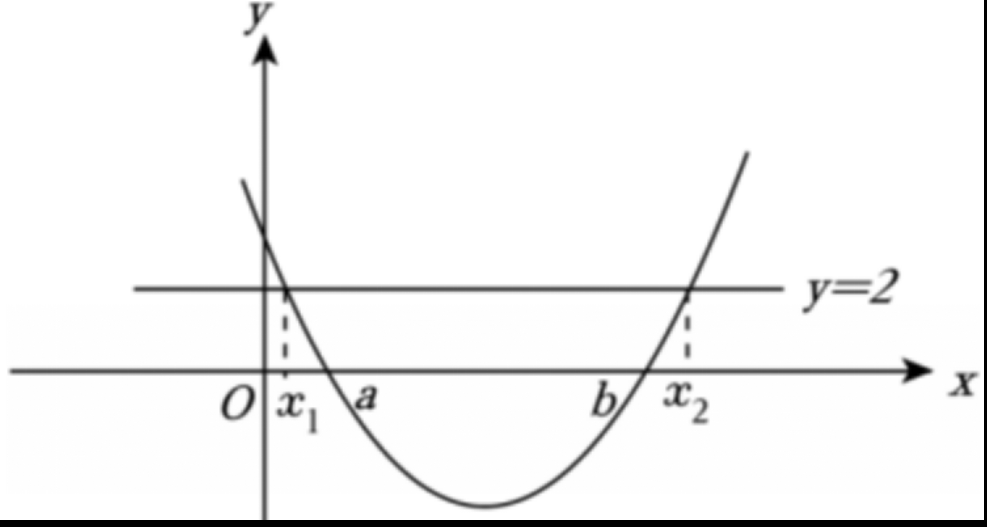
\includegraphics[width=0.42\textwidth]{figures/gao100_q16_parabola.png}
\end{center}
\step{所以数形结合得 $x_1<a<b<x_2$．故选 $B$.}
\solend
\fi

\end{enumerate}

\bigsec{三、解答题}

\begin{enumerate}
\setcounter{enumi}{16}

\item 已知集合 $A=\{x\mid3<x\leqslant6\}$，$B=\{x\mid m\leqslant x\leqslant2m+1\}$.

（1）若 $m=2$，求 $A\cap B$、$A\cup B$；

（2）若 $x\in B$ 是 $x\in A$ 的必要条件，求实数 $m$ 的取值范围.

\ansspace*[9]

\ifanswer
\solbegin
\stepm{（1）}{若 $m=2$，则 $B=\{x\mid2\leqslant x\leqslant5\}$，因为 $A=\{x\mid3<x\leqslant6\}$，}
\step{所以 $A\cap B=\{x\mid3<x\leqslant5\}$，$A\cup B=\{x\mid2\leqslant x\leqslant6\}$.}
\stepm{（2）}{因为 $x\in B$ 是 $x\in A$ 的必要条件，所以 $A\subseteq B$，}
\step{所以 $\begin{cases}m\leqslant3\\ 2m+1\geqslant6\end{cases}$，所以 $\dfrac52\leqslant m\leqslant3$，所以实数 $m$ 的取值范围为 $\left[\dfrac52,3\right]$.}
\solend
\fi

\item 求关于 $x$ 的不等式 $3ax^2-(3a+2)x+2<0\,(a\in R)$ 的解集.

\ansspace*[10]

\ifanswer
\solbegin
\step{当 $a=0$ 时，不等式化为 $-2x+2<0$，解得 $x>1$，}
\step{当 $a\neq0$ 时，方程 $3ax^2-(3a+2)x+2=0$ 的两根分别为 $1$，$\dfrac2{3a}$}
\step{当 $\dfrac2{3a}=1$，即 $a=\dfrac23$ 时，不等式化为 $(x-1)^2<0$，不等式无解，}
\step{当 $\dfrac2{3a}<1$，即 $a>\dfrac23$ 时，不等式解集为 $\left(\dfrac2{3a},1\right)$，}
\step{当 $0<a<\dfrac23$ 时，$\dfrac2{3a}>1$，不等式的解集为 $\left(1,\dfrac2{3a}\right)$，}
\step{当 $a<0$ 时，不等式的解集为 $\left(-\infty,\dfrac2{3a}\right)\cup(1,+\infty)$，}
\step{综上，当 $a=0$ 时，不等式的解集为 $(1,+\infty)$，}
\step{当 $a=\dfrac23$ 时，不等式的解集为 $\varnothing$，}
\step{当 $a>\dfrac23$ 时，不等式解集为 $\left(\dfrac2{3a},1\right)$，}
\step{当 $0<a<\dfrac23$ 时，不等式的解集为 $\left(1,\dfrac2{3a}\right)$，}
\step{当 $a<0$ 时，不等式的解集为 $\left(-\infty,\dfrac2{3a}\right)\cup(1,+\infty)$.}
\solend
\fi

\item 设对于任意实数 $x$，不等式 $\lvert x+1\rvert+\lvert x-1\rvert\geqslant m$ 恒成立.

（1）求 $m$ 的取值范围；

（2）当 $m$ 取最大值时，解关于 $x$ 的不等式 $\lvert x-3\rvert-2x\leqslant2m-2$.

\ansspace*[9]

\ifanswer
\solbegin
\stepm{（1）}{设函数 $f(x)=\lvert x+1\rvert+\lvert x-1\rvert$，则 $f(x)=\begin{cases}-2x,&x\leqslant-1\\ 2,&-1<x<1\\ 2x,&x\geqslant1\end{cases}$，}
\step{当 $x\leqslant-1$ 时，$f(x)$ 有最小值 2；}
\step{当 $-1<x<1$ 时，$f(x)=2$；}
\step{当 $x\geqslant1$ 时，$f(x)$ 有最小值 2；}
\step{因为对于任意实数 $x$，不等式 $\lvert x+1\rvert+\lvert x-1\rvert\geqslant m$ 恒成立，}
\step{所以 $m\leqslant2$，即 $m$ 的取值范围为 $(-\infty,2]$；}
\stepm{（2）}{由（1）得 $m$ 的最大值为 2，所以原不等式为 $\lvert x-3\rvert\leqslant2x+2$，}
\step{即 $-2x-2\leqslant x-3\leqslant2x+2$，解得 $x\geqslant\dfrac13$，}
\step{所以原不等式的解集为 $\left\{x\mid x\geqslant\dfrac13\right\}$.}
\solend
\fi

\item 某轮船公司的一艘轮船每小时花费的燃料费与轮船航行速度的平方成正比，比例系数为 $k$．轮船的最大速度为 18 海里/小时．当船速为 10 海里/小时，它的燃料费是每小时 120 元，其余航行运作费用（不论速度如何）总计是每小时 120 元．假定运行过程中轮船以速度 $v$ 匀速航行.

（1）求 $k$ 的值及每小时的最大总费用 $H$；

（2）求该轮船航行 100 海里的总费用 $W$（燃料费＋其余航行运作费用）的最小值.

\ansspace*[10]

\ifanswer
\solbegin
\stepm{（1）}{由题意，每小时燃料费为 $h(v)=kv^2$，$0<v\leqslant18$，}
\step{已知 $v=10$ 时，燃料费每小时 120 元，则 $k\cdot10^2=120$，得 $k=1.2$，}
\step{每小时总费用 $h(v)=kv^2+120=1.2v^2+120$，}
\step{$h(v)$ 是关于 $v$ 的增函数，$v$ 最大为 18，}
\step{所以 $H=h(18)=1.2\times18^2+120=508.8$ 元.}
\stepm{（2）}{航行时间 $t=\dfrac{100}v$ 小时，}
\step{$W(v)=h(v)\cdot t=(1.2v^2+120)\cdot\dfrac{100}v,0<v\leqslant18=120v+\dfrac{12000}v$，}
\step{利用均值不等式 $120v+\dfrac{12000}v\geqslant2\sqrt{120v\cdot\dfrac{12000}v}=2\times1200=2400$，}
\step{当且仅当 $120v=\dfrac{12000}v$，即 $v=10$ 时取等号，}
\step{$v=10\leqslant18$，在速度范围内，可取到等号，所以总费用最小值为 2400 元.}
\solend
\fi

\item 已知 $A$ 是 $R$ 的非空真子集，如果对任意 $x$、$y\in A$，都有 $x+y\in A$，$xy\in A$，则称 $A$ 是封闭集.

（1）判断集合 $B=\{0\}$，$C=\{-1,0,1\}$ 是否为封闭集，并说明理由；

（2）判断以下两个命题的真假，并说明理由；

命题 $p$：若非空集合 $A_1$、$A_2$ 是封闭集，则 $A_1\cup A_2$ 也是封闭集；

命题 $q$：非空集合 $A_1$、$A_2$ 是封闭集，则 $A_1\cap A_2\neq\varnothing$ 是 $A_1\cap A_2$ 是封闭集的充要条件；

（3）若非空集合 $A$ 是封闭集合，设全集为 $R$，求证：$A$ 的补集不是封闭集.

\ansspace*[13]

\ifanswer
\solbegin
\stepm{（1）}{$B=\{0\}$ 是封闭集，$C=\{-1,0,1\}$ 不是封闭集，理由如下：}
\step{对于集合 $B=\{0\}$，因为 $0+0=0\in B$，$0\times0=0\in B$，}
\step{所以 $B=\{0\}$ 是封闭集；}
\step{对于集合 $C=\{-1,0,1\}$，因为 $-1+(-1)=-2\notin C$，$1+1=2\notin C$，}
\step{所以集合 $C=\{-1,0,1\}$ 不是封闭集.}
\stepm{（2）}{命题 $p$ 是假命题，命题 $q$ 是真命题，理由如下：}
\step{对命题 $p$：令 $A_1=\{x\mid x=2k,k\in Z\}$，$A_2=\{x\mid x=3k,k\in Z\}$，}
\step{令 $x_1=2k_1$，$y_1=2k_2$，$k_1$、$k_2\in Z$，}
\step{则 $x_1+y_1=2(k_1+k_2)\in A_1$，$x_1y_1=2(2k_1k_2)\in A_1$，}
\step{因此集合 $A_1$ 是封闭集，同理集合 $A_2$ 也是封闭集，}
\step{取 $x_2=2$，$y_2=3$，则 $x_2$、$y_2\in(A_1\cup A_2)$，而 $x_2+y_2=5\notin(A_1\cup A_2)$，}
\step{因此集合 $A_1\cup A_2$ 不是封闭集，命题 $p$ 是假命题；}
\step{对于命题 $q$：若 $A_1\cap A_2\neq\varnothing$，不妨令 $a$、$b\in(A_1\cap A_2)$，}
\step{则有 $a$、$b\in A_1$，又集合 $A_1$ 是封闭集，则 $a+b\in A_1$，$ab\in A_1$，}
\step{同理 $a+b\in A_2$，$ab\in A_2$，因此 $a+b\in(A_1\cap A_2)$，$ab\in(A_1\cap A_2)$，}
\step{所以 $A_1\cap A_2$ 是封闭集；}
\step{反之，若 $A_1\cap A_2$ 是封闭集，则 $A_1\cap A_2$ 是非空集合，即 $A_1\cap A_2\neq\varnothing$，}
\step{所以 $A_1\cap A_2$ 是 $A_1\cap A_2$ 是封闭集的充要条件，命题 $q$ 是真命题.}
\stepm{（3）}{非空集合 $A$ 是封闭集合，当 $A=R$ 时，$\overline A=\varnothing$，因此 $\overline A$ 不是封闭集合；}
\step{当 $A\neq R$ 时，假设 $\overline A$ 是封闭集合，}
\step{设 $0\in A$，在 $\overline A$ 中任取一个 $x$，$x\neq0$，则 $-x\in A$，}
\step{否则 $-x\in\overline A$，此时 $x+(-x)=0\in\overline A$，与 $0\in A$ 矛盾，}
\step{因此 $(-x)^2\in A$，$x^2\in\overline A$，而 $(-x)^2=x^2$，与 $A\cap\overline A=\varnothing$ 矛盾，}
\step{则当 $0\in A$ 时，则 $\overline A$ 不是封闭集合，同理当 $0\in\overline A$ 时，$\overline A$ 不是封闭集合，}
\step{所以 $A$ 的补集不是封闭集.}
\solend
\fi

\end{enumerate}

\end{document}
"
% 紧凑版：xelatex "\def\iscompact{1}% 高一100_南洋中学_10月月考.tex
%   —— 高一上数学“2026-2027 年南洋中学高一上 10 月月考”（讲评版）
% 试卷版：xelatex 高一100_南洋中学_10月月考.tex
% 答案版：xelatex "\def\isanswer{1}% 高一100_南洋中学_10月月考.tex
%   —— 高一上数学“2026-2027 年南洋中学高一上 10 月月考”（讲评版）
% 试卷版：xelatex 高一100_南洋中学_10月月考.tex
% 答案版：xelatex "\def\isanswer{1}\input{高一100_南洋中学_10月月考.tex}"
% 紧凑版：xelatex "\def\iscompact{1}\input{高一100_南洋中学_10月月考.tex}"
%
% 原始材料：微信公众号“魔都数学加油站”文章，连载“27学年高一100”；
% 原文标题“27学年高一100——2026-2027年上海市南洋中学高一上10月月考”；
% 原文链接：https://mp.weixin.qq.com/s/uXLyt6VHraW4hSpDwnZDuQ。
% 正文为 10 张 PNG 页（`原图/高一100_南洋中学_10月月考/01..10.png`），
% 尺寸混排（第 2、4—9 页为 4762×6735，第 1、3、10 页为 2560×3620），按页序读取。
%
% 篇幅与题号：原卷自第 3 题起编号（第 1、2 题不在原文内）。填空题 3—12（10 题）、
% 选择题 13—16（4 题）、解答题 17—21（5 题），共 19 题。
%
% 讲评版：全部 19 题均印【解析】，其中第 13—16 题的答案在解析末句
% “故选 $C$／$B$／$D$／$B$”（题干括号内未印答案）。第 16 题解析带一幅
% 抛物线与 $y=2$ 的示意图，自原图裁切、去粉色水印后转灰度，三版都出。
%
% 副标题：原卷未印副标题。本稿按内容标作“集合与常用逻辑用语、不等式”。
%
% 原卷笔误/存疑（均照录未改，正文对应处另有 % 注）：无。
%
% 与原卷的排版差异：
%   ① 原卷每题下直接印【解析】，本稿按全稿惯例将答案与解析置于答案版；
%   ② 原卷未印副标题，本稿补出；填空横线统一排 \blankline[4.4em]；
%   ③ 原卷数集记号排斜体 $R$、$Z$、$\mathit N$，本稿按全稿惯例改用 $\R$、$\Z$、$\N$；
%   ④ 解答题按惯例加 \ansspace；选择题括号排 \mbox{（\quad）}；
%   ⑤ 第 16 题的示意图原卷排在解析行右侧，本稿改排为解析后的居中图。
%
% 行数核对：逐题数 \step/\stepm 条数，合计 117 条（Q3：2；Q4：5；Q5：7；Q6：3；Q7：3；
% Q8：4；Q9：2；Q10：4；Q11：6；Q12：3；Q13：7；Q14：3；Q15：5；Q16：3；Q17：5；
% Q18：11；Q19：9；Q20：10；Q21：25）。全卷 19 题均印【解析】。
% 原卷解析的换行按语意合并，未逐行强拆。
%
\documentclass[a4paper,11pt]{article}
\usepackage{common}
\begin{document}

\examtitlest[7]{2026--2027 年南洋中学高一上 10 月月考}{集合与常用逻辑用语、不等式}

\bigsec{一、填空题}

\begin{enumerate}
\setcounter{enumi}{2}

\item 不等式 $\dfrac{x-6}{x+1}\geqslant0$ 的解集为\blankline[4.4em].

\ifanswer
\solbegin
\step{不等式 $\dfrac{x-6}{x+1}\geqslant0$ 等价于 $\begin{cases}(x-6)(x+1)\geqslant0\\ x+1\neq0\end{cases}$，即 $x<-1$ 或 $x\geqslant6$，}
\step{故解集为 $(-\infty,-1)\cup[6,+\infty)$.}
\solend
\fi

\item 已知关于 $x$ 的不等式 $ax^2+bx+c>0$ 的解集是 $(1,3)$，则关于 $x$ 的不等式 $ax^2-bx+c\leqslant0$ 的解集为\blankline[4.4em].

\ifanswer
\solbegin
\step{由已知得 $a<0$，且 $1$，$3$ 是方程 $ax^2+bx+c=0$ 的根，}
\step{所以 $\begin{cases}1+3=-\dfrac ba\\[2pt] 1\times3=\dfrac ca\end{cases}$，所以 $\begin{cases}b=-4a\\ c=3a\end{cases}$，}
\step{所以 $ax^2-bx+c\leqslant0$ 可变形为 $ax^2+4ax+3a\leqslant0$，}
\step{因为 $a<0$，所以 $x^2+4x+3\geqslant0$，解得 $x\leqslant-3$ 或 $x\geqslant-1$，}
\step{所以不等式的解集为 $(-\infty,-3]\cup[-1,+\infty)$.}
\solend
\fi

\item 不等式 $\lvert x+2\rvert+\lvert 2x-1\rvert\geqslant3$ 的解集为\blankline[4.4em].

\ifanswer
\solbegin
\step{当 $x\leqslant-2$ 时，$x+2\leqslant0$，$2x-1<0$，}
\step{所以 $\lvert x+2\rvert+\lvert 2x-1\rvert=-x-2-2x+1\geqslant3$，解得 $x\leqslant-\dfrac43$；}
\step{当 $-2<x<\dfrac12$ 时，$x+2>0$，$2x-1<0$，}
\step{所以 $\lvert x+2\rvert+\lvert 2x-1\rvert=x+2-2x+1\geqslant3$，解得 $x\leqslant0$；}
\step{当 $x\geqslant\dfrac12$ 时，$x+2>0$，$2x-1\geqslant0$，}
\step{所以 $\lvert x+2\rvert+\lvert 2x-1\rvert=x+2+2x-1\geqslant3$，解得 $x\geqslant\dfrac23$；}
\step{所以原不等式的解集为 $\left\{x\mid x\leqslant0\right.$ 或 $\left.x\geqslant\dfrac23\right\}$.}
\solend
\fi

\item 若正数 $x$、$y$ 满足 $x+2y=2$，则 $\dfrac1x+\dfrac2y$ 的最小值是\blankline[4.4em].

\ifanswer
\solbegin
\step{因为 $x>0$，$y>0$，且 $x+2y=2$，}
\step{所以 $\dfrac1x+\dfrac2y=\dfrac12\left(\dfrac1x+\dfrac2y\right)(x+2y)=\dfrac12\left(5+\dfrac{2y}x+\dfrac{2x}y\right)\geqslant\dfrac12\left(5+2\sqrt{\dfrac{2y}x\cdot\dfrac{2x}y}\right)=\dfrac92$.}
\step{当且仅当 $\begin{cases}x+2y=2\\ \dfrac{2y}x=\dfrac{2x}y\end{cases}$，即 $x=y=\dfrac23$ 时取等号，故最小值为 $\dfrac92$.}
\solend
\fi

\item 已知 $\alpha:x\leqslant2$ 或 $x>3$，$\beta:x\leqslant m+5$ 或 $x>-m$，若 $\alpha$ 是 $\beta$ 的必要非充分条件，则实数 $m$ 的取值范围是\blankline[4.4em].

\ifanswer
\solbegin
\step{设 $A=\{x\mid x\leqslant2$ 或 $x>3\}$，$B=\{x\mid x\leqslant m+5$ 或 $x>-m\}$，则 $B\subset A$，}
\step{则 $m+5\leqslant2$ 且 $-m\geqslant3$（等号不能同时取得），则 $m<-3$，}
\step{则实数 $m$ 的取值范围是 $(-\infty,-3)$.}
\solend
\fi

\item 已知集合 $A=\{x\mid-1\leqslant x\leqslant3\}$，$B=\{x\mid ax+1>0\}$ 满足 $A\subseteq B$，则实数 $a$ 的取值范围为\blankline[4.4em].

\ifanswer
\solbegin
\step{当 $a=0$ 时，$B=R$，显然符合题意，}
\step{当 $a>0$ 时，$B=\left\{x\mid x>-\dfrac1a\right\}$，则 $-\dfrac1a<-1$，解得 $a<1$，所以 $0<a<1$，}
\step{当 $a<0$ 时，$B=\left\{x\mid x<-\dfrac1a\right\}$，则 $-\dfrac1a>3$，解得 $a>-\dfrac13$，所以 $-\dfrac13<a<0$，}
\step{综上所述，实数 $a$ 的取值范围为 $\left(-\dfrac13,1\right)$.}
\solend
\fi

\item 设集合 $A=\{x\mid3x-1<m\}$，若 $1\in A$ 且 $2\notin A$，则实数 $m$ 的取值范围是\blankline[4.4em].

\ifanswer
\solbegin
\step{因为集合 $A=\{x\mid3x-1<m\}$，若 $1\in A$ 且 $2\notin A$，}
\step{则 $3\times1-1<m$ 且 $3\times2-1\geqslant m$，解得 $2<m\leqslant5$.}
\solend
\fi

\item 若 $M=\left\{x\mid x=m+\dfrac16,m\in Z\right\},N=\left\{x\mid x=\dfrac n2-\dfrac13,n\in Z\right\}$，\newline $P=\left\{x\mid x=\dfrac p2+\dfrac16,p\in Z\right\}$，则 $M$、$N$、$P$ 的关系为\blankline[4.4em].

\ifanswer
\solbegin
\step{$M=\left\{x\mid x=m+\dfrac16=\dfrac{6m+1}6=\dfrac{3\cdot2m+1}6,m\in Z\right\}$，}
\step{$N=\left\{x\mid x=\dfrac n2-\dfrac13=\dfrac{3(n-1)+1}6,n\in Z\right\}=\left\{x\mid x=\dfrac{3k+1}6,k\in Z\right\}$，}
\step{$P=\left\{x\mid x=\dfrac p2+\dfrac16=\dfrac{3p+1}6,p\in Z\right\}$，}
\step{故 $M\subset N=P$.}
\solend
\fi

\item 已知命题 $p:x<-2$ 或 $x>3$，命题 $q:x<3m+1$ 或 $x>m+2$，若 $p$ 是 $q$ 的充分非必要条件，则实数 $m$ 的取值范围是\blankline[4.4em].

\ifanswer
\solbegin
\step{设 $A=\{x\mid x<-2$ 或 $x>3\}$，$B=\{x\mid x<3m+1$ 或 $x>m+2\}$，}
\step{若 $p$ 是 $q$ 的充分非必要条件，则 $A\subset B$，}
\step{当 $3m+1\geqslant m+2$，即 $m\geqslant\dfrac12$ 时，显然有 $A\subset B$，}
\step{当 $3m+1<m+2$，即 $m<\dfrac12$ 时，}
\step{由 $A\subset B$，则 $\begin{cases}m+2\leqslant3\\ 3m+1\geqslant-2\end{cases}$（等号不同时成立），即 $-1\leqslant m<\dfrac12$.}
\step{综上，实数 $m$ 的取值范围是 $[-1,+\infty)$.}
\solend
\fi

\item 对于一个有限集 $A$，一般都可以找到两个非空数集 $A_1$ 和 $A_2$，满足 $A_1\cap A_2=\varnothing$，且 $A_1\cup A_2=A$，记集合 $\{A_1,A_2\}$ 为 $A$ 的一个“划分集”．若 $A$ 中有 $n(n\geqslant2,n\in\N)$ 个元素，则不同的“划分集”共有\blankline[4.4em]个(用含 $n$ 的表达式填空).

\ifanswer
\solbegin
\step{集合中的每个元素都有属于 $A_1$ 或属于 $A_2$ 两种情况，故共有 $2^n$ 种情况，}
\step{排除全都属于 $A_1$ 或 $A_2$ 的两种情况，考虑对称情况，}
\step{故不同的“划分集”共有 $\dfrac12(2^n-2)=2^{n-1}-1$ 个.}
\solend
\fi

\end{enumerate}

\bigsec{二、选择题}

\begin{enumerate}
\setcounter{enumi}{12}

\item 下列命题中正确的\mbox{（\quad）}

\keepwithprev
A. $\varnothing$ 与 $\{0\}$ 表示同一个集合

B. 方程 $\{x\mid(x-2)^2(x-3)=0\}$ 的所有解的集合可表示为 $\{2,2,3\}$

C. 由 3，4，5 组成的集合可表示为 $\{3,4,5\}$ 或 $\{4,5,3\}$

D. 很小的实数可以构成集合.

\ifanswer
\solbegin
\step{对于 $A$，$\{0\}$ 中有一个元素 0，$\varnothing$ 中无任何元素，故 $\varnothing$ 与 $\{0\}$ 不是同一个集合，}
\step{故 $A$ 错误；}
\step{对于 $B$，$\{2,2,3\}$ 不满足集合元素的互异性，故 $B$ 错误；}
\step{对于 $C$，由集合的无序性，得由 3，4，5 组成的集合可表示为 $\{3,4,5\}$ 或 $\{4,5,3\}$，}
\step{故 $C$ 正确；}
\step{对于 $D$，由集合的确定性，很小的实数不能构成集合，故 $D$ 错误.}
\step{故选 $C$.}
\solend
\fi

\item 已知 $a\in R$，则“$\dfrac1a<1$”是“$a>1$”的\mbox{（\quad）}条件.

\keepwithprev
A. 充分非必要\qquad B. 必要非充分

C. 充要\qquad D. 既非充分又非必要

\ifanswer
\solbegin
\step{解 $\dfrac1a<1$，得 $a<0$ 或 $a>1$，}
\step{由 $a<0$ 或 $a>1$ 得不出 $a>1$，由 $a>1$ 得出 $a<0$ 或 $a>1$，}
\step{所以“$\dfrac1a<1$”是“$a>1$”的必要不充分条件．故选 $B$.}
\solend
\fi

\item 若命题“存在 $x_0\in R$ 使得 $ax_0^2+2ax_0+1\leqslant0$”是假命题，则实数 $a$ 的取值范围为\mbox{（\quad）}

\keepwithprev
A. $a<0$ 或 $a\geqslant1$\qquad B. $a\leqslant0$ 或 $a\geqslant1$\qquad C. $0<a<1$\qquad D. $0\leqslant a<1$

\ifanswer
\solbegin
\step{命题“存在 $x_0\in R$ 使得 $ax_0^2+2ax_0+1\leqslant0$”是假命题，}
\step{则 $\forall x\in R$，$ax^2+2ax+1>0$ 恒成立，}
\step{当 $a=0$ 时，满足题意，}
\step{当 $a\neq0$ 时，$\begin{cases}a>0\\ \Delta=4a^2-4a<0\end{cases}$，解得 $0<a<1$，}
\step{综上所述，实数 $a$ 的取值范围为 $\{a\mid0\leqslant a<1\}$．故选 $D$.}
\solend
\fi

\item 已知实数 $a<b$，关于 $x$ 的不等式 $x^2-(a+b)x+ab-2<0$ 的解集为 $(x_1,x_2)$，则实数 $a$、$b$、$x_1$、$x_2$ 从小到大的排列是\mbox{（\quad）}

\keepwithprev
A. $a<x_1<x_2<b$\qquad B. $x_1<a<b<x_2$\qquad C. $a<x_1<b<x_2$\qquad D. $x_1<a<x_2<b$

\ifanswer
\solbegin
\step{因为实数 $a<b$，不等式 $x^2-(a+b)x+ab-2<0$ 可化为 $(x-a)(x-b)<2$，}
\step{又其解集为 $(x_1,x_2)$，所以作出 $y=(x-a)(x-b)$ 与 $y=2$ 的图象如下：}
\begin{center}
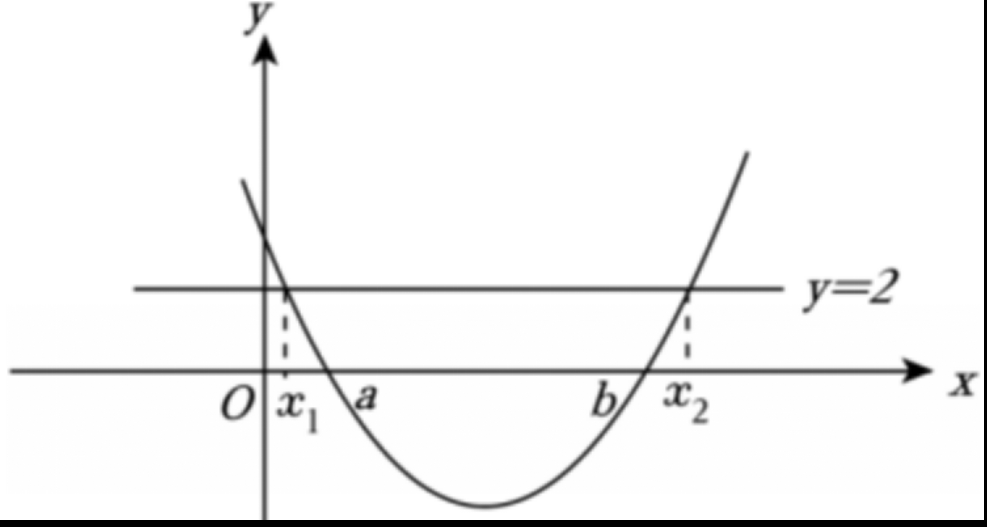
\includegraphics[width=0.42\textwidth]{figures/gao100_q16_parabola.png}
\end{center}
\step{所以数形结合得 $x_1<a<b<x_2$．故选 $B$.}
\solend
\fi

\end{enumerate}

\bigsec{三、解答题}

\begin{enumerate}
\setcounter{enumi}{16}

\item 已知集合 $A=\{x\mid3<x\leqslant6\}$，$B=\{x\mid m\leqslant x\leqslant2m+1\}$.

（1）若 $m=2$，求 $A\cap B$、$A\cup B$；

（2）若 $x\in B$ 是 $x\in A$ 的必要条件，求实数 $m$ 的取值范围.

\ansspace*[9]

\ifanswer
\solbegin
\stepm{（1）}{若 $m=2$，则 $B=\{x\mid2\leqslant x\leqslant5\}$，因为 $A=\{x\mid3<x\leqslant6\}$，}
\step{所以 $A\cap B=\{x\mid3<x\leqslant5\}$，$A\cup B=\{x\mid2\leqslant x\leqslant6\}$.}
\stepm{（2）}{因为 $x\in B$ 是 $x\in A$ 的必要条件，所以 $A\subseteq B$，}
\step{所以 $\begin{cases}m\leqslant3\\ 2m+1\geqslant6\end{cases}$，所以 $\dfrac52\leqslant m\leqslant3$，所以实数 $m$ 的取值范围为 $\left[\dfrac52,3\right]$.}
\solend
\fi

\item 求关于 $x$ 的不等式 $3ax^2-(3a+2)x+2<0\,(a\in R)$ 的解集.

\ansspace*[10]

\ifanswer
\solbegin
\step{当 $a=0$ 时，不等式化为 $-2x+2<0$，解得 $x>1$，}
\step{当 $a\neq0$ 时，方程 $3ax^2-(3a+2)x+2=0$ 的两根分别为 $1$，$\dfrac2{3a}$}
\step{当 $\dfrac2{3a}=1$，即 $a=\dfrac23$ 时，不等式化为 $(x-1)^2<0$，不等式无解，}
\step{当 $\dfrac2{3a}<1$，即 $a>\dfrac23$ 时，不等式解集为 $\left(\dfrac2{3a},1\right)$，}
\step{当 $0<a<\dfrac23$ 时，$\dfrac2{3a}>1$，不等式的解集为 $\left(1,\dfrac2{3a}\right)$，}
\step{当 $a<0$ 时，不等式的解集为 $\left(-\infty,\dfrac2{3a}\right)\cup(1,+\infty)$，}
\step{综上，当 $a=0$ 时，不等式的解集为 $(1,+\infty)$，}
\step{当 $a=\dfrac23$ 时，不等式的解集为 $\varnothing$，}
\step{当 $a>\dfrac23$ 时，不等式解集为 $\left(\dfrac2{3a},1\right)$，}
\step{当 $0<a<\dfrac23$ 时，不等式的解集为 $\left(1,\dfrac2{3a}\right)$，}
\step{当 $a<0$ 时，不等式的解集为 $\left(-\infty,\dfrac2{3a}\right)\cup(1,+\infty)$.}
\solend
\fi

\item 设对于任意实数 $x$，不等式 $\lvert x+1\rvert+\lvert x-1\rvert\geqslant m$ 恒成立.

（1）求 $m$ 的取值范围；

（2）当 $m$ 取最大值时，解关于 $x$ 的不等式 $\lvert x-3\rvert-2x\leqslant2m-2$.

\ansspace*[9]

\ifanswer
\solbegin
\stepm{（1）}{设函数 $f(x)=\lvert x+1\rvert+\lvert x-1\rvert$，则 $f(x)=\begin{cases}-2x,&x\leqslant-1\\ 2,&-1<x<1\\ 2x,&x\geqslant1\end{cases}$，}
\step{当 $x\leqslant-1$ 时，$f(x)$ 有最小值 2；}
\step{当 $-1<x<1$ 时，$f(x)=2$；}
\step{当 $x\geqslant1$ 时，$f(x)$ 有最小值 2；}
\step{因为对于任意实数 $x$，不等式 $\lvert x+1\rvert+\lvert x-1\rvert\geqslant m$ 恒成立，}
\step{所以 $m\leqslant2$，即 $m$ 的取值范围为 $(-\infty,2]$；}
\stepm{（2）}{由（1）得 $m$ 的最大值为 2，所以原不等式为 $\lvert x-3\rvert\leqslant2x+2$，}
\step{即 $-2x-2\leqslant x-3\leqslant2x+2$，解得 $x\geqslant\dfrac13$，}
\step{所以原不等式的解集为 $\left\{x\mid x\geqslant\dfrac13\right\}$.}
\solend
\fi

\item 某轮船公司的一艘轮船每小时花费的燃料费与轮船航行速度的平方成正比，比例系数为 $k$．轮船的最大速度为 18 海里/小时．当船速为 10 海里/小时，它的燃料费是每小时 120 元，其余航行运作费用（不论速度如何）总计是每小时 120 元．假定运行过程中轮船以速度 $v$ 匀速航行.

（1）求 $k$ 的值及每小时的最大总费用 $H$；

（2）求该轮船航行 100 海里的总费用 $W$（燃料费＋其余航行运作费用）的最小值.

\ansspace*[10]

\ifanswer
\solbegin
\stepm{（1）}{由题意，每小时燃料费为 $h(v)=kv^2$，$0<v\leqslant18$，}
\step{已知 $v=10$ 时，燃料费每小时 120 元，则 $k\cdot10^2=120$，得 $k=1.2$，}
\step{每小时总费用 $h(v)=kv^2+120=1.2v^2+120$，}
\step{$h(v)$ 是关于 $v$ 的增函数，$v$ 最大为 18，}
\step{所以 $H=h(18)=1.2\times18^2+120=508.8$ 元.}
\stepm{（2）}{航行时间 $t=\dfrac{100}v$ 小时，}
\step{$W(v)=h(v)\cdot t=(1.2v^2+120)\cdot\dfrac{100}v,0<v\leqslant18=120v+\dfrac{12000}v$，}
\step{利用均值不等式 $120v+\dfrac{12000}v\geqslant2\sqrt{120v\cdot\dfrac{12000}v}=2\times1200=2400$，}
\step{当且仅当 $120v=\dfrac{12000}v$，即 $v=10$ 时取等号，}
\step{$v=10\leqslant18$，在速度范围内，可取到等号，所以总费用最小值为 2400 元.}
\solend
\fi

\item 已知 $A$ 是 $R$ 的非空真子集，如果对任意 $x$、$y\in A$，都有 $x+y\in A$，$xy\in A$，则称 $A$ 是封闭集.

（1）判断集合 $B=\{0\}$，$C=\{-1,0,1\}$ 是否为封闭集，并说明理由；

（2）判断以下两个命题的真假，并说明理由；

命题 $p$：若非空集合 $A_1$、$A_2$ 是封闭集，则 $A_1\cup A_2$ 也是封闭集；

命题 $q$：非空集合 $A_1$、$A_2$ 是封闭集，则 $A_1\cap A_2\neq\varnothing$ 是 $A_1\cap A_2$ 是封闭集的充要条件；

（3）若非空集合 $A$ 是封闭集合，设全集为 $R$，求证：$A$ 的补集不是封闭集.

\ansspace*[13]

\ifanswer
\solbegin
\stepm{（1）}{$B=\{0\}$ 是封闭集，$C=\{-1,0,1\}$ 不是封闭集，理由如下：}
\step{对于集合 $B=\{0\}$，因为 $0+0=0\in B$，$0\times0=0\in B$，}
\step{所以 $B=\{0\}$ 是封闭集；}
\step{对于集合 $C=\{-1,0,1\}$，因为 $-1+(-1)=-2\notin C$，$1+1=2\notin C$，}
\step{所以集合 $C=\{-1,0,1\}$ 不是封闭集.}
\stepm{（2）}{命题 $p$ 是假命题，命题 $q$ 是真命题，理由如下：}
\step{对命题 $p$：令 $A_1=\{x\mid x=2k,k\in Z\}$，$A_2=\{x\mid x=3k,k\in Z\}$，}
\step{令 $x_1=2k_1$，$y_1=2k_2$，$k_1$、$k_2\in Z$，}
\step{则 $x_1+y_1=2(k_1+k_2)\in A_1$，$x_1y_1=2(2k_1k_2)\in A_1$，}
\step{因此集合 $A_1$ 是封闭集，同理集合 $A_2$ 也是封闭集，}
\step{取 $x_2=2$，$y_2=3$，则 $x_2$、$y_2\in(A_1\cup A_2)$，而 $x_2+y_2=5\notin(A_1\cup A_2)$，}
\step{因此集合 $A_1\cup A_2$ 不是封闭集，命题 $p$ 是假命题；}
\step{对于命题 $q$：若 $A_1\cap A_2\neq\varnothing$，不妨令 $a$、$b\in(A_1\cap A_2)$，}
\step{则有 $a$、$b\in A_1$，又集合 $A_1$ 是封闭集，则 $a+b\in A_1$，$ab\in A_1$，}
\step{同理 $a+b\in A_2$，$ab\in A_2$，因此 $a+b\in(A_1\cap A_2)$，$ab\in(A_1\cap A_2)$，}
\step{所以 $A_1\cap A_2$ 是封闭集；}
\step{反之，若 $A_1\cap A_2$ 是封闭集，则 $A_1\cap A_2$ 是非空集合，即 $A_1\cap A_2\neq\varnothing$，}
\step{所以 $A_1\cap A_2$ 是 $A_1\cap A_2$ 是封闭集的充要条件，命题 $q$ 是真命题.}
\stepm{（3）}{非空集合 $A$ 是封闭集合，当 $A=R$ 时，$\overline A=\varnothing$，因此 $\overline A$ 不是封闭集合；}
\step{当 $A\neq R$ 时，假设 $\overline A$ 是封闭集合，}
\step{设 $0\in A$，在 $\overline A$ 中任取一个 $x$，$x\neq0$，则 $-x\in A$，}
\step{否则 $-x\in\overline A$，此时 $x+(-x)=0\in\overline A$，与 $0\in A$ 矛盾，}
\step{因此 $(-x)^2\in A$，$x^2\in\overline A$，而 $(-x)^2=x^2$，与 $A\cap\overline A=\varnothing$ 矛盾，}
\step{则当 $0\in A$ 时，则 $\overline A$ 不是封闭集合，同理当 $0\in\overline A$ 时，$\overline A$ 不是封闭集合，}
\step{所以 $A$ 的补集不是封闭集.}
\solend
\fi

\end{enumerate}

\end{document}
"
% 紧凑版：xelatex "\def\iscompact{1}% 高一100_南洋中学_10月月考.tex
%   —— 高一上数学“2026-2027 年南洋中学高一上 10 月月考”（讲评版）
% 试卷版：xelatex 高一100_南洋中学_10月月考.tex
% 答案版：xelatex "\def\isanswer{1}\input{高一100_南洋中学_10月月考.tex}"
% 紧凑版：xelatex "\def\iscompact{1}\input{高一100_南洋中学_10月月考.tex}"
%
% 原始材料：微信公众号“魔都数学加油站”文章，连载“27学年高一100”；
% 原文标题“27学年高一100——2026-2027年上海市南洋中学高一上10月月考”；
% 原文链接：https://mp.weixin.qq.com/s/uXLyt6VHraW4hSpDwnZDuQ。
% 正文为 10 张 PNG 页（`原图/高一100_南洋中学_10月月考/01..10.png`），
% 尺寸混排（第 2、4—9 页为 4762×6735，第 1、3、10 页为 2560×3620），按页序读取。
%
% 篇幅与题号：原卷自第 3 题起编号（第 1、2 题不在原文内）。填空题 3—12（10 题）、
% 选择题 13—16（4 题）、解答题 17—21（5 题），共 19 题。
%
% 讲评版：全部 19 题均印【解析】，其中第 13—16 题的答案在解析末句
% “故选 $C$／$B$／$D$／$B$”（题干括号内未印答案）。第 16 题解析带一幅
% 抛物线与 $y=2$ 的示意图，自原图裁切、去粉色水印后转灰度，三版都出。
%
% 副标题：原卷未印副标题。本稿按内容标作“集合与常用逻辑用语、不等式”。
%
% 原卷笔误/存疑（均照录未改，正文对应处另有 % 注）：无。
%
% 与原卷的排版差异：
%   ① 原卷每题下直接印【解析】，本稿按全稿惯例将答案与解析置于答案版；
%   ② 原卷未印副标题，本稿补出；填空横线统一排 \blankline[4.4em]；
%   ③ 原卷数集记号排斜体 $R$、$Z$、$\mathit N$，本稿按全稿惯例改用 $\R$、$\Z$、$\N$；
%   ④ 解答题按惯例加 \ansspace；选择题括号排 \mbox{（\quad）}；
%   ⑤ 第 16 题的示意图原卷排在解析行右侧，本稿改排为解析后的居中图。
%
% 行数核对：逐题数 \step/\stepm 条数，合计 117 条（Q3：2；Q4：5；Q5：7；Q6：3；Q7：3；
% Q8：4；Q9：2；Q10：4；Q11：6；Q12：3；Q13：7；Q14：3；Q15：5；Q16：3；Q17：5；
% Q18：11；Q19：9；Q20：10；Q21：25）。全卷 19 题均印【解析】。
% 原卷解析的换行按语意合并，未逐行强拆。
%
\documentclass[a4paper,11pt]{article}
\usepackage{common}
\begin{document}

\examtitlest[7]{2026--2027 年南洋中学高一上 10 月月考}{集合与常用逻辑用语、不等式}

\bigsec{一、填空题}

\begin{enumerate}
\setcounter{enumi}{2}

\item 不等式 $\dfrac{x-6}{x+1}\geqslant0$ 的解集为\blankline[4.4em].

\ifanswer
\solbegin
\step{不等式 $\dfrac{x-6}{x+1}\geqslant0$ 等价于 $\begin{cases}(x-6)(x+1)\geqslant0\\ x+1\neq0\end{cases}$，即 $x<-1$ 或 $x\geqslant6$，}
\step{故解集为 $(-\infty,-1)\cup[6,+\infty)$.}
\solend
\fi

\item 已知关于 $x$ 的不等式 $ax^2+bx+c>0$ 的解集是 $(1,3)$，则关于 $x$ 的不等式 $ax^2-bx+c\leqslant0$ 的解集为\blankline[4.4em].

\ifanswer
\solbegin
\step{由已知得 $a<0$，且 $1$，$3$ 是方程 $ax^2+bx+c=0$ 的根，}
\step{所以 $\begin{cases}1+3=-\dfrac ba\\[2pt] 1\times3=\dfrac ca\end{cases}$，所以 $\begin{cases}b=-4a\\ c=3a\end{cases}$，}
\step{所以 $ax^2-bx+c\leqslant0$ 可变形为 $ax^2+4ax+3a\leqslant0$，}
\step{因为 $a<0$，所以 $x^2+4x+3\geqslant0$，解得 $x\leqslant-3$ 或 $x\geqslant-1$，}
\step{所以不等式的解集为 $(-\infty,-3]\cup[-1,+\infty)$.}
\solend
\fi

\item 不等式 $\lvert x+2\rvert+\lvert 2x-1\rvert\geqslant3$ 的解集为\blankline[4.4em].

\ifanswer
\solbegin
\step{当 $x\leqslant-2$ 时，$x+2\leqslant0$，$2x-1<0$，}
\step{所以 $\lvert x+2\rvert+\lvert 2x-1\rvert=-x-2-2x+1\geqslant3$，解得 $x\leqslant-\dfrac43$；}
\step{当 $-2<x<\dfrac12$ 时，$x+2>0$，$2x-1<0$，}
\step{所以 $\lvert x+2\rvert+\lvert 2x-1\rvert=x+2-2x+1\geqslant3$，解得 $x\leqslant0$；}
\step{当 $x\geqslant\dfrac12$ 时，$x+2>0$，$2x-1\geqslant0$，}
\step{所以 $\lvert x+2\rvert+\lvert 2x-1\rvert=x+2+2x-1\geqslant3$，解得 $x\geqslant\dfrac23$；}
\step{所以原不等式的解集为 $\left\{x\mid x\leqslant0\right.$ 或 $\left.x\geqslant\dfrac23\right\}$.}
\solend
\fi

\item 若正数 $x$、$y$ 满足 $x+2y=2$，则 $\dfrac1x+\dfrac2y$ 的最小值是\blankline[4.4em].

\ifanswer
\solbegin
\step{因为 $x>0$，$y>0$，且 $x+2y=2$，}
\step{所以 $\dfrac1x+\dfrac2y=\dfrac12\left(\dfrac1x+\dfrac2y\right)(x+2y)=\dfrac12\left(5+\dfrac{2y}x+\dfrac{2x}y\right)\geqslant\dfrac12\left(5+2\sqrt{\dfrac{2y}x\cdot\dfrac{2x}y}\right)=\dfrac92$.}
\step{当且仅当 $\begin{cases}x+2y=2\\ \dfrac{2y}x=\dfrac{2x}y\end{cases}$，即 $x=y=\dfrac23$ 时取等号，故最小值为 $\dfrac92$.}
\solend
\fi

\item 已知 $\alpha:x\leqslant2$ 或 $x>3$，$\beta:x\leqslant m+5$ 或 $x>-m$，若 $\alpha$ 是 $\beta$ 的必要非充分条件，则实数 $m$ 的取值范围是\blankline[4.4em].

\ifanswer
\solbegin
\step{设 $A=\{x\mid x\leqslant2$ 或 $x>3\}$，$B=\{x\mid x\leqslant m+5$ 或 $x>-m\}$，则 $B\subset A$，}
\step{则 $m+5\leqslant2$ 且 $-m\geqslant3$（等号不能同时取得），则 $m<-3$，}
\step{则实数 $m$ 的取值范围是 $(-\infty,-3)$.}
\solend
\fi

\item 已知集合 $A=\{x\mid-1\leqslant x\leqslant3\}$，$B=\{x\mid ax+1>0\}$ 满足 $A\subseteq B$，则实数 $a$ 的取值范围为\blankline[4.4em].

\ifanswer
\solbegin
\step{当 $a=0$ 时，$B=R$，显然符合题意，}
\step{当 $a>0$ 时，$B=\left\{x\mid x>-\dfrac1a\right\}$，则 $-\dfrac1a<-1$，解得 $a<1$，所以 $0<a<1$，}
\step{当 $a<0$ 时，$B=\left\{x\mid x<-\dfrac1a\right\}$，则 $-\dfrac1a>3$，解得 $a>-\dfrac13$，所以 $-\dfrac13<a<0$，}
\step{综上所述，实数 $a$ 的取值范围为 $\left(-\dfrac13,1\right)$.}
\solend
\fi

\item 设集合 $A=\{x\mid3x-1<m\}$，若 $1\in A$ 且 $2\notin A$，则实数 $m$ 的取值范围是\blankline[4.4em].

\ifanswer
\solbegin
\step{因为集合 $A=\{x\mid3x-1<m\}$，若 $1\in A$ 且 $2\notin A$，}
\step{则 $3\times1-1<m$ 且 $3\times2-1\geqslant m$，解得 $2<m\leqslant5$.}
\solend
\fi

\item 若 $M=\left\{x\mid x=m+\dfrac16,m\in Z\right\},N=\left\{x\mid x=\dfrac n2-\dfrac13,n\in Z\right\}$，\newline $P=\left\{x\mid x=\dfrac p2+\dfrac16,p\in Z\right\}$，则 $M$、$N$、$P$ 的关系为\blankline[4.4em].

\ifanswer
\solbegin
\step{$M=\left\{x\mid x=m+\dfrac16=\dfrac{6m+1}6=\dfrac{3\cdot2m+1}6,m\in Z\right\}$，}
\step{$N=\left\{x\mid x=\dfrac n2-\dfrac13=\dfrac{3(n-1)+1}6,n\in Z\right\}=\left\{x\mid x=\dfrac{3k+1}6,k\in Z\right\}$，}
\step{$P=\left\{x\mid x=\dfrac p2+\dfrac16=\dfrac{3p+1}6,p\in Z\right\}$，}
\step{故 $M\subset N=P$.}
\solend
\fi

\item 已知命题 $p:x<-2$ 或 $x>3$，命题 $q:x<3m+1$ 或 $x>m+2$，若 $p$ 是 $q$ 的充分非必要条件，则实数 $m$ 的取值范围是\blankline[4.4em].

\ifanswer
\solbegin
\step{设 $A=\{x\mid x<-2$ 或 $x>3\}$，$B=\{x\mid x<3m+1$ 或 $x>m+2\}$，}
\step{若 $p$ 是 $q$ 的充分非必要条件，则 $A\subset B$，}
\step{当 $3m+1\geqslant m+2$，即 $m\geqslant\dfrac12$ 时，显然有 $A\subset B$，}
\step{当 $3m+1<m+2$，即 $m<\dfrac12$ 时，}
\step{由 $A\subset B$，则 $\begin{cases}m+2\leqslant3\\ 3m+1\geqslant-2\end{cases}$（等号不同时成立），即 $-1\leqslant m<\dfrac12$.}
\step{综上，实数 $m$ 的取值范围是 $[-1,+\infty)$.}
\solend
\fi

\item 对于一个有限集 $A$，一般都可以找到两个非空数集 $A_1$ 和 $A_2$，满足 $A_1\cap A_2=\varnothing$，且 $A_1\cup A_2=A$，记集合 $\{A_1,A_2\}$ 为 $A$ 的一个“划分集”．若 $A$ 中有 $n(n\geqslant2,n\in\N)$ 个元素，则不同的“划分集”共有\blankline[4.4em]个(用含 $n$ 的表达式填空).

\ifanswer
\solbegin
\step{集合中的每个元素都有属于 $A_1$ 或属于 $A_2$ 两种情况，故共有 $2^n$ 种情况，}
\step{排除全都属于 $A_1$ 或 $A_2$ 的两种情况，考虑对称情况，}
\step{故不同的“划分集”共有 $\dfrac12(2^n-2)=2^{n-1}-1$ 个.}
\solend
\fi

\end{enumerate}

\bigsec{二、选择题}

\begin{enumerate}
\setcounter{enumi}{12}

\item 下列命题中正确的\mbox{（\quad）}

\keepwithprev
A. $\varnothing$ 与 $\{0\}$ 表示同一个集合

B. 方程 $\{x\mid(x-2)^2(x-3)=0\}$ 的所有解的集合可表示为 $\{2,2,3\}$

C. 由 3，4，5 组成的集合可表示为 $\{3,4,5\}$ 或 $\{4,5,3\}$

D. 很小的实数可以构成集合.

\ifanswer
\solbegin
\step{对于 $A$，$\{0\}$ 中有一个元素 0，$\varnothing$ 中无任何元素，故 $\varnothing$ 与 $\{0\}$ 不是同一个集合，}
\step{故 $A$ 错误；}
\step{对于 $B$，$\{2,2,3\}$ 不满足集合元素的互异性，故 $B$ 错误；}
\step{对于 $C$，由集合的无序性，得由 3，4，5 组成的集合可表示为 $\{3,4,5\}$ 或 $\{4,5,3\}$，}
\step{故 $C$ 正确；}
\step{对于 $D$，由集合的确定性，很小的实数不能构成集合，故 $D$ 错误.}
\step{故选 $C$.}
\solend
\fi

\item 已知 $a\in R$，则“$\dfrac1a<1$”是“$a>1$”的\mbox{（\quad）}条件.

\keepwithprev
A. 充分非必要\qquad B. 必要非充分

C. 充要\qquad D. 既非充分又非必要

\ifanswer
\solbegin
\step{解 $\dfrac1a<1$，得 $a<0$ 或 $a>1$，}
\step{由 $a<0$ 或 $a>1$ 得不出 $a>1$，由 $a>1$ 得出 $a<0$ 或 $a>1$，}
\step{所以“$\dfrac1a<1$”是“$a>1$”的必要不充分条件．故选 $B$.}
\solend
\fi

\item 若命题“存在 $x_0\in R$ 使得 $ax_0^2+2ax_0+1\leqslant0$”是假命题，则实数 $a$ 的取值范围为\mbox{（\quad）}

\keepwithprev
A. $a<0$ 或 $a\geqslant1$\qquad B. $a\leqslant0$ 或 $a\geqslant1$\qquad C. $0<a<1$\qquad D. $0\leqslant a<1$

\ifanswer
\solbegin
\step{命题“存在 $x_0\in R$ 使得 $ax_0^2+2ax_0+1\leqslant0$”是假命题，}
\step{则 $\forall x\in R$，$ax^2+2ax+1>0$ 恒成立，}
\step{当 $a=0$ 时，满足题意，}
\step{当 $a\neq0$ 时，$\begin{cases}a>0\\ \Delta=4a^2-4a<0\end{cases}$，解得 $0<a<1$，}
\step{综上所述，实数 $a$ 的取值范围为 $\{a\mid0\leqslant a<1\}$．故选 $D$.}
\solend
\fi

\item 已知实数 $a<b$，关于 $x$ 的不等式 $x^2-(a+b)x+ab-2<0$ 的解集为 $(x_1,x_2)$，则实数 $a$、$b$、$x_1$、$x_2$ 从小到大的排列是\mbox{（\quad）}

\keepwithprev
A. $a<x_1<x_2<b$\qquad B. $x_1<a<b<x_2$\qquad C. $a<x_1<b<x_2$\qquad D. $x_1<a<x_2<b$

\ifanswer
\solbegin
\step{因为实数 $a<b$，不等式 $x^2-(a+b)x+ab-2<0$ 可化为 $(x-a)(x-b)<2$，}
\step{又其解集为 $(x_1,x_2)$，所以作出 $y=(x-a)(x-b)$ 与 $y=2$ 的图象如下：}
\begin{center}
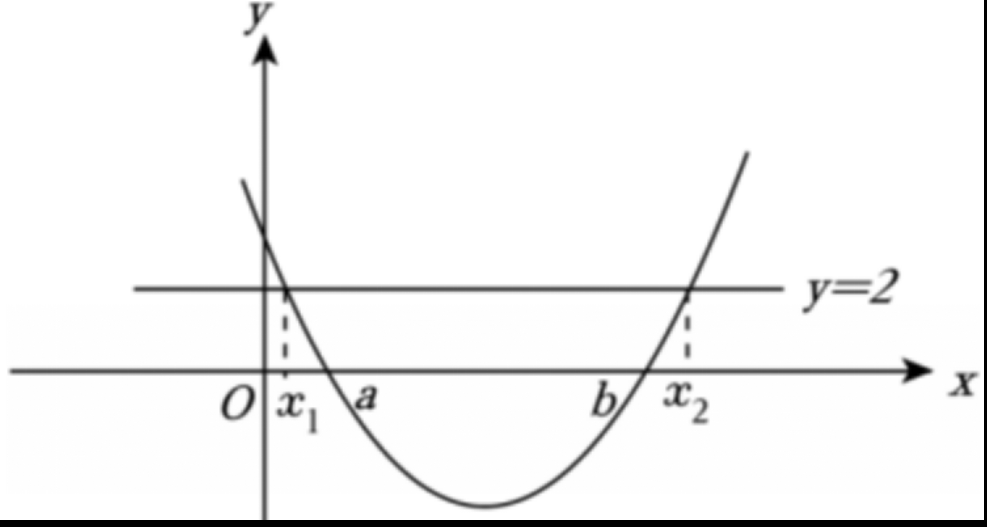
\includegraphics[width=0.42\textwidth]{figures/gao100_q16_parabola.png}
\end{center}
\step{所以数形结合得 $x_1<a<b<x_2$．故选 $B$.}
\solend
\fi

\end{enumerate}

\bigsec{三、解答题}

\begin{enumerate}
\setcounter{enumi}{16}

\item 已知集合 $A=\{x\mid3<x\leqslant6\}$，$B=\{x\mid m\leqslant x\leqslant2m+1\}$.

（1）若 $m=2$，求 $A\cap B$、$A\cup B$；

（2）若 $x\in B$ 是 $x\in A$ 的必要条件，求实数 $m$ 的取值范围.

\ansspace*[9]

\ifanswer
\solbegin
\stepm{（1）}{若 $m=2$，则 $B=\{x\mid2\leqslant x\leqslant5\}$，因为 $A=\{x\mid3<x\leqslant6\}$，}
\step{所以 $A\cap B=\{x\mid3<x\leqslant5\}$，$A\cup B=\{x\mid2\leqslant x\leqslant6\}$.}
\stepm{（2）}{因为 $x\in B$ 是 $x\in A$ 的必要条件，所以 $A\subseteq B$，}
\step{所以 $\begin{cases}m\leqslant3\\ 2m+1\geqslant6\end{cases}$，所以 $\dfrac52\leqslant m\leqslant3$，所以实数 $m$ 的取值范围为 $\left[\dfrac52,3\right]$.}
\solend
\fi

\item 求关于 $x$ 的不等式 $3ax^2-(3a+2)x+2<0\,(a\in R)$ 的解集.

\ansspace*[10]

\ifanswer
\solbegin
\step{当 $a=0$ 时，不等式化为 $-2x+2<0$，解得 $x>1$，}
\step{当 $a\neq0$ 时，方程 $3ax^2-(3a+2)x+2=0$ 的两根分别为 $1$，$\dfrac2{3a}$}
\step{当 $\dfrac2{3a}=1$，即 $a=\dfrac23$ 时，不等式化为 $(x-1)^2<0$，不等式无解，}
\step{当 $\dfrac2{3a}<1$，即 $a>\dfrac23$ 时，不等式解集为 $\left(\dfrac2{3a},1\right)$，}
\step{当 $0<a<\dfrac23$ 时，$\dfrac2{3a}>1$，不等式的解集为 $\left(1,\dfrac2{3a}\right)$，}
\step{当 $a<0$ 时，不等式的解集为 $\left(-\infty,\dfrac2{3a}\right)\cup(1,+\infty)$，}
\step{综上，当 $a=0$ 时，不等式的解集为 $(1,+\infty)$，}
\step{当 $a=\dfrac23$ 时，不等式的解集为 $\varnothing$，}
\step{当 $a>\dfrac23$ 时，不等式解集为 $\left(\dfrac2{3a},1\right)$，}
\step{当 $0<a<\dfrac23$ 时，不等式的解集为 $\left(1,\dfrac2{3a}\right)$，}
\step{当 $a<0$ 时，不等式的解集为 $\left(-\infty,\dfrac2{3a}\right)\cup(1,+\infty)$.}
\solend
\fi

\item 设对于任意实数 $x$，不等式 $\lvert x+1\rvert+\lvert x-1\rvert\geqslant m$ 恒成立.

（1）求 $m$ 的取值范围；

（2）当 $m$ 取最大值时，解关于 $x$ 的不等式 $\lvert x-3\rvert-2x\leqslant2m-2$.

\ansspace*[9]

\ifanswer
\solbegin
\stepm{（1）}{设函数 $f(x)=\lvert x+1\rvert+\lvert x-1\rvert$，则 $f(x)=\begin{cases}-2x,&x\leqslant-1\\ 2,&-1<x<1\\ 2x,&x\geqslant1\end{cases}$，}
\step{当 $x\leqslant-1$ 时，$f(x)$ 有最小值 2；}
\step{当 $-1<x<1$ 时，$f(x)=2$；}
\step{当 $x\geqslant1$ 时，$f(x)$ 有最小值 2；}
\step{因为对于任意实数 $x$，不等式 $\lvert x+1\rvert+\lvert x-1\rvert\geqslant m$ 恒成立，}
\step{所以 $m\leqslant2$，即 $m$ 的取值范围为 $(-\infty,2]$；}
\stepm{（2）}{由（1）得 $m$ 的最大值为 2，所以原不等式为 $\lvert x-3\rvert\leqslant2x+2$，}
\step{即 $-2x-2\leqslant x-3\leqslant2x+2$，解得 $x\geqslant\dfrac13$，}
\step{所以原不等式的解集为 $\left\{x\mid x\geqslant\dfrac13\right\}$.}
\solend
\fi

\item 某轮船公司的一艘轮船每小时花费的燃料费与轮船航行速度的平方成正比，比例系数为 $k$．轮船的最大速度为 18 海里/小时．当船速为 10 海里/小时，它的燃料费是每小时 120 元，其余航行运作费用（不论速度如何）总计是每小时 120 元．假定运行过程中轮船以速度 $v$ 匀速航行.

（1）求 $k$ 的值及每小时的最大总费用 $H$；

（2）求该轮船航行 100 海里的总费用 $W$（燃料费＋其余航行运作费用）的最小值.

\ansspace*[10]

\ifanswer
\solbegin
\stepm{（1）}{由题意，每小时燃料费为 $h(v)=kv^2$，$0<v\leqslant18$，}
\step{已知 $v=10$ 时，燃料费每小时 120 元，则 $k\cdot10^2=120$，得 $k=1.2$，}
\step{每小时总费用 $h(v)=kv^2+120=1.2v^2+120$，}
\step{$h(v)$ 是关于 $v$ 的增函数，$v$ 最大为 18，}
\step{所以 $H=h(18)=1.2\times18^2+120=508.8$ 元.}
\stepm{（2）}{航行时间 $t=\dfrac{100}v$ 小时，}
\step{$W(v)=h(v)\cdot t=(1.2v^2+120)\cdot\dfrac{100}v,0<v\leqslant18=120v+\dfrac{12000}v$，}
\step{利用均值不等式 $120v+\dfrac{12000}v\geqslant2\sqrt{120v\cdot\dfrac{12000}v}=2\times1200=2400$，}
\step{当且仅当 $120v=\dfrac{12000}v$，即 $v=10$ 时取等号，}
\step{$v=10\leqslant18$，在速度范围内，可取到等号，所以总费用最小值为 2400 元.}
\solend
\fi

\item 已知 $A$ 是 $R$ 的非空真子集，如果对任意 $x$、$y\in A$，都有 $x+y\in A$，$xy\in A$，则称 $A$ 是封闭集.

（1）判断集合 $B=\{0\}$，$C=\{-1,0,1\}$ 是否为封闭集，并说明理由；

（2）判断以下两个命题的真假，并说明理由；

命题 $p$：若非空集合 $A_1$、$A_2$ 是封闭集，则 $A_1\cup A_2$ 也是封闭集；

命题 $q$：非空集合 $A_1$、$A_2$ 是封闭集，则 $A_1\cap A_2\neq\varnothing$ 是 $A_1\cap A_2$ 是封闭集的充要条件；

（3）若非空集合 $A$ 是封闭集合，设全集为 $R$，求证：$A$ 的补集不是封闭集.

\ansspace*[13]

\ifanswer
\solbegin
\stepm{（1）}{$B=\{0\}$ 是封闭集，$C=\{-1,0,1\}$ 不是封闭集，理由如下：}
\step{对于集合 $B=\{0\}$，因为 $0+0=0\in B$，$0\times0=0\in B$，}
\step{所以 $B=\{0\}$ 是封闭集；}
\step{对于集合 $C=\{-1,0,1\}$，因为 $-1+(-1)=-2\notin C$，$1+1=2\notin C$，}
\step{所以集合 $C=\{-1,0,1\}$ 不是封闭集.}
\stepm{（2）}{命题 $p$ 是假命题，命题 $q$ 是真命题，理由如下：}
\step{对命题 $p$：令 $A_1=\{x\mid x=2k,k\in Z\}$，$A_2=\{x\mid x=3k,k\in Z\}$，}
\step{令 $x_1=2k_1$，$y_1=2k_2$，$k_1$、$k_2\in Z$，}
\step{则 $x_1+y_1=2(k_1+k_2)\in A_1$，$x_1y_1=2(2k_1k_2)\in A_1$，}
\step{因此集合 $A_1$ 是封闭集，同理集合 $A_2$ 也是封闭集，}
\step{取 $x_2=2$，$y_2=3$，则 $x_2$、$y_2\in(A_1\cup A_2)$，而 $x_2+y_2=5\notin(A_1\cup A_2)$，}
\step{因此集合 $A_1\cup A_2$ 不是封闭集，命题 $p$ 是假命题；}
\step{对于命题 $q$：若 $A_1\cap A_2\neq\varnothing$，不妨令 $a$、$b\in(A_1\cap A_2)$，}
\step{则有 $a$、$b\in A_1$，又集合 $A_1$ 是封闭集，则 $a+b\in A_1$，$ab\in A_1$，}
\step{同理 $a+b\in A_2$，$ab\in A_2$，因此 $a+b\in(A_1\cap A_2)$，$ab\in(A_1\cap A_2)$，}
\step{所以 $A_1\cap A_2$ 是封闭集；}
\step{反之，若 $A_1\cap A_2$ 是封闭集，则 $A_1\cap A_2$ 是非空集合，即 $A_1\cap A_2\neq\varnothing$，}
\step{所以 $A_1\cap A_2$ 是 $A_1\cap A_2$ 是封闭集的充要条件，命题 $q$ 是真命题.}
\stepm{（3）}{非空集合 $A$ 是封闭集合，当 $A=R$ 时，$\overline A=\varnothing$，因此 $\overline A$ 不是封闭集合；}
\step{当 $A\neq R$ 时，假设 $\overline A$ 是封闭集合，}
\step{设 $0\in A$，在 $\overline A$ 中任取一个 $x$，$x\neq0$，则 $-x\in A$，}
\step{否则 $-x\in\overline A$，此时 $x+(-x)=0\in\overline A$，与 $0\in A$ 矛盾，}
\step{因此 $(-x)^2\in A$，$x^2\in\overline A$，而 $(-x)^2=x^2$，与 $A\cap\overline A=\varnothing$ 矛盾，}
\step{则当 $0\in A$ 时，则 $\overline A$ 不是封闭集合，同理当 $0\in\overline A$ 时，$\overline A$ 不是封闭集合，}
\step{所以 $A$ 的补集不是封闭集.}
\solend
\fi

\end{enumerate}

\end{document}
"
%
% 原始材料：微信公众号“魔都数学加油站”文章，连载“27学年高一100”；
% 原文标题“27学年高一100——2026-2027年上海市南洋中学高一上10月月考”；
% 原文链接：https://mp.weixin.qq.com/s/uXLyt6VHraW4hSpDwnZDuQ。
% 正文为 10 张 PNG 页（`原图/高一100_南洋中学_10月月考/01..10.png`），
% 尺寸混排（第 2、4—9 页为 4762×6735，第 1、3、10 页为 2560×3620），按页序读取。
%
% 篇幅与题号：原卷自第 3 题起编号（第 1、2 题不在原文内）。填空题 3—12（10 题）、
% 选择题 13—16（4 题）、解答题 17—21（5 题），共 19 题。
%
% 讲评版：全部 19 题均印【解析】，其中第 13—16 题的答案在解析末句
% “故选 $C$／$B$／$D$／$B$”（题干括号内未印答案）。第 16 题解析带一幅
% 抛物线与 $y=2$ 的示意图，自原图裁切、去粉色水印后转灰度，三版都出。
%
% 副标题：原卷未印副标题。本稿按内容标作“集合与常用逻辑用语、不等式”。
%
% 原卷笔误/存疑（均照录未改，正文对应处另有 % 注）：无。
%
% 与原卷的排版差异：
%   ① 原卷每题下直接印【解析】，本稿按全稿惯例将答案与解析置于答案版；
%   ② 原卷未印副标题，本稿补出；填空横线统一排 \blankline[4.4em]；
%   ③ 原卷数集记号排斜体 $R$、$Z$、$\mathit N$，本稿按全稿惯例改用 $\R$、$\Z$、$\N$；
%   ④ 解答题按惯例加 \ansspace；选择题括号排 \mbox{（\quad）}；
%   ⑤ 第 16 题的示意图原卷排在解析行右侧，本稿改排为解析后的居中图。
%
% 行数核对：逐题数 \step/\stepm 条数，合计 117 条（Q3：2；Q4：5；Q5：7；Q6：3；Q7：3；
% Q8：4；Q9：2；Q10：4；Q11：6；Q12：3；Q13：7；Q14：3；Q15：5；Q16：3；Q17：5；
% Q18：11；Q19：9；Q20：10；Q21：25）。全卷 19 题均印【解析】。
% 原卷解析的换行按语意合并，未逐行强拆。
%
\documentclass[a4paper,11pt]{article}
\usepackage{common}
\begin{document}

\examtitlest[7]{2026--2027 年南洋中学高一上 10 月月考}{集合与常用逻辑用语、不等式}

\bigsec{一、填空题}

\begin{enumerate}
\setcounter{enumi}{2}

\item 不等式 $\dfrac{x-6}{x+1}\geqslant0$ 的解集为\blankline[4.4em].

\ifanswer
\solbegin
\step{不等式 $\dfrac{x-6}{x+1}\geqslant0$ 等价于 $\begin{cases}(x-6)(x+1)\geqslant0\\ x+1\neq0\end{cases}$，即 $x<-1$ 或 $x\geqslant6$，}
\step{故解集为 $(-\infty,-1)\cup[6,+\infty)$.}
\solend
\fi

\item 已知关于 $x$ 的不等式 $ax^2+bx+c>0$ 的解集是 $(1,3)$，则关于 $x$ 的不等式 $ax^2-bx+c\leqslant0$ 的解集为\blankline[4.4em].

\ifanswer
\solbegin
\step{由已知得 $a<0$，且 $1$，$3$ 是方程 $ax^2+bx+c=0$ 的根，}
\step{所以 $\begin{cases}1+3=-\dfrac ba\\[2pt] 1\times3=\dfrac ca\end{cases}$，所以 $\begin{cases}b=-4a\\ c=3a\end{cases}$，}
\step{所以 $ax^2-bx+c\leqslant0$ 可变形为 $ax^2+4ax+3a\leqslant0$，}
\step{因为 $a<0$，所以 $x^2+4x+3\geqslant0$，解得 $x\leqslant-3$ 或 $x\geqslant-1$，}
\step{所以不等式的解集为 $(-\infty,-3]\cup[-1,+\infty)$.}
\solend
\fi

\item 不等式 $\lvert x+2\rvert+\lvert 2x-1\rvert\geqslant3$ 的解集为\blankline[4.4em].

\ifanswer
\solbegin
\step{当 $x\leqslant-2$ 时，$x+2\leqslant0$，$2x-1<0$，}
\step{所以 $\lvert x+2\rvert+\lvert 2x-1\rvert=-x-2-2x+1\geqslant3$，解得 $x\leqslant-\dfrac43$；}
\step{当 $-2<x<\dfrac12$ 时，$x+2>0$，$2x-1<0$，}
\step{所以 $\lvert x+2\rvert+\lvert 2x-1\rvert=x+2-2x+1\geqslant3$，解得 $x\leqslant0$；}
\step{当 $x\geqslant\dfrac12$ 时，$x+2>0$，$2x-1\geqslant0$，}
\step{所以 $\lvert x+2\rvert+\lvert 2x-1\rvert=x+2+2x-1\geqslant3$，解得 $x\geqslant\dfrac23$；}
\step{所以原不等式的解集为 $\left\{x\mid x\leqslant0\right.$ 或 $\left.x\geqslant\dfrac23\right\}$.}
\solend
\fi

\item 若正数 $x$、$y$ 满足 $x+2y=2$，则 $\dfrac1x+\dfrac2y$ 的最小值是\blankline[4.4em].

\ifanswer
\solbegin
\step{因为 $x>0$，$y>0$，且 $x+2y=2$，}
\step{所以 $\dfrac1x+\dfrac2y=\dfrac12\left(\dfrac1x+\dfrac2y\right)(x+2y)=\dfrac12\left(5+\dfrac{2y}x+\dfrac{2x}y\right)\geqslant\dfrac12\left(5+2\sqrt{\dfrac{2y}x\cdot\dfrac{2x}y}\right)=\dfrac92$.}
\step{当且仅当 $\begin{cases}x+2y=2\\ \dfrac{2y}x=\dfrac{2x}y\end{cases}$，即 $x=y=\dfrac23$ 时取等号，故最小值为 $\dfrac92$.}
\solend
\fi

\item 已知 $\alpha:x\leqslant2$ 或 $x>3$，$\beta:x\leqslant m+5$ 或 $x>-m$，若 $\alpha$ 是 $\beta$ 的必要非充分条件，则实数 $m$ 的取值范围是\blankline[4.4em].

\ifanswer
\solbegin
\step{设 $A=\{x\mid x\leqslant2$ 或 $x>3\}$，$B=\{x\mid x\leqslant m+5$ 或 $x>-m\}$，则 $B\subset A$，}
\step{则 $m+5\leqslant2$ 且 $-m\geqslant3$（等号不能同时取得），则 $m<-3$，}
\step{则实数 $m$ 的取值范围是 $(-\infty,-3)$.}
\solend
\fi

\item 已知集合 $A=\{x\mid-1\leqslant x\leqslant3\}$，$B=\{x\mid ax+1>0\}$ 满足 $A\subseteq B$，则实数 $a$ 的取值范围为\blankline[4.4em].

\ifanswer
\solbegin
\step{当 $a=0$ 时，$B=R$，显然符合题意，}
\step{当 $a>0$ 时，$B=\left\{x\mid x>-\dfrac1a\right\}$，则 $-\dfrac1a<-1$，解得 $a<1$，所以 $0<a<1$，}
\step{当 $a<0$ 时，$B=\left\{x\mid x<-\dfrac1a\right\}$，则 $-\dfrac1a>3$，解得 $a>-\dfrac13$，所以 $-\dfrac13<a<0$，}
\step{综上所述，实数 $a$ 的取值范围为 $\left(-\dfrac13,1\right)$.}
\solend
\fi

\item 设集合 $A=\{x\mid3x-1<m\}$，若 $1\in A$ 且 $2\notin A$，则实数 $m$ 的取值范围是\blankline[4.4em].

\ifanswer
\solbegin
\step{因为集合 $A=\{x\mid3x-1<m\}$，若 $1\in A$ 且 $2\notin A$，}
\step{则 $3\times1-1<m$ 且 $3\times2-1\geqslant m$，解得 $2<m\leqslant5$.}
\solend
\fi

\item 若 $M=\left\{x\mid x=m+\dfrac16,m\in Z\right\},N=\left\{x\mid x=\dfrac n2-\dfrac13,n\in Z\right\}$，\newline $P=\left\{x\mid x=\dfrac p2+\dfrac16,p\in Z\right\}$，则 $M$、$N$、$P$ 的关系为\blankline[4.4em].

\ifanswer
\solbegin
\step{$M=\left\{x\mid x=m+\dfrac16=\dfrac{6m+1}6=\dfrac{3\cdot2m+1}6,m\in Z\right\}$，}
\step{$N=\left\{x\mid x=\dfrac n2-\dfrac13=\dfrac{3(n-1)+1}6,n\in Z\right\}=\left\{x\mid x=\dfrac{3k+1}6,k\in Z\right\}$，}
\step{$P=\left\{x\mid x=\dfrac p2+\dfrac16=\dfrac{3p+1}6,p\in Z\right\}$，}
\step{故 $M\subset N=P$.}
\solend
\fi

\item 已知命题 $p:x<-2$ 或 $x>3$，命题 $q:x<3m+1$ 或 $x>m+2$，若 $p$ 是 $q$ 的充分非必要条件，则实数 $m$ 的取值范围是\blankline[4.4em].

\ifanswer
\solbegin
\step{设 $A=\{x\mid x<-2$ 或 $x>3\}$，$B=\{x\mid x<3m+1$ 或 $x>m+2\}$，}
\step{若 $p$ 是 $q$ 的充分非必要条件，则 $A\subset B$，}
\step{当 $3m+1\geqslant m+2$，即 $m\geqslant\dfrac12$ 时，显然有 $A\subset B$，}
\step{当 $3m+1<m+2$，即 $m<\dfrac12$ 时，}
\step{由 $A\subset B$，则 $\begin{cases}m+2\leqslant3\\ 3m+1\geqslant-2\end{cases}$（等号不同时成立），即 $-1\leqslant m<\dfrac12$.}
\step{综上，实数 $m$ 的取值范围是 $[-1,+\infty)$.}
\solend
\fi

\item 对于一个有限集 $A$，一般都可以找到两个非空数集 $A_1$ 和 $A_2$，满足 $A_1\cap A_2=\varnothing$，且 $A_1\cup A_2=A$，记集合 $\{A_1,A_2\}$ 为 $A$ 的一个“划分集”．若 $A$ 中有 $n(n\geqslant2,n\in\N)$ 个元素，则不同的“划分集”共有\blankline[4.4em]个(用含 $n$ 的表达式填空).

\ifanswer
\solbegin
\step{集合中的每个元素都有属于 $A_1$ 或属于 $A_2$ 两种情况，故共有 $2^n$ 种情况，}
\step{排除全都属于 $A_1$ 或 $A_2$ 的两种情况，考虑对称情况，}
\step{故不同的“划分集”共有 $\dfrac12(2^n-2)=2^{n-1}-1$ 个.}
\solend
\fi

\end{enumerate}

\bigsec{二、选择题}

\begin{enumerate}
\setcounter{enumi}{12}

\item 下列命题中正确的\mbox{（\quad）}

\keepwithprev
A. $\varnothing$ 与 $\{0\}$ 表示同一个集合

B. 方程 $\{x\mid(x-2)^2(x-3)=0\}$ 的所有解的集合可表示为 $\{2,2,3\}$

C. 由 3，4，5 组成的集合可表示为 $\{3,4,5\}$ 或 $\{4,5,3\}$

D. 很小的实数可以构成集合.

\ifanswer
\solbegin
\step{对于 $A$，$\{0\}$ 中有一个元素 0，$\varnothing$ 中无任何元素，故 $\varnothing$ 与 $\{0\}$ 不是同一个集合，}
\step{故 $A$ 错误；}
\step{对于 $B$，$\{2,2,3\}$ 不满足集合元素的互异性，故 $B$ 错误；}
\step{对于 $C$，由集合的无序性，得由 3，4，5 组成的集合可表示为 $\{3,4,5\}$ 或 $\{4,5,3\}$，}
\step{故 $C$ 正确；}
\step{对于 $D$，由集合的确定性，很小的实数不能构成集合，故 $D$ 错误.}
\step{故选 $C$.}
\solend
\fi

\item 已知 $a\in R$，则“$\dfrac1a<1$”是“$a>1$”的\mbox{（\quad）}条件.

\keepwithprev
A. 充分非必要\qquad B. 必要非充分

C. 充要\qquad D. 既非充分又非必要

\ifanswer
\solbegin
\step{解 $\dfrac1a<1$，得 $a<0$ 或 $a>1$，}
\step{由 $a<0$ 或 $a>1$ 得不出 $a>1$，由 $a>1$ 得出 $a<0$ 或 $a>1$，}
\step{所以“$\dfrac1a<1$”是“$a>1$”的必要不充分条件．故选 $B$.}
\solend
\fi

\item 若命题“存在 $x_0\in R$ 使得 $ax_0^2+2ax_0+1\leqslant0$”是假命题，则实数 $a$ 的取值范围为\mbox{（\quad）}

\keepwithprev
A. $a<0$ 或 $a\geqslant1$\qquad B. $a\leqslant0$ 或 $a\geqslant1$\qquad C. $0<a<1$\qquad D. $0\leqslant a<1$

\ifanswer
\solbegin
\step{命题“存在 $x_0\in R$ 使得 $ax_0^2+2ax_0+1\leqslant0$”是假命题，}
\step{则 $\forall x\in R$，$ax^2+2ax+1>0$ 恒成立，}
\step{当 $a=0$ 时，满足题意，}
\step{当 $a\neq0$ 时，$\begin{cases}a>0\\ \Delta=4a^2-4a<0\end{cases}$，解得 $0<a<1$，}
\step{综上所述，实数 $a$ 的取值范围为 $\{a\mid0\leqslant a<1\}$．故选 $D$.}
\solend
\fi

\item 已知实数 $a<b$，关于 $x$ 的不等式 $x^2-(a+b)x+ab-2<0$ 的解集为 $(x_1,x_2)$，则实数 $a$、$b$、$x_1$、$x_2$ 从小到大的排列是\mbox{（\quad）}

\keepwithprev
A. $a<x_1<x_2<b$\qquad B. $x_1<a<b<x_2$\qquad C. $a<x_1<b<x_2$\qquad D. $x_1<a<x_2<b$

\ifanswer
\solbegin
\step{因为实数 $a<b$，不等式 $x^2-(a+b)x+ab-2<0$ 可化为 $(x-a)(x-b)<2$，}
\step{又其解集为 $(x_1,x_2)$，所以作出 $y=(x-a)(x-b)$ 与 $y=2$ 的图象如下：}
\begin{center}
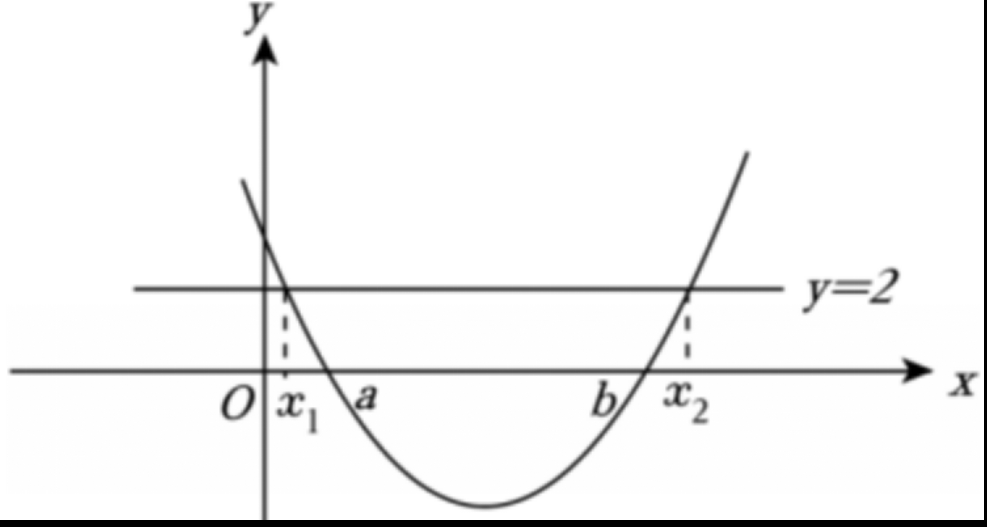
\includegraphics[width=0.42\textwidth]{figures/gao100_q16_parabola.png}
\end{center}
\step{所以数形结合得 $x_1<a<b<x_2$．故选 $B$.}
\solend
\fi

\end{enumerate}

\bigsec{三、解答题}

\begin{enumerate}
\setcounter{enumi}{16}

\item 已知集合 $A=\{x\mid3<x\leqslant6\}$，$B=\{x\mid m\leqslant x\leqslant2m+1\}$.

（1）若 $m=2$，求 $A\cap B$、$A\cup B$；

（2）若 $x\in B$ 是 $x\in A$ 的必要条件，求实数 $m$ 的取值范围.

\ansspace*[9]

\ifanswer
\solbegin
\stepm{（1）}{若 $m=2$，则 $B=\{x\mid2\leqslant x\leqslant5\}$，因为 $A=\{x\mid3<x\leqslant6\}$，}
\step{所以 $A\cap B=\{x\mid3<x\leqslant5\}$，$A\cup B=\{x\mid2\leqslant x\leqslant6\}$.}
\stepm{（2）}{因为 $x\in B$ 是 $x\in A$ 的必要条件，所以 $A\subseteq B$，}
\step{所以 $\begin{cases}m\leqslant3\\ 2m+1\geqslant6\end{cases}$，所以 $\dfrac52\leqslant m\leqslant3$，所以实数 $m$ 的取值范围为 $\left[\dfrac52,3\right]$.}
\solend
\fi

\item 求关于 $x$ 的不等式 $3ax^2-(3a+2)x+2<0\,(a\in R)$ 的解集.

\ansspace*[10]

\ifanswer
\solbegin
\step{当 $a=0$ 时，不等式化为 $-2x+2<0$，解得 $x>1$，}
\step{当 $a\neq0$ 时，方程 $3ax^2-(3a+2)x+2=0$ 的两根分别为 $1$，$\dfrac2{3a}$}
\step{当 $\dfrac2{3a}=1$，即 $a=\dfrac23$ 时，不等式化为 $(x-1)^2<0$，不等式无解，}
\step{当 $\dfrac2{3a}<1$，即 $a>\dfrac23$ 时，不等式解集为 $\left(\dfrac2{3a},1\right)$，}
\step{当 $0<a<\dfrac23$ 时，$\dfrac2{3a}>1$，不等式的解集为 $\left(1,\dfrac2{3a}\right)$，}
\step{当 $a<0$ 时，不等式的解集为 $\left(-\infty,\dfrac2{3a}\right)\cup(1,+\infty)$，}
\step{综上，当 $a=0$ 时，不等式的解集为 $(1,+\infty)$，}
\step{当 $a=\dfrac23$ 时，不等式的解集为 $\varnothing$，}
\step{当 $a>\dfrac23$ 时，不等式解集为 $\left(\dfrac2{3a},1\right)$，}
\step{当 $0<a<\dfrac23$ 时，不等式的解集为 $\left(1,\dfrac2{3a}\right)$，}
\step{当 $a<0$ 时，不等式的解集为 $\left(-\infty,\dfrac2{3a}\right)\cup(1,+\infty)$.}
\solend
\fi

\item 设对于任意实数 $x$，不等式 $\lvert x+1\rvert+\lvert x-1\rvert\geqslant m$ 恒成立.

（1）求 $m$ 的取值范围；

（2）当 $m$ 取最大值时，解关于 $x$ 的不等式 $\lvert x-3\rvert-2x\leqslant2m-2$.

\ansspace*[9]

\ifanswer
\solbegin
\stepm{（1）}{设函数 $f(x)=\lvert x+1\rvert+\lvert x-1\rvert$，则 $f(x)=\begin{cases}-2x,&x\leqslant-1\\ 2,&-1<x<1\\ 2x,&x\geqslant1\end{cases}$，}
\step{当 $x\leqslant-1$ 时，$f(x)$ 有最小值 2；}
\step{当 $-1<x<1$ 时，$f(x)=2$；}
\step{当 $x\geqslant1$ 时，$f(x)$ 有最小值 2；}
\step{因为对于任意实数 $x$，不等式 $\lvert x+1\rvert+\lvert x-1\rvert\geqslant m$ 恒成立，}
\step{所以 $m\leqslant2$，即 $m$ 的取值范围为 $(-\infty,2]$；}
\stepm{（2）}{由（1）得 $m$ 的最大值为 2，所以原不等式为 $\lvert x-3\rvert\leqslant2x+2$，}
\step{即 $-2x-2\leqslant x-3\leqslant2x+2$，解得 $x\geqslant\dfrac13$，}
\step{所以原不等式的解集为 $\left\{x\mid x\geqslant\dfrac13\right\}$.}
\solend
\fi

\item 某轮船公司的一艘轮船每小时花费的燃料费与轮船航行速度的平方成正比，比例系数为 $k$．轮船的最大速度为 18 海里/小时．当船速为 10 海里/小时，它的燃料费是每小时 120 元，其余航行运作费用（不论速度如何）总计是每小时 120 元．假定运行过程中轮船以速度 $v$ 匀速航行.

（1）求 $k$ 的值及每小时的最大总费用 $H$；

（2）求该轮船航行 100 海里的总费用 $W$（燃料费＋其余航行运作费用）的最小值.

\ansspace*[10]

\ifanswer
\solbegin
\stepm{（1）}{由题意，每小时燃料费为 $h(v)=kv^2$，$0<v\leqslant18$，}
\step{已知 $v=10$ 时，燃料费每小时 120 元，则 $k\cdot10^2=120$，得 $k=1.2$，}
\step{每小时总费用 $h(v)=kv^2+120=1.2v^2+120$，}
\step{$h(v)$ 是关于 $v$ 的增函数，$v$ 最大为 18，}
\step{所以 $H=h(18)=1.2\times18^2+120=508.8$ 元.}
\stepm{（2）}{航行时间 $t=\dfrac{100}v$ 小时，}
\step{$W(v)=h(v)\cdot t=(1.2v^2+120)\cdot\dfrac{100}v,0<v\leqslant18=120v+\dfrac{12000}v$，}
\step{利用均值不等式 $120v+\dfrac{12000}v\geqslant2\sqrt{120v\cdot\dfrac{12000}v}=2\times1200=2400$，}
\step{当且仅当 $120v=\dfrac{12000}v$，即 $v=10$ 时取等号，}
\step{$v=10\leqslant18$，在速度范围内，可取到等号，所以总费用最小值为 2400 元.}
\solend
\fi

\item 已知 $A$ 是 $R$ 的非空真子集，如果对任意 $x$、$y\in A$，都有 $x+y\in A$，$xy\in A$，则称 $A$ 是封闭集.

（1）判断集合 $B=\{0\}$，$C=\{-1,0,1\}$ 是否为封闭集，并说明理由；

（2）判断以下两个命题的真假，并说明理由；

命题 $p$：若非空集合 $A_1$、$A_2$ 是封闭集，则 $A_1\cup A_2$ 也是封闭集；

命题 $q$：非空集合 $A_1$、$A_2$ 是封闭集，则 $A_1\cap A_2\neq\varnothing$ 是 $A_1\cap A_2$ 是封闭集的充要条件；

（3）若非空集合 $A$ 是封闭集合，设全集为 $R$，求证：$A$ 的补集不是封闭集.

\ansspace*[13]

\ifanswer
\solbegin
\stepm{（1）}{$B=\{0\}$ 是封闭集，$C=\{-1,0,1\}$ 不是封闭集，理由如下：}
\step{对于集合 $B=\{0\}$，因为 $0+0=0\in B$，$0\times0=0\in B$，}
\step{所以 $B=\{0\}$ 是封闭集；}
\step{对于集合 $C=\{-1,0,1\}$，因为 $-1+(-1)=-2\notin C$，$1+1=2\notin C$，}
\step{所以集合 $C=\{-1,0,1\}$ 不是封闭集.}
\stepm{（2）}{命题 $p$ 是假命题，命题 $q$ 是真命题，理由如下：}
\step{对命题 $p$：令 $A_1=\{x\mid x=2k,k\in Z\}$，$A_2=\{x\mid x=3k,k\in Z\}$，}
\step{令 $x_1=2k_1$，$y_1=2k_2$，$k_1$、$k_2\in Z$，}
\step{则 $x_1+y_1=2(k_1+k_2)\in A_1$，$x_1y_1=2(2k_1k_2)\in A_1$，}
\step{因此集合 $A_1$ 是封闭集，同理集合 $A_2$ 也是封闭集，}
\step{取 $x_2=2$，$y_2=3$，则 $x_2$、$y_2\in(A_1\cup A_2)$，而 $x_2+y_2=5\notin(A_1\cup A_2)$，}
\step{因此集合 $A_1\cup A_2$ 不是封闭集，命题 $p$ 是假命题；}
\step{对于命题 $q$：若 $A_1\cap A_2\neq\varnothing$，不妨令 $a$、$b\in(A_1\cap A_2)$，}
\step{则有 $a$、$b\in A_1$，又集合 $A_1$ 是封闭集，则 $a+b\in A_1$，$ab\in A_1$，}
\step{同理 $a+b\in A_2$，$ab\in A_2$，因此 $a+b\in(A_1\cap A_2)$，$ab\in(A_1\cap A_2)$，}
\step{所以 $A_1\cap A_2$ 是封闭集；}
\step{反之，若 $A_1\cap A_2$ 是封闭集，则 $A_1\cap A_2$ 是非空集合，即 $A_1\cap A_2\neq\varnothing$，}
\step{所以 $A_1\cap A_2$ 是 $A_1\cap A_2$ 是封闭集的充要条件，命题 $q$ 是真命题.}
\stepm{（3）}{非空集合 $A$ 是封闭集合，当 $A=R$ 时，$\overline A=\varnothing$，因此 $\overline A$ 不是封闭集合；}
\step{当 $A\neq R$ 时，假设 $\overline A$ 是封闭集合，}
\step{设 $0\in A$，在 $\overline A$ 中任取一个 $x$，$x\neq0$，则 $-x\in A$，}
\step{否则 $-x\in\overline A$，此时 $x+(-x)=0\in\overline A$，与 $0\in A$ 矛盾，}
\step{因此 $(-x)^2\in A$，$x^2\in\overline A$，而 $(-x)^2=x^2$，与 $A\cap\overline A=\varnothing$ 矛盾，}
\step{则当 $0\in A$ 时，则 $\overline A$ 不是封闭集合，同理当 $0\in\overline A$ 时，$\overline A$ 不是封闭集合，}
\step{所以 $A$ 的补集不是封闭集.}
\solend
\fi

\end{enumerate}

\end{document}
"
%
% 原始材料：微信公众号“魔都数学加油站”文章，连载“27学年高一100”；
% 原文标题“27学年高一100——2026-2027年上海市南洋中学高一上10月月考”；
% 原文链接：https://mp.weixin.qq.com/s/uXLyt6VHraW4hSpDwnZDuQ。
% 正文为 10 张 PNG 页（`原图/高一100_南洋中学_10月月考/01..10.png`），
% 尺寸混排（第 2、4—9 页为 4762×6735，第 1、3、10 页为 2560×3620），按页序读取。
%
% 篇幅与题号：原卷自第 3 题起编号（第 1、2 题不在原文内）。填空题 3—12（10 题）、
% 选择题 13—16（4 题）、解答题 17—21（5 题），共 19 题。
%
% 讲评版：全部 19 题均印【解析】，其中第 13—16 题的答案在解析末句
% “故选 $C$／$B$／$D$／$B$”（题干括号内未印答案）。第 16 题解析带一幅
% 抛物线与 $y=2$ 的示意图，自原图裁切、去粉色水印后转灰度，三版都出。
%
% 副标题：原卷未印副标题。本稿按内容标作“集合与常用逻辑用语、不等式”。
%
% 原卷笔误/存疑（均照录未改，正文对应处另有 % 注）：无。
%
% 与原卷的排版差异：
%   ① 原卷每题下直接印【解析】，本稿按全稿惯例将答案与解析置于答案版；
%   ② 原卷未印副标题，本稿补出；填空横线统一排 \blankline[4.4em]；
%   ③ 原卷数集记号排斜体 $R$、$Z$、$\mathit N$，本稿按全稿惯例改用 $\R$、$\Z$、$\N$；
%   ④ 解答题按惯例加 \ansspace；选择题括号排 \mbox{（\quad）}；
%   ⑤ 第 16 题的示意图原卷排在解析行右侧，本稿改排为解析后的居中图。
%
% 行数核对：逐题数 \step/\stepm 条数，合计 117 条（Q3：2；Q4：5；Q5：7；Q6：3；Q7：3；
% Q8：4；Q9：2；Q10：4；Q11：6；Q12：3；Q13：7；Q14：3；Q15：5；Q16：3；Q17：5；
% Q18：11；Q19：9；Q20：10；Q21：25）。全卷 19 题均印【解析】。
% 原卷解析的换行按语意合并，未逐行强拆。
%
\documentclass[a4paper,11pt]{article}
\usepackage{common}
\begin{document}

\examtitlest[7]{2026--2027 年南洋中学高一上 10 月月考}{集合与常用逻辑用语、不等式}

\bigsec{一、填空题}

\begin{enumerate}
\setcounter{enumi}{2}

\item 不等式 $\dfrac{x-6}{x+1}\geqslant0$ 的解集为\blankline[4.4em].

\ifanswer
\solbegin
\step{不等式 $\dfrac{x-6}{x+1}\geqslant0$ 等价于 $\begin{cases}(x-6)(x+1)\geqslant0\\ x+1\neq0\end{cases}$，即 $x<-1$ 或 $x\geqslant6$，}
\step{故解集为 $(-\infty,-1)\cup[6,+\infty)$.}
\solend
\fi

\item 已知关于 $x$ 的不等式 $ax^2+bx+c>0$ 的解集是 $(1,3)$，则关于 $x$ 的不等式 $ax^2-bx+c\leqslant0$ 的解集为\blankline[4.4em].

\ifanswer
\solbegin
\step{由已知得 $a<0$，且 $1$，$3$ 是方程 $ax^2+bx+c=0$ 的根，}
\step{所以 $\begin{cases}1+3=-\dfrac ba\\[2pt] 1\times3=\dfrac ca\end{cases}$，所以 $\begin{cases}b=-4a\\ c=3a\end{cases}$，}
\step{所以 $ax^2-bx+c\leqslant0$ 可变形为 $ax^2+4ax+3a\leqslant0$，}
\step{因为 $a<0$，所以 $x^2+4x+3\geqslant0$，解得 $x\leqslant-3$ 或 $x\geqslant-1$，}
\step{所以不等式的解集为 $(-\infty,-3]\cup[-1,+\infty)$.}
\solend
\fi

\item 不等式 $\lvert x+2\rvert+\lvert 2x-1\rvert\geqslant3$ 的解集为\blankline[4.4em].

\ifanswer
\solbegin
\step{当 $x\leqslant-2$ 时，$x+2\leqslant0$，$2x-1<0$，}
\step{所以 $\lvert x+2\rvert+\lvert 2x-1\rvert=-x-2-2x+1\geqslant3$，解得 $x\leqslant-\dfrac43$；}
\step{当 $-2<x<\dfrac12$ 时，$x+2>0$，$2x-1<0$，}
\step{所以 $\lvert x+2\rvert+\lvert 2x-1\rvert=x+2-2x+1\geqslant3$，解得 $x\leqslant0$；}
\step{当 $x\geqslant\dfrac12$ 时，$x+2>0$，$2x-1\geqslant0$，}
\step{所以 $\lvert x+2\rvert+\lvert 2x-1\rvert=x+2+2x-1\geqslant3$，解得 $x\geqslant\dfrac23$；}
\step{所以原不等式的解集为 $\left\{x\mid x\leqslant0\right.$ 或 $\left.x\geqslant\dfrac23\right\}$.}
\solend
\fi

\item 若正数 $x$、$y$ 满足 $x+2y=2$，则 $\dfrac1x+\dfrac2y$ 的最小值是\blankline[4.4em].

\ifanswer
\solbegin
\step{因为 $x>0$，$y>0$，且 $x+2y=2$，}
\step{所以 $\dfrac1x+\dfrac2y=\dfrac12\left(\dfrac1x+\dfrac2y\right)(x+2y)=\dfrac12\left(5+\dfrac{2y}x+\dfrac{2x}y\right)\geqslant\dfrac12\left(5+2\sqrt{\dfrac{2y}x\cdot\dfrac{2x}y}\right)=\dfrac92$.}
\step{当且仅当 $\begin{cases}x+2y=2\\ \dfrac{2y}x=\dfrac{2x}y\end{cases}$，即 $x=y=\dfrac23$ 时取等号，故最小值为 $\dfrac92$.}
\solend
\fi

\item 已知 $\alpha:x\leqslant2$ 或 $x>3$，$\beta:x\leqslant m+5$ 或 $x>-m$，若 $\alpha$ 是 $\beta$ 的必要非充分条件，则实数 $m$ 的取值范围是\blankline[4.4em].

\ifanswer
\solbegin
\step{设 $A=\{x\mid x\leqslant2$ 或 $x>3\}$，$B=\{x\mid x\leqslant m+5$ 或 $x>-m\}$，则 $B\subset A$，}
\step{则 $m+5\leqslant2$ 且 $-m\geqslant3$（等号不能同时取得），则 $m<-3$，}
\step{则实数 $m$ 的取值范围是 $(-\infty,-3)$.}
\solend
\fi

\item 已知集合 $A=\{x\mid-1\leqslant x\leqslant3\}$，$B=\{x\mid ax+1>0\}$ 满足 $A\subseteq B$，则实数 $a$ 的取值范围为\blankline[4.4em].

\ifanswer
\solbegin
\step{当 $a=0$ 时，$B=R$，显然符合题意，}
\step{当 $a>0$ 时，$B=\left\{x\mid x>-\dfrac1a\right\}$，则 $-\dfrac1a<-1$，解得 $a<1$，所以 $0<a<1$，}
\step{当 $a<0$ 时，$B=\left\{x\mid x<-\dfrac1a\right\}$，则 $-\dfrac1a>3$，解得 $a>-\dfrac13$，所以 $-\dfrac13<a<0$，}
\step{综上所述，实数 $a$ 的取值范围为 $\left(-\dfrac13,1\right)$.}
\solend
\fi

\item 设集合 $A=\{x\mid3x-1<m\}$，若 $1\in A$ 且 $2\notin A$，则实数 $m$ 的取值范围是\blankline[4.4em].

\ifanswer
\solbegin
\step{因为集合 $A=\{x\mid3x-1<m\}$，若 $1\in A$ 且 $2\notin A$，}
\step{则 $3\times1-1<m$ 且 $3\times2-1\geqslant m$，解得 $2<m\leqslant5$.}
\solend
\fi

\item 若 $M=\left\{x\mid x=m+\dfrac16,m\in Z\right\},N=\left\{x\mid x=\dfrac n2-\dfrac13,n\in Z\right\}$，\newline $P=\left\{x\mid x=\dfrac p2+\dfrac16,p\in Z\right\}$，则 $M$、$N$、$P$ 的关系为\blankline[4.4em].

\ifanswer
\solbegin
\step{$M=\left\{x\mid x=m+\dfrac16=\dfrac{6m+1}6=\dfrac{3\cdot2m+1}6,m\in Z\right\}$，}
\step{$N=\left\{x\mid x=\dfrac n2-\dfrac13=\dfrac{3(n-1)+1}6,n\in Z\right\}=\left\{x\mid x=\dfrac{3k+1}6,k\in Z\right\}$，}
\step{$P=\left\{x\mid x=\dfrac p2+\dfrac16=\dfrac{3p+1}6,p\in Z\right\}$，}
\step{故 $M\subset N=P$.}
\solend
\fi

\item 已知命题 $p:x<-2$ 或 $x>3$，命题 $q:x<3m+1$ 或 $x>m+2$，若 $p$ 是 $q$ 的充分非必要条件，则实数 $m$ 的取值范围是\blankline[4.4em].

\ifanswer
\solbegin
\step{设 $A=\{x\mid x<-2$ 或 $x>3\}$，$B=\{x\mid x<3m+1$ 或 $x>m+2\}$，}
\step{若 $p$ 是 $q$ 的充分非必要条件，则 $A\subset B$，}
\step{当 $3m+1\geqslant m+2$，即 $m\geqslant\dfrac12$ 时，显然有 $A\subset B$，}
\step{当 $3m+1<m+2$，即 $m<\dfrac12$ 时，}
\step{由 $A\subset B$，则 $\begin{cases}m+2\leqslant3\\ 3m+1\geqslant-2\end{cases}$（等号不同时成立），即 $-1\leqslant m<\dfrac12$.}
\step{综上，实数 $m$ 的取值范围是 $[-1,+\infty)$.}
\solend
\fi

\item 对于一个有限集 $A$，一般都可以找到两个非空数集 $A_1$ 和 $A_2$，满足 $A_1\cap A_2=\varnothing$，且 $A_1\cup A_2=A$，记集合 $\{A_1,A_2\}$ 为 $A$ 的一个“划分集”．若 $A$ 中有 $n(n\geqslant2,n\in\N)$ 个元素，则不同的“划分集”共有\blankline[4.4em]个(用含 $n$ 的表达式填空).

\ifanswer
\solbegin
\step{集合中的每个元素都有属于 $A_1$ 或属于 $A_2$ 两种情况，故共有 $2^n$ 种情况，}
\step{排除全都属于 $A_1$ 或 $A_2$ 的两种情况，考虑对称情况，}
\step{故不同的“划分集”共有 $\dfrac12(2^n-2)=2^{n-1}-1$ 个.}
\solend
\fi

\end{enumerate}

\bigsec{二、选择题}

\begin{enumerate}
\setcounter{enumi}{12}

\item 下列命题中正确的\mbox{（\quad）}

\keepwithprev
A. $\varnothing$ 与 $\{0\}$ 表示同一个集合

B. 方程 $\{x\mid(x-2)^2(x-3)=0\}$ 的所有解的集合可表示为 $\{2,2,3\}$

C. 由 3，4，5 组成的集合可表示为 $\{3,4,5\}$ 或 $\{4,5,3\}$

D. 很小的实数可以构成集合.

\ifanswer
\solbegin
\step{对于 $A$，$\{0\}$ 中有一个元素 0，$\varnothing$ 中无任何元素，故 $\varnothing$ 与 $\{0\}$ 不是同一个集合，}
\step{故 $A$ 错误；}
\step{对于 $B$，$\{2,2,3\}$ 不满足集合元素的互异性，故 $B$ 错误；}
\step{对于 $C$，由集合的无序性，得由 3，4，5 组成的集合可表示为 $\{3,4,5\}$ 或 $\{4,5,3\}$，}
\step{故 $C$ 正确；}
\step{对于 $D$，由集合的确定性，很小的实数不能构成集合，故 $D$ 错误.}
\step{故选 $C$.}
\solend
\fi

\item 已知 $a\in R$，则“$\dfrac1a<1$”是“$a>1$”的\mbox{（\quad）}条件.

\keepwithprev
A. 充分非必要\qquad B. 必要非充分

C. 充要\qquad D. 既非充分又非必要

\ifanswer
\solbegin
\step{解 $\dfrac1a<1$，得 $a<0$ 或 $a>1$，}
\step{由 $a<0$ 或 $a>1$ 得不出 $a>1$，由 $a>1$ 得出 $a<0$ 或 $a>1$，}
\step{所以“$\dfrac1a<1$”是“$a>1$”的必要不充分条件．故选 $B$.}
\solend
\fi

\item 若命题“存在 $x_0\in R$ 使得 $ax_0^2+2ax_0+1\leqslant0$”是假命题，则实数 $a$ 的取值范围为\mbox{（\quad）}

\keepwithprev
A. $a<0$ 或 $a\geqslant1$\qquad B. $a\leqslant0$ 或 $a\geqslant1$\qquad C. $0<a<1$\qquad D. $0\leqslant a<1$

\ifanswer
\solbegin
\step{命题“存在 $x_0\in R$ 使得 $ax_0^2+2ax_0+1\leqslant0$”是假命题，}
\step{则 $\forall x\in R$，$ax^2+2ax+1>0$ 恒成立，}
\step{当 $a=0$ 时，满足题意，}
\step{当 $a\neq0$ 时，$\begin{cases}a>0\\ \Delta=4a^2-4a<0\end{cases}$，解得 $0<a<1$，}
\step{综上所述，实数 $a$ 的取值范围为 $\{a\mid0\leqslant a<1\}$．故选 $D$.}
\solend
\fi

\item 已知实数 $a<b$，关于 $x$ 的不等式 $x^2-(a+b)x+ab-2<0$ 的解集为 $(x_1,x_2)$，则实数 $a$、$b$、$x_1$、$x_2$ 从小到大的排列是\mbox{（\quad）}

\keepwithprev
A. $a<x_1<x_2<b$\qquad B. $x_1<a<b<x_2$\qquad C. $a<x_1<b<x_2$\qquad D. $x_1<a<x_2<b$

\ifanswer
\solbegin
\step{因为实数 $a<b$，不等式 $x^2-(a+b)x+ab-2<0$ 可化为 $(x-a)(x-b)<2$，}
\step{又其解集为 $(x_1,x_2)$，所以作出 $y=(x-a)(x-b)$ 与 $y=2$ 的图象如下：}
\begin{center}
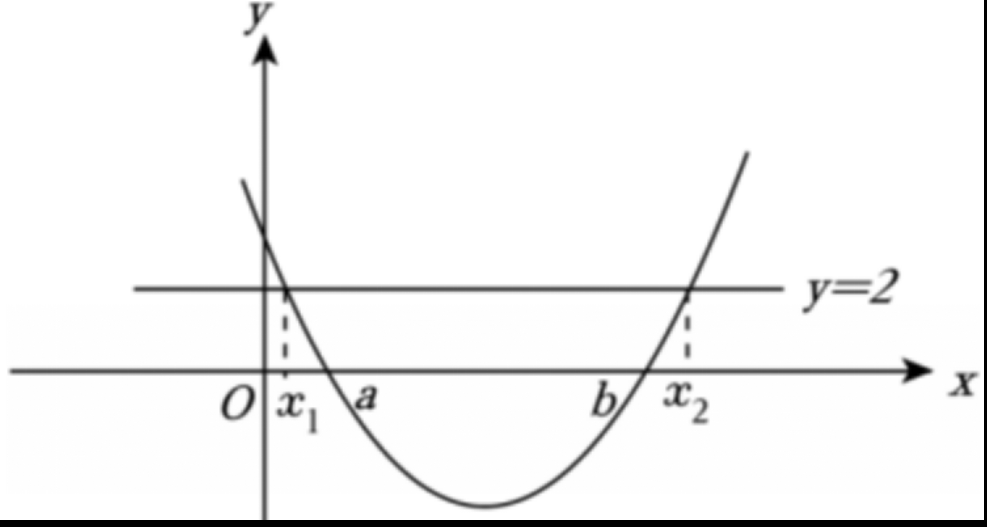
\includegraphics[width=0.42\textwidth]{figures/gao100_q16_parabola.png}
\end{center}
\step{所以数形结合得 $x_1<a<b<x_2$．故选 $B$.}
\solend
\fi

\end{enumerate}

\bigsec{三、解答题}

\begin{enumerate}
\setcounter{enumi}{16}

\item 已知集合 $A=\{x\mid3<x\leqslant6\}$，$B=\{x\mid m\leqslant x\leqslant2m+1\}$.

（1）若 $m=2$，求 $A\cap B$、$A\cup B$；

（2）若 $x\in B$ 是 $x\in A$ 的必要条件，求实数 $m$ 的取值范围.

\ansspace*[9]

\ifanswer
\solbegin
\stepm{（1）}{若 $m=2$，则 $B=\{x\mid2\leqslant x\leqslant5\}$，因为 $A=\{x\mid3<x\leqslant6\}$，}
\step{所以 $A\cap B=\{x\mid3<x\leqslant5\}$，$A\cup B=\{x\mid2\leqslant x\leqslant6\}$.}
\stepm{（2）}{因为 $x\in B$ 是 $x\in A$ 的必要条件，所以 $A\subseteq B$，}
\step{所以 $\begin{cases}m\leqslant3\\ 2m+1\geqslant6\end{cases}$，所以 $\dfrac52\leqslant m\leqslant3$，所以实数 $m$ 的取值范围为 $\left[\dfrac52,3\right]$.}
\solend
\fi

\item 求关于 $x$ 的不等式 $3ax^2-(3a+2)x+2<0\,(a\in R)$ 的解集.

\ansspace*[10]

\ifanswer
\solbegin
\step{当 $a=0$ 时，不等式化为 $-2x+2<0$，解得 $x>1$，}
\step{当 $a\neq0$ 时，方程 $3ax^2-(3a+2)x+2=0$ 的两根分别为 $1$，$\dfrac2{3a}$}
\step{当 $\dfrac2{3a}=1$，即 $a=\dfrac23$ 时，不等式化为 $(x-1)^2<0$，不等式无解，}
\step{当 $\dfrac2{3a}<1$，即 $a>\dfrac23$ 时，不等式解集为 $\left(\dfrac2{3a},1\right)$，}
\step{当 $0<a<\dfrac23$ 时，$\dfrac2{3a}>1$，不等式的解集为 $\left(1,\dfrac2{3a}\right)$，}
\step{当 $a<0$ 时，不等式的解集为 $\left(-\infty,\dfrac2{3a}\right)\cup(1,+\infty)$，}
\step{综上，当 $a=0$ 时，不等式的解集为 $(1,+\infty)$，}
\step{当 $a=\dfrac23$ 时，不等式的解集为 $\varnothing$，}
\step{当 $a>\dfrac23$ 时，不等式解集为 $\left(\dfrac2{3a},1\right)$，}
\step{当 $0<a<\dfrac23$ 时，不等式的解集为 $\left(1,\dfrac2{3a}\right)$，}
\step{当 $a<0$ 时，不等式的解集为 $\left(-\infty,\dfrac2{3a}\right)\cup(1,+\infty)$.}
\solend
\fi

\item 设对于任意实数 $x$，不等式 $\lvert x+1\rvert+\lvert x-1\rvert\geqslant m$ 恒成立.

（1）求 $m$ 的取值范围；

（2）当 $m$ 取最大值时，解关于 $x$ 的不等式 $\lvert x-3\rvert-2x\leqslant2m-2$.

\ansspace*[9]

\ifanswer
\solbegin
\stepm{（1）}{设函数 $f(x)=\lvert x+1\rvert+\lvert x-1\rvert$，则 $f(x)=\begin{cases}-2x,&x\leqslant-1\\ 2,&-1<x<1\\ 2x,&x\geqslant1\end{cases}$，}
\step{当 $x\leqslant-1$ 时，$f(x)$ 有最小值 2；}
\step{当 $-1<x<1$ 时，$f(x)=2$；}
\step{当 $x\geqslant1$ 时，$f(x)$ 有最小值 2；}
\step{因为对于任意实数 $x$，不等式 $\lvert x+1\rvert+\lvert x-1\rvert\geqslant m$ 恒成立，}
\step{所以 $m\leqslant2$，即 $m$ 的取值范围为 $(-\infty,2]$；}
\stepm{（2）}{由（1）得 $m$ 的最大值为 2，所以原不等式为 $\lvert x-3\rvert\leqslant2x+2$，}
\step{即 $-2x-2\leqslant x-3\leqslant2x+2$，解得 $x\geqslant\dfrac13$，}
\step{所以原不等式的解集为 $\left\{x\mid x\geqslant\dfrac13\right\}$.}
\solend
\fi

\item 某轮船公司的一艘轮船每小时花费的燃料费与轮船航行速度的平方成正比，比例系数为 $k$．轮船的最大速度为 18 海里/小时．当船速为 10 海里/小时，它的燃料费是每小时 120 元，其余航行运作费用（不论速度如何）总计是每小时 120 元．假定运行过程中轮船以速度 $v$ 匀速航行.

（1）求 $k$ 的值及每小时的最大总费用 $H$；

（2）求该轮船航行 100 海里的总费用 $W$（燃料费＋其余航行运作费用）的最小值.

\ansspace*[10]

\ifanswer
\solbegin
\stepm{（1）}{由题意，每小时燃料费为 $h(v)=kv^2$，$0<v\leqslant18$，}
\step{已知 $v=10$ 时，燃料费每小时 120 元，则 $k\cdot10^2=120$，得 $k=1.2$，}
\step{每小时总费用 $h(v)=kv^2+120=1.2v^2+120$，}
\step{$h(v)$ 是关于 $v$ 的增函数，$v$ 最大为 18，}
\step{所以 $H=h(18)=1.2\times18^2+120=508.8$ 元.}
\stepm{（2）}{航行时间 $t=\dfrac{100}v$ 小时，}
\step{$W(v)=h(v)\cdot t=(1.2v^2+120)\cdot\dfrac{100}v,0<v\leqslant18=120v+\dfrac{12000}v$，}
\step{利用均值不等式 $120v+\dfrac{12000}v\geqslant2\sqrt{120v\cdot\dfrac{12000}v}=2\times1200=2400$，}
\step{当且仅当 $120v=\dfrac{12000}v$，即 $v=10$ 时取等号，}
\step{$v=10\leqslant18$，在速度范围内，可取到等号，所以总费用最小值为 2400 元.}
\solend
\fi

\item 已知 $A$ 是 $R$ 的非空真子集，如果对任意 $x$、$y\in A$，都有 $x+y\in A$，$xy\in A$，则称 $A$ 是封闭集.

（1）判断集合 $B=\{0\}$，$C=\{-1,0,1\}$ 是否为封闭集，并说明理由；

（2）判断以下两个命题的真假，并说明理由；

命题 $p$：若非空集合 $A_1$、$A_2$ 是封闭集，则 $A_1\cup A_2$ 也是封闭集；

命题 $q$：非空集合 $A_1$、$A_2$ 是封闭集，则 $A_1\cap A_2\neq\varnothing$ 是 $A_1\cap A_2$ 是封闭集的充要条件；

（3）若非空集合 $A$ 是封闭集合，设全集为 $R$，求证：$A$ 的补集不是封闭集.

\ansspace*[13]

\ifanswer
\solbegin
\stepm{（1）}{$B=\{0\}$ 是封闭集，$C=\{-1,0,1\}$ 不是封闭集，理由如下：}
\step{对于集合 $B=\{0\}$，因为 $0+0=0\in B$，$0\times0=0\in B$，}
\step{所以 $B=\{0\}$ 是封闭集；}
\step{对于集合 $C=\{-1,0,1\}$，因为 $-1+(-1)=-2\notin C$，$1+1=2\notin C$，}
\step{所以集合 $C=\{-1,0,1\}$ 不是封闭集.}
\stepm{（2）}{命题 $p$ 是假命题，命题 $q$ 是真命题，理由如下：}
\step{对命题 $p$：令 $A_1=\{x\mid x=2k,k\in Z\}$，$A_2=\{x\mid x=3k,k\in Z\}$，}
\step{令 $x_1=2k_1$，$y_1=2k_2$，$k_1$、$k_2\in Z$，}
\step{则 $x_1+y_1=2(k_1+k_2)\in A_1$，$x_1y_1=2(2k_1k_2)\in A_1$，}
\step{因此集合 $A_1$ 是封闭集，同理集合 $A_2$ 也是封闭集，}
\step{取 $x_2=2$，$y_2=3$，则 $x_2$、$y_2\in(A_1\cup A_2)$，而 $x_2+y_2=5\notin(A_1\cup A_2)$，}
\step{因此集合 $A_1\cup A_2$ 不是封闭集，命题 $p$ 是假命题；}
\step{对于命题 $q$：若 $A_1\cap A_2\neq\varnothing$，不妨令 $a$、$b\in(A_1\cap A_2)$，}
\step{则有 $a$、$b\in A_1$，又集合 $A_1$ 是封闭集，则 $a+b\in A_1$，$ab\in A_1$，}
\step{同理 $a+b\in A_2$，$ab\in A_2$，因此 $a+b\in(A_1\cap A_2)$，$ab\in(A_1\cap A_2)$，}
\step{所以 $A_1\cap A_2$ 是封闭集；}
\step{反之，若 $A_1\cap A_2$ 是封闭集，则 $A_1\cap A_2$ 是非空集合，即 $A_1\cap A_2\neq\varnothing$，}
\step{所以 $A_1\cap A_2$ 是 $A_1\cap A_2$ 是封闭集的充要条件，命题 $q$ 是真命题.}
\stepm{（3）}{非空集合 $A$ 是封闭集合，当 $A=R$ 时，$\overline A=\varnothing$，因此 $\overline A$ 不是封闭集合；}
\step{当 $A\neq R$ 时，假设 $\overline A$ 是封闭集合，}
\step{设 $0\in A$，在 $\overline A$ 中任取一个 $x$，$x\neq0$，则 $-x\in A$，}
\step{否则 $-x\in\overline A$，此时 $x+(-x)=0\in\overline A$，与 $0\in A$ 矛盾，}
\step{因此 $(-x)^2\in A$，$x^2\in\overline A$，而 $(-x)^2=x^2$，与 $A\cap\overline A=\varnothing$ 矛盾，}
\step{则当 $0\in A$ 时，则 $\overline A$ 不是封闭集合，同理当 $0\in\overline A$ 时，$\overline A$ 不是封闭集合，}
\step{所以 $A$ 的补集不是封闭集.}
\solend
\fi

\end{enumerate}

\end{document}
"
% 紧凑版：xelatex "\def\iscompact{1}% 高一100_南洋中学_10月月考.tex
%   —— 高一上数学“2026-2027 年南洋中学高一上 10 月月考”（讲评版）
% 试卷版：xelatex 高一100_南洋中学_10月月考.tex
% 答案版：xelatex "\def\isanswer{1}% 高一100_南洋中学_10月月考.tex
%   —— 高一上数学“2026-2027 年南洋中学高一上 10 月月考”（讲评版）
% 试卷版：xelatex 高一100_南洋中学_10月月考.tex
% 答案版：xelatex "\def\isanswer{1}% 高一100_南洋中学_10月月考.tex
%   —— 高一上数学“2026-2027 年南洋中学高一上 10 月月考”（讲评版）
% 试卷版：xelatex 高一100_南洋中学_10月月考.tex
% 答案版：xelatex "\def\isanswer{1}\input{高一100_南洋中学_10月月考.tex}"
% 紧凑版：xelatex "\def\iscompact{1}\input{高一100_南洋中学_10月月考.tex}"
%
% 原始材料：微信公众号“魔都数学加油站”文章，连载“27学年高一100”；
% 原文标题“27学年高一100——2026-2027年上海市南洋中学高一上10月月考”；
% 原文链接：https://mp.weixin.qq.com/s/uXLyt6VHraW4hSpDwnZDuQ。
% 正文为 10 张 PNG 页（`原图/高一100_南洋中学_10月月考/01..10.png`），
% 尺寸混排（第 2、4—9 页为 4762×6735，第 1、3、10 页为 2560×3620），按页序读取。
%
% 篇幅与题号：原卷自第 3 题起编号（第 1、2 题不在原文内）。填空题 3—12（10 题）、
% 选择题 13—16（4 题）、解答题 17—21（5 题），共 19 题。
%
% 讲评版：全部 19 题均印【解析】，其中第 13—16 题的答案在解析末句
% “故选 $C$／$B$／$D$／$B$”（题干括号内未印答案）。第 16 题解析带一幅
% 抛物线与 $y=2$ 的示意图，自原图裁切、去粉色水印后转灰度，三版都出。
%
% 副标题：原卷未印副标题。本稿按内容标作“集合与常用逻辑用语、不等式”。
%
% 原卷笔误/存疑（均照录未改，正文对应处另有 % 注）：无。
%
% 与原卷的排版差异：
%   ① 原卷每题下直接印【解析】，本稿按全稿惯例将答案与解析置于答案版；
%   ② 原卷未印副标题，本稿补出；填空横线统一排 \blankline[4.4em]；
%   ③ 原卷数集记号排斜体 $R$、$Z$、$\mathit N$，本稿按全稿惯例改用 $\R$、$\Z$、$\N$；
%   ④ 解答题按惯例加 \ansspace；选择题括号排 \mbox{（\quad）}；
%   ⑤ 第 16 题的示意图原卷排在解析行右侧，本稿改排为解析后的居中图。
%
% 行数核对：逐题数 \step/\stepm 条数，合计 117 条（Q3：2；Q4：5；Q5：7；Q6：3；Q7：3；
% Q8：4；Q9：2；Q10：4；Q11：6；Q12：3；Q13：7；Q14：3；Q15：5；Q16：3；Q17：5；
% Q18：11；Q19：9；Q20：10；Q21：25）。全卷 19 题均印【解析】。
% 原卷解析的换行按语意合并，未逐行强拆。
%
\documentclass[a4paper,11pt]{article}
\usepackage{common}
\begin{document}

\examtitlest[7]{2026--2027 年南洋中学高一上 10 月月考}{集合与常用逻辑用语、不等式}

\bigsec{一、填空题}

\begin{enumerate}
\setcounter{enumi}{2}

\item 不等式 $\dfrac{x-6}{x+1}\geqslant0$ 的解集为\blankline[4.4em].

\ifanswer
\solbegin
\step{不等式 $\dfrac{x-6}{x+1}\geqslant0$ 等价于 $\begin{cases}(x-6)(x+1)\geqslant0\\ x+1\neq0\end{cases}$，即 $x<-1$ 或 $x\geqslant6$，}
\step{故解集为 $(-\infty,-1)\cup[6,+\infty)$.}
\solend
\fi

\item 已知关于 $x$ 的不等式 $ax^2+bx+c>0$ 的解集是 $(1,3)$，则关于 $x$ 的不等式 $ax^2-bx+c\leqslant0$ 的解集为\blankline[4.4em].

\ifanswer
\solbegin
\step{由已知得 $a<0$，且 $1$，$3$ 是方程 $ax^2+bx+c=0$ 的根，}
\step{所以 $\begin{cases}1+3=-\dfrac ba\\[2pt] 1\times3=\dfrac ca\end{cases}$，所以 $\begin{cases}b=-4a\\ c=3a\end{cases}$，}
\step{所以 $ax^2-bx+c\leqslant0$ 可变形为 $ax^2+4ax+3a\leqslant0$，}
\step{因为 $a<0$，所以 $x^2+4x+3\geqslant0$，解得 $x\leqslant-3$ 或 $x\geqslant-1$，}
\step{所以不等式的解集为 $(-\infty,-3]\cup[-1,+\infty)$.}
\solend
\fi

\item 不等式 $\lvert x+2\rvert+\lvert 2x-1\rvert\geqslant3$ 的解集为\blankline[4.4em].

\ifanswer
\solbegin
\step{当 $x\leqslant-2$ 时，$x+2\leqslant0$，$2x-1<0$，}
\step{所以 $\lvert x+2\rvert+\lvert 2x-1\rvert=-x-2-2x+1\geqslant3$，解得 $x\leqslant-\dfrac43$；}
\step{当 $-2<x<\dfrac12$ 时，$x+2>0$，$2x-1<0$，}
\step{所以 $\lvert x+2\rvert+\lvert 2x-1\rvert=x+2-2x+1\geqslant3$，解得 $x\leqslant0$；}
\step{当 $x\geqslant\dfrac12$ 时，$x+2>0$，$2x-1\geqslant0$，}
\step{所以 $\lvert x+2\rvert+\lvert 2x-1\rvert=x+2+2x-1\geqslant3$，解得 $x\geqslant\dfrac23$；}
\step{所以原不等式的解集为 $\left\{x\mid x\leqslant0\right.$ 或 $\left.x\geqslant\dfrac23\right\}$.}
\solend
\fi

\item 若正数 $x$、$y$ 满足 $x+2y=2$，则 $\dfrac1x+\dfrac2y$ 的最小值是\blankline[4.4em].

\ifanswer
\solbegin
\step{因为 $x>0$，$y>0$，且 $x+2y=2$，}
\step{所以 $\dfrac1x+\dfrac2y=\dfrac12\left(\dfrac1x+\dfrac2y\right)(x+2y)=\dfrac12\left(5+\dfrac{2y}x+\dfrac{2x}y\right)\geqslant\dfrac12\left(5+2\sqrt{\dfrac{2y}x\cdot\dfrac{2x}y}\right)=\dfrac92$.}
\step{当且仅当 $\begin{cases}x+2y=2\\ \dfrac{2y}x=\dfrac{2x}y\end{cases}$，即 $x=y=\dfrac23$ 时取等号，故最小值为 $\dfrac92$.}
\solend
\fi

\item 已知 $\alpha:x\leqslant2$ 或 $x>3$，$\beta:x\leqslant m+5$ 或 $x>-m$，若 $\alpha$ 是 $\beta$ 的必要非充分条件，则实数 $m$ 的取值范围是\blankline[4.4em].

\ifanswer
\solbegin
\step{设 $A=\{x\mid x\leqslant2$ 或 $x>3\}$，$B=\{x\mid x\leqslant m+5$ 或 $x>-m\}$，则 $B\subset A$，}
\step{则 $m+5\leqslant2$ 且 $-m\geqslant3$（等号不能同时取得），则 $m<-3$，}
\step{则实数 $m$ 的取值范围是 $(-\infty,-3)$.}
\solend
\fi

\item 已知集合 $A=\{x\mid-1\leqslant x\leqslant3\}$，$B=\{x\mid ax+1>0\}$ 满足 $A\subseteq B$，则实数 $a$ 的取值范围为\blankline[4.4em].

\ifanswer
\solbegin
\step{当 $a=0$ 时，$B=R$，显然符合题意，}
\step{当 $a>0$ 时，$B=\left\{x\mid x>-\dfrac1a\right\}$，则 $-\dfrac1a<-1$，解得 $a<1$，所以 $0<a<1$，}
\step{当 $a<0$ 时，$B=\left\{x\mid x<-\dfrac1a\right\}$，则 $-\dfrac1a>3$，解得 $a>-\dfrac13$，所以 $-\dfrac13<a<0$，}
\step{综上所述，实数 $a$ 的取值范围为 $\left(-\dfrac13,1\right)$.}
\solend
\fi

\item 设集合 $A=\{x\mid3x-1<m\}$，若 $1\in A$ 且 $2\notin A$，则实数 $m$ 的取值范围是\blankline[4.4em].

\ifanswer
\solbegin
\step{因为集合 $A=\{x\mid3x-1<m\}$，若 $1\in A$ 且 $2\notin A$，}
\step{则 $3\times1-1<m$ 且 $3\times2-1\geqslant m$，解得 $2<m\leqslant5$.}
\solend
\fi

\item 若 $M=\left\{x\mid x=m+\dfrac16,m\in Z\right\},N=\left\{x\mid x=\dfrac n2-\dfrac13,n\in Z\right\}$，\newline $P=\left\{x\mid x=\dfrac p2+\dfrac16,p\in Z\right\}$，则 $M$、$N$、$P$ 的关系为\blankline[4.4em].

\ifanswer
\solbegin
\step{$M=\left\{x\mid x=m+\dfrac16=\dfrac{6m+1}6=\dfrac{3\cdot2m+1}6,m\in Z\right\}$，}
\step{$N=\left\{x\mid x=\dfrac n2-\dfrac13=\dfrac{3(n-1)+1}6,n\in Z\right\}=\left\{x\mid x=\dfrac{3k+1}6,k\in Z\right\}$，}
\step{$P=\left\{x\mid x=\dfrac p2+\dfrac16=\dfrac{3p+1}6,p\in Z\right\}$，}
\step{故 $M\subset N=P$.}
\solend
\fi

\item 已知命题 $p:x<-2$ 或 $x>3$，命题 $q:x<3m+1$ 或 $x>m+2$，若 $p$ 是 $q$ 的充分非必要条件，则实数 $m$ 的取值范围是\blankline[4.4em].

\ifanswer
\solbegin
\step{设 $A=\{x\mid x<-2$ 或 $x>3\}$，$B=\{x\mid x<3m+1$ 或 $x>m+2\}$，}
\step{若 $p$ 是 $q$ 的充分非必要条件，则 $A\subset B$，}
\step{当 $3m+1\geqslant m+2$，即 $m\geqslant\dfrac12$ 时，显然有 $A\subset B$，}
\step{当 $3m+1<m+2$，即 $m<\dfrac12$ 时，}
\step{由 $A\subset B$，则 $\begin{cases}m+2\leqslant3\\ 3m+1\geqslant-2\end{cases}$（等号不同时成立），即 $-1\leqslant m<\dfrac12$.}
\step{综上，实数 $m$ 的取值范围是 $[-1,+\infty)$.}
\solend
\fi

\item 对于一个有限集 $A$，一般都可以找到两个非空数集 $A_1$ 和 $A_2$，满足 $A_1\cap A_2=\varnothing$，且 $A_1\cup A_2=A$，记集合 $\{A_1,A_2\}$ 为 $A$ 的一个“划分集”．若 $A$ 中有 $n(n\geqslant2,n\in\N)$ 个元素，则不同的“划分集”共有\blankline[4.4em]个(用含 $n$ 的表达式填空).

\ifanswer
\solbegin
\step{集合中的每个元素都有属于 $A_1$ 或属于 $A_2$ 两种情况，故共有 $2^n$ 种情况，}
\step{排除全都属于 $A_1$ 或 $A_2$ 的两种情况，考虑对称情况，}
\step{故不同的“划分集”共有 $\dfrac12(2^n-2)=2^{n-1}-1$ 个.}
\solend
\fi

\end{enumerate}

\bigsec{二、选择题}

\begin{enumerate}
\setcounter{enumi}{12}

\item 下列命题中正确的\mbox{（\quad）}

\keepwithprev
A. $\varnothing$ 与 $\{0\}$ 表示同一个集合

B. 方程 $\{x\mid(x-2)^2(x-3)=0\}$ 的所有解的集合可表示为 $\{2,2,3\}$

C. 由 3，4，5 组成的集合可表示为 $\{3,4,5\}$ 或 $\{4,5,3\}$

D. 很小的实数可以构成集合.

\ifanswer
\solbegin
\step{对于 $A$，$\{0\}$ 中有一个元素 0，$\varnothing$ 中无任何元素，故 $\varnothing$ 与 $\{0\}$ 不是同一个集合，}
\step{故 $A$ 错误；}
\step{对于 $B$，$\{2,2,3\}$ 不满足集合元素的互异性，故 $B$ 错误；}
\step{对于 $C$，由集合的无序性，得由 3，4，5 组成的集合可表示为 $\{3,4,5\}$ 或 $\{4,5,3\}$，}
\step{故 $C$ 正确；}
\step{对于 $D$，由集合的确定性，很小的实数不能构成集合，故 $D$ 错误.}
\step{故选 $C$.}
\solend
\fi

\item 已知 $a\in R$，则“$\dfrac1a<1$”是“$a>1$”的\mbox{（\quad）}条件.

\keepwithprev
A. 充分非必要\qquad B. 必要非充分

C. 充要\qquad D. 既非充分又非必要

\ifanswer
\solbegin
\step{解 $\dfrac1a<1$，得 $a<0$ 或 $a>1$，}
\step{由 $a<0$ 或 $a>1$ 得不出 $a>1$，由 $a>1$ 得出 $a<0$ 或 $a>1$，}
\step{所以“$\dfrac1a<1$”是“$a>1$”的必要不充分条件．故选 $B$.}
\solend
\fi

\item 若命题“存在 $x_0\in R$ 使得 $ax_0^2+2ax_0+1\leqslant0$”是假命题，则实数 $a$ 的取值范围为\mbox{（\quad）}

\keepwithprev
A. $a<0$ 或 $a\geqslant1$\qquad B. $a\leqslant0$ 或 $a\geqslant1$\qquad C. $0<a<1$\qquad D. $0\leqslant a<1$

\ifanswer
\solbegin
\step{命题“存在 $x_0\in R$ 使得 $ax_0^2+2ax_0+1\leqslant0$”是假命题，}
\step{则 $\forall x\in R$，$ax^2+2ax+1>0$ 恒成立，}
\step{当 $a=0$ 时，满足题意，}
\step{当 $a\neq0$ 时，$\begin{cases}a>0\\ \Delta=4a^2-4a<0\end{cases}$，解得 $0<a<1$，}
\step{综上所述，实数 $a$ 的取值范围为 $\{a\mid0\leqslant a<1\}$．故选 $D$.}
\solend
\fi

\item 已知实数 $a<b$，关于 $x$ 的不等式 $x^2-(a+b)x+ab-2<0$ 的解集为 $(x_1,x_2)$，则实数 $a$、$b$、$x_1$、$x_2$ 从小到大的排列是\mbox{（\quad）}

\keepwithprev
A. $a<x_1<x_2<b$\qquad B. $x_1<a<b<x_2$\qquad C. $a<x_1<b<x_2$\qquad D. $x_1<a<x_2<b$

\ifanswer
\solbegin
\step{因为实数 $a<b$，不等式 $x^2-(a+b)x+ab-2<0$ 可化为 $(x-a)(x-b)<2$，}
\step{又其解集为 $(x_1,x_2)$，所以作出 $y=(x-a)(x-b)$ 与 $y=2$ 的图象如下：}
\begin{center}
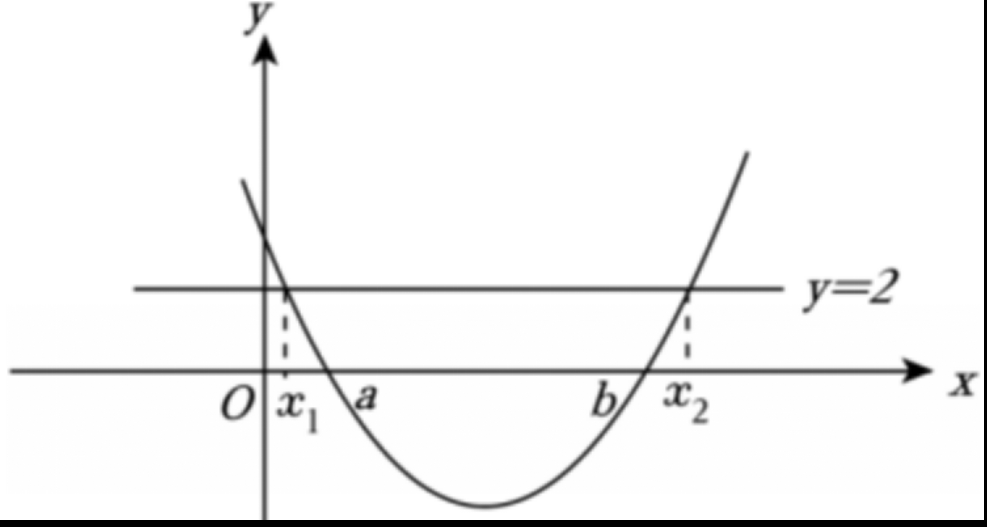
\includegraphics[width=0.42\textwidth]{figures/gao100_q16_parabola.png}
\end{center}
\step{所以数形结合得 $x_1<a<b<x_2$．故选 $B$.}
\solend
\fi

\end{enumerate}

\bigsec{三、解答题}

\begin{enumerate}
\setcounter{enumi}{16}

\item 已知集合 $A=\{x\mid3<x\leqslant6\}$，$B=\{x\mid m\leqslant x\leqslant2m+1\}$.

（1）若 $m=2$，求 $A\cap B$、$A\cup B$；

（2）若 $x\in B$ 是 $x\in A$ 的必要条件，求实数 $m$ 的取值范围.

\ansspace*[9]

\ifanswer
\solbegin
\stepm{（1）}{若 $m=2$，则 $B=\{x\mid2\leqslant x\leqslant5\}$，因为 $A=\{x\mid3<x\leqslant6\}$，}
\step{所以 $A\cap B=\{x\mid3<x\leqslant5\}$，$A\cup B=\{x\mid2\leqslant x\leqslant6\}$.}
\stepm{（2）}{因为 $x\in B$ 是 $x\in A$ 的必要条件，所以 $A\subseteq B$，}
\step{所以 $\begin{cases}m\leqslant3\\ 2m+1\geqslant6\end{cases}$，所以 $\dfrac52\leqslant m\leqslant3$，所以实数 $m$ 的取值范围为 $\left[\dfrac52,3\right]$.}
\solend
\fi

\item 求关于 $x$ 的不等式 $3ax^2-(3a+2)x+2<0\,(a\in R)$ 的解集.

\ansspace*[10]

\ifanswer
\solbegin
\step{当 $a=0$ 时，不等式化为 $-2x+2<0$，解得 $x>1$，}
\step{当 $a\neq0$ 时，方程 $3ax^2-(3a+2)x+2=0$ 的两根分别为 $1$，$\dfrac2{3a}$}
\step{当 $\dfrac2{3a}=1$，即 $a=\dfrac23$ 时，不等式化为 $(x-1)^2<0$，不等式无解，}
\step{当 $\dfrac2{3a}<1$，即 $a>\dfrac23$ 时，不等式解集为 $\left(\dfrac2{3a},1\right)$，}
\step{当 $0<a<\dfrac23$ 时，$\dfrac2{3a}>1$，不等式的解集为 $\left(1,\dfrac2{3a}\right)$，}
\step{当 $a<0$ 时，不等式的解集为 $\left(-\infty,\dfrac2{3a}\right)\cup(1,+\infty)$，}
\step{综上，当 $a=0$ 时，不等式的解集为 $(1,+\infty)$，}
\step{当 $a=\dfrac23$ 时，不等式的解集为 $\varnothing$，}
\step{当 $a>\dfrac23$ 时，不等式解集为 $\left(\dfrac2{3a},1\right)$，}
\step{当 $0<a<\dfrac23$ 时，不等式的解集为 $\left(1,\dfrac2{3a}\right)$，}
\step{当 $a<0$ 时，不等式的解集为 $\left(-\infty,\dfrac2{3a}\right)\cup(1,+\infty)$.}
\solend
\fi

\item 设对于任意实数 $x$，不等式 $\lvert x+1\rvert+\lvert x-1\rvert\geqslant m$ 恒成立.

（1）求 $m$ 的取值范围；

（2）当 $m$ 取最大值时，解关于 $x$ 的不等式 $\lvert x-3\rvert-2x\leqslant2m-2$.

\ansspace*[9]

\ifanswer
\solbegin
\stepm{（1）}{设函数 $f(x)=\lvert x+1\rvert+\lvert x-1\rvert$，则 $f(x)=\begin{cases}-2x,&x\leqslant-1\\ 2,&-1<x<1\\ 2x,&x\geqslant1\end{cases}$，}
\step{当 $x\leqslant-1$ 时，$f(x)$ 有最小值 2；}
\step{当 $-1<x<1$ 时，$f(x)=2$；}
\step{当 $x\geqslant1$ 时，$f(x)$ 有最小值 2；}
\step{因为对于任意实数 $x$，不等式 $\lvert x+1\rvert+\lvert x-1\rvert\geqslant m$ 恒成立，}
\step{所以 $m\leqslant2$，即 $m$ 的取值范围为 $(-\infty,2]$；}
\stepm{（2）}{由（1）得 $m$ 的最大值为 2，所以原不等式为 $\lvert x-3\rvert\leqslant2x+2$，}
\step{即 $-2x-2\leqslant x-3\leqslant2x+2$，解得 $x\geqslant\dfrac13$，}
\step{所以原不等式的解集为 $\left\{x\mid x\geqslant\dfrac13\right\}$.}
\solend
\fi

\item 某轮船公司的一艘轮船每小时花费的燃料费与轮船航行速度的平方成正比，比例系数为 $k$．轮船的最大速度为 18 海里/小时．当船速为 10 海里/小时，它的燃料费是每小时 120 元，其余航行运作费用（不论速度如何）总计是每小时 120 元．假定运行过程中轮船以速度 $v$ 匀速航行.

（1）求 $k$ 的值及每小时的最大总费用 $H$；

（2）求该轮船航行 100 海里的总费用 $W$（燃料费＋其余航行运作费用）的最小值.

\ansspace*[10]

\ifanswer
\solbegin
\stepm{（1）}{由题意，每小时燃料费为 $h(v)=kv^2$，$0<v\leqslant18$，}
\step{已知 $v=10$ 时，燃料费每小时 120 元，则 $k\cdot10^2=120$，得 $k=1.2$，}
\step{每小时总费用 $h(v)=kv^2+120=1.2v^2+120$，}
\step{$h(v)$ 是关于 $v$ 的增函数，$v$ 最大为 18，}
\step{所以 $H=h(18)=1.2\times18^2+120=508.8$ 元.}
\stepm{（2）}{航行时间 $t=\dfrac{100}v$ 小时，}
\step{$W(v)=h(v)\cdot t=(1.2v^2+120)\cdot\dfrac{100}v,0<v\leqslant18=120v+\dfrac{12000}v$，}
\step{利用均值不等式 $120v+\dfrac{12000}v\geqslant2\sqrt{120v\cdot\dfrac{12000}v}=2\times1200=2400$，}
\step{当且仅当 $120v=\dfrac{12000}v$，即 $v=10$ 时取等号，}
\step{$v=10\leqslant18$，在速度范围内，可取到等号，所以总费用最小值为 2400 元.}
\solend
\fi

\item 已知 $A$ 是 $R$ 的非空真子集，如果对任意 $x$、$y\in A$，都有 $x+y\in A$，$xy\in A$，则称 $A$ 是封闭集.

（1）判断集合 $B=\{0\}$，$C=\{-1,0,1\}$ 是否为封闭集，并说明理由；

（2）判断以下两个命题的真假，并说明理由；

命题 $p$：若非空集合 $A_1$、$A_2$ 是封闭集，则 $A_1\cup A_2$ 也是封闭集；

命题 $q$：非空集合 $A_1$、$A_2$ 是封闭集，则 $A_1\cap A_2\neq\varnothing$ 是 $A_1\cap A_2$ 是封闭集的充要条件；

（3）若非空集合 $A$ 是封闭集合，设全集为 $R$，求证：$A$ 的补集不是封闭集.

\ansspace*[13]

\ifanswer
\solbegin
\stepm{（1）}{$B=\{0\}$ 是封闭集，$C=\{-1,0,1\}$ 不是封闭集，理由如下：}
\step{对于集合 $B=\{0\}$，因为 $0+0=0\in B$，$0\times0=0\in B$，}
\step{所以 $B=\{0\}$ 是封闭集；}
\step{对于集合 $C=\{-1,0,1\}$，因为 $-1+(-1)=-2\notin C$，$1+1=2\notin C$，}
\step{所以集合 $C=\{-1,0,1\}$ 不是封闭集.}
\stepm{（2）}{命题 $p$ 是假命题，命题 $q$ 是真命题，理由如下：}
\step{对命题 $p$：令 $A_1=\{x\mid x=2k,k\in Z\}$，$A_2=\{x\mid x=3k,k\in Z\}$，}
\step{令 $x_1=2k_1$，$y_1=2k_2$，$k_1$、$k_2\in Z$，}
\step{则 $x_1+y_1=2(k_1+k_2)\in A_1$，$x_1y_1=2(2k_1k_2)\in A_1$，}
\step{因此集合 $A_1$ 是封闭集，同理集合 $A_2$ 也是封闭集，}
\step{取 $x_2=2$，$y_2=3$，则 $x_2$、$y_2\in(A_1\cup A_2)$，而 $x_2+y_2=5\notin(A_1\cup A_2)$，}
\step{因此集合 $A_1\cup A_2$ 不是封闭集，命题 $p$ 是假命题；}
\step{对于命题 $q$：若 $A_1\cap A_2\neq\varnothing$，不妨令 $a$、$b\in(A_1\cap A_2)$，}
\step{则有 $a$、$b\in A_1$，又集合 $A_1$ 是封闭集，则 $a+b\in A_1$，$ab\in A_1$，}
\step{同理 $a+b\in A_2$，$ab\in A_2$，因此 $a+b\in(A_1\cap A_2)$，$ab\in(A_1\cap A_2)$，}
\step{所以 $A_1\cap A_2$ 是封闭集；}
\step{反之，若 $A_1\cap A_2$ 是封闭集，则 $A_1\cap A_2$ 是非空集合，即 $A_1\cap A_2\neq\varnothing$，}
\step{所以 $A_1\cap A_2$ 是 $A_1\cap A_2$ 是封闭集的充要条件，命题 $q$ 是真命题.}
\stepm{（3）}{非空集合 $A$ 是封闭集合，当 $A=R$ 时，$\overline A=\varnothing$，因此 $\overline A$ 不是封闭集合；}
\step{当 $A\neq R$ 时，假设 $\overline A$ 是封闭集合，}
\step{设 $0\in A$，在 $\overline A$ 中任取一个 $x$，$x\neq0$，则 $-x\in A$，}
\step{否则 $-x\in\overline A$，此时 $x+(-x)=0\in\overline A$，与 $0\in A$ 矛盾，}
\step{因此 $(-x)^2\in A$，$x^2\in\overline A$，而 $(-x)^2=x^2$，与 $A\cap\overline A=\varnothing$ 矛盾，}
\step{则当 $0\in A$ 时，则 $\overline A$ 不是封闭集合，同理当 $0\in\overline A$ 时，$\overline A$ 不是封闭集合，}
\step{所以 $A$ 的补集不是封闭集.}
\solend
\fi

\end{enumerate}

\end{document}
"
% 紧凑版：xelatex "\def\iscompact{1}% 高一100_南洋中学_10月月考.tex
%   —— 高一上数学“2026-2027 年南洋中学高一上 10 月月考”（讲评版）
% 试卷版：xelatex 高一100_南洋中学_10月月考.tex
% 答案版：xelatex "\def\isanswer{1}\input{高一100_南洋中学_10月月考.tex}"
% 紧凑版：xelatex "\def\iscompact{1}\input{高一100_南洋中学_10月月考.tex}"
%
% 原始材料：微信公众号“魔都数学加油站”文章，连载“27学年高一100”；
% 原文标题“27学年高一100——2026-2027年上海市南洋中学高一上10月月考”；
% 原文链接：https://mp.weixin.qq.com/s/uXLyt6VHraW4hSpDwnZDuQ。
% 正文为 10 张 PNG 页（`原图/高一100_南洋中学_10月月考/01..10.png`），
% 尺寸混排（第 2、4—9 页为 4762×6735，第 1、3、10 页为 2560×3620），按页序读取。
%
% 篇幅与题号：原卷自第 3 题起编号（第 1、2 题不在原文内）。填空题 3—12（10 题）、
% 选择题 13—16（4 题）、解答题 17—21（5 题），共 19 题。
%
% 讲评版：全部 19 题均印【解析】，其中第 13—16 题的答案在解析末句
% “故选 $C$／$B$／$D$／$B$”（题干括号内未印答案）。第 16 题解析带一幅
% 抛物线与 $y=2$ 的示意图，自原图裁切、去粉色水印后转灰度，三版都出。
%
% 副标题：原卷未印副标题。本稿按内容标作“集合与常用逻辑用语、不等式”。
%
% 原卷笔误/存疑（均照录未改，正文对应处另有 % 注）：无。
%
% 与原卷的排版差异：
%   ① 原卷每题下直接印【解析】，本稿按全稿惯例将答案与解析置于答案版；
%   ② 原卷未印副标题，本稿补出；填空横线统一排 \blankline[4.4em]；
%   ③ 原卷数集记号排斜体 $R$、$Z$、$\mathit N$，本稿按全稿惯例改用 $\R$、$\Z$、$\N$；
%   ④ 解答题按惯例加 \ansspace；选择题括号排 \mbox{（\quad）}；
%   ⑤ 第 16 题的示意图原卷排在解析行右侧，本稿改排为解析后的居中图。
%
% 行数核对：逐题数 \step/\stepm 条数，合计 117 条（Q3：2；Q4：5；Q5：7；Q6：3；Q7：3；
% Q8：4；Q9：2；Q10：4；Q11：6；Q12：3；Q13：7；Q14：3；Q15：5；Q16：3；Q17：5；
% Q18：11；Q19：9；Q20：10；Q21：25）。全卷 19 题均印【解析】。
% 原卷解析的换行按语意合并，未逐行强拆。
%
\documentclass[a4paper,11pt]{article}
\usepackage{common}
\begin{document}

\examtitlest[7]{2026--2027 年南洋中学高一上 10 月月考}{集合与常用逻辑用语、不等式}

\bigsec{一、填空题}

\begin{enumerate}
\setcounter{enumi}{2}

\item 不等式 $\dfrac{x-6}{x+1}\geqslant0$ 的解集为\blankline[4.4em].

\ifanswer
\solbegin
\step{不等式 $\dfrac{x-6}{x+1}\geqslant0$ 等价于 $\begin{cases}(x-6)(x+1)\geqslant0\\ x+1\neq0\end{cases}$，即 $x<-1$ 或 $x\geqslant6$，}
\step{故解集为 $(-\infty,-1)\cup[6,+\infty)$.}
\solend
\fi

\item 已知关于 $x$ 的不等式 $ax^2+bx+c>0$ 的解集是 $(1,3)$，则关于 $x$ 的不等式 $ax^2-bx+c\leqslant0$ 的解集为\blankline[4.4em].

\ifanswer
\solbegin
\step{由已知得 $a<0$，且 $1$，$3$ 是方程 $ax^2+bx+c=0$ 的根，}
\step{所以 $\begin{cases}1+3=-\dfrac ba\\[2pt] 1\times3=\dfrac ca\end{cases}$，所以 $\begin{cases}b=-4a\\ c=3a\end{cases}$，}
\step{所以 $ax^2-bx+c\leqslant0$ 可变形为 $ax^2+4ax+3a\leqslant0$，}
\step{因为 $a<0$，所以 $x^2+4x+3\geqslant0$，解得 $x\leqslant-3$ 或 $x\geqslant-1$，}
\step{所以不等式的解集为 $(-\infty,-3]\cup[-1,+\infty)$.}
\solend
\fi

\item 不等式 $\lvert x+2\rvert+\lvert 2x-1\rvert\geqslant3$ 的解集为\blankline[4.4em].

\ifanswer
\solbegin
\step{当 $x\leqslant-2$ 时，$x+2\leqslant0$，$2x-1<0$，}
\step{所以 $\lvert x+2\rvert+\lvert 2x-1\rvert=-x-2-2x+1\geqslant3$，解得 $x\leqslant-\dfrac43$；}
\step{当 $-2<x<\dfrac12$ 时，$x+2>0$，$2x-1<0$，}
\step{所以 $\lvert x+2\rvert+\lvert 2x-1\rvert=x+2-2x+1\geqslant3$，解得 $x\leqslant0$；}
\step{当 $x\geqslant\dfrac12$ 时，$x+2>0$，$2x-1\geqslant0$，}
\step{所以 $\lvert x+2\rvert+\lvert 2x-1\rvert=x+2+2x-1\geqslant3$，解得 $x\geqslant\dfrac23$；}
\step{所以原不等式的解集为 $\left\{x\mid x\leqslant0\right.$ 或 $\left.x\geqslant\dfrac23\right\}$.}
\solend
\fi

\item 若正数 $x$、$y$ 满足 $x+2y=2$，则 $\dfrac1x+\dfrac2y$ 的最小值是\blankline[4.4em].

\ifanswer
\solbegin
\step{因为 $x>0$，$y>0$，且 $x+2y=2$，}
\step{所以 $\dfrac1x+\dfrac2y=\dfrac12\left(\dfrac1x+\dfrac2y\right)(x+2y)=\dfrac12\left(5+\dfrac{2y}x+\dfrac{2x}y\right)\geqslant\dfrac12\left(5+2\sqrt{\dfrac{2y}x\cdot\dfrac{2x}y}\right)=\dfrac92$.}
\step{当且仅当 $\begin{cases}x+2y=2\\ \dfrac{2y}x=\dfrac{2x}y\end{cases}$，即 $x=y=\dfrac23$ 时取等号，故最小值为 $\dfrac92$.}
\solend
\fi

\item 已知 $\alpha:x\leqslant2$ 或 $x>3$，$\beta:x\leqslant m+5$ 或 $x>-m$，若 $\alpha$ 是 $\beta$ 的必要非充分条件，则实数 $m$ 的取值范围是\blankline[4.4em].

\ifanswer
\solbegin
\step{设 $A=\{x\mid x\leqslant2$ 或 $x>3\}$，$B=\{x\mid x\leqslant m+5$ 或 $x>-m\}$，则 $B\subset A$，}
\step{则 $m+5\leqslant2$ 且 $-m\geqslant3$（等号不能同时取得），则 $m<-3$，}
\step{则实数 $m$ 的取值范围是 $(-\infty,-3)$.}
\solend
\fi

\item 已知集合 $A=\{x\mid-1\leqslant x\leqslant3\}$，$B=\{x\mid ax+1>0\}$ 满足 $A\subseteq B$，则实数 $a$ 的取值范围为\blankline[4.4em].

\ifanswer
\solbegin
\step{当 $a=0$ 时，$B=R$，显然符合题意，}
\step{当 $a>0$ 时，$B=\left\{x\mid x>-\dfrac1a\right\}$，则 $-\dfrac1a<-1$，解得 $a<1$，所以 $0<a<1$，}
\step{当 $a<0$ 时，$B=\left\{x\mid x<-\dfrac1a\right\}$，则 $-\dfrac1a>3$，解得 $a>-\dfrac13$，所以 $-\dfrac13<a<0$，}
\step{综上所述，实数 $a$ 的取值范围为 $\left(-\dfrac13,1\right)$.}
\solend
\fi

\item 设集合 $A=\{x\mid3x-1<m\}$，若 $1\in A$ 且 $2\notin A$，则实数 $m$ 的取值范围是\blankline[4.4em].

\ifanswer
\solbegin
\step{因为集合 $A=\{x\mid3x-1<m\}$，若 $1\in A$ 且 $2\notin A$，}
\step{则 $3\times1-1<m$ 且 $3\times2-1\geqslant m$，解得 $2<m\leqslant5$.}
\solend
\fi

\item 若 $M=\left\{x\mid x=m+\dfrac16,m\in Z\right\},N=\left\{x\mid x=\dfrac n2-\dfrac13,n\in Z\right\}$，\newline $P=\left\{x\mid x=\dfrac p2+\dfrac16,p\in Z\right\}$，则 $M$、$N$、$P$ 的关系为\blankline[4.4em].

\ifanswer
\solbegin
\step{$M=\left\{x\mid x=m+\dfrac16=\dfrac{6m+1}6=\dfrac{3\cdot2m+1}6,m\in Z\right\}$，}
\step{$N=\left\{x\mid x=\dfrac n2-\dfrac13=\dfrac{3(n-1)+1}6,n\in Z\right\}=\left\{x\mid x=\dfrac{3k+1}6,k\in Z\right\}$，}
\step{$P=\left\{x\mid x=\dfrac p2+\dfrac16=\dfrac{3p+1}6,p\in Z\right\}$，}
\step{故 $M\subset N=P$.}
\solend
\fi

\item 已知命题 $p:x<-2$ 或 $x>3$，命题 $q:x<3m+1$ 或 $x>m+2$，若 $p$ 是 $q$ 的充分非必要条件，则实数 $m$ 的取值范围是\blankline[4.4em].

\ifanswer
\solbegin
\step{设 $A=\{x\mid x<-2$ 或 $x>3\}$，$B=\{x\mid x<3m+1$ 或 $x>m+2\}$，}
\step{若 $p$ 是 $q$ 的充分非必要条件，则 $A\subset B$，}
\step{当 $3m+1\geqslant m+2$，即 $m\geqslant\dfrac12$ 时，显然有 $A\subset B$，}
\step{当 $3m+1<m+2$，即 $m<\dfrac12$ 时，}
\step{由 $A\subset B$，则 $\begin{cases}m+2\leqslant3\\ 3m+1\geqslant-2\end{cases}$（等号不同时成立），即 $-1\leqslant m<\dfrac12$.}
\step{综上，实数 $m$ 的取值范围是 $[-1,+\infty)$.}
\solend
\fi

\item 对于一个有限集 $A$，一般都可以找到两个非空数集 $A_1$ 和 $A_2$，满足 $A_1\cap A_2=\varnothing$，且 $A_1\cup A_2=A$，记集合 $\{A_1,A_2\}$ 为 $A$ 的一个“划分集”．若 $A$ 中有 $n(n\geqslant2,n\in\N)$ 个元素，则不同的“划分集”共有\blankline[4.4em]个(用含 $n$ 的表达式填空).

\ifanswer
\solbegin
\step{集合中的每个元素都有属于 $A_1$ 或属于 $A_2$ 两种情况，故共有 $2^n$ 种情况，}
\step{排除全都属于 $A_1$ 或 $A_2$ 的两种情况，考虑对称情况，}
\step{故不同的“划分集”共有 $\dfrac12(2^n-2)=2^{n-1}-1$ 个.}
\solend
\fi

\end{enumerate}

\bigsec{二、选择题}

\begin{enumerate}
\setcounter{enumi}{12}

\item 下列命题中正确的\mbox{（\quad）}

\keepwithprev
A. $\varnothing$ 与 $\{0\}$ 表示同一个集合

B. 方程 $\{x\mid(x-2)^2(x-3)=0\}$ 的所有解的集合可表示为 $\{2,2,3\}$

C. 由 3，4，5 组成的集合可表示为 $\{3,4,5\}$ 或 $\{4,5,3\}$

D. 很小的实数可以构成集合.

\ifanswer
\solbegin
\step{对于 $A$，$\{0\}$ 中有一个元素 0，$\varnothing$ 中无任何元素，故 $\varnothing$ 与 $\{0\}$ 不是同一个集合，}
\step{故 $A$ 错误；}
\step{对于 $B$，$\{2,2,3\}$ 不满足集合元素的互异性，故 $B$ 错误；}
\step{对于 $C$，由集合的无序性，得由 3，4，5 组成的集合可表示为 $\{3,4,5\}$ 或 $\{4,5,3\}$，}
\step{故 $C$ 正确；}
\step{对于 $D$，由集合的确定性，很小的实数不能构成集合，故 $D$ 错误.}
\step{故选 $C$.}
\solend
\fi

\item 已知 $a\in R$，则“$\dfrac1a<1$”是“$a>1$”的\mbox{（\quad）}条件.

\keepwithprev
A. 充分非必要\qquad B. 必要非充分

C. 充要\qquad D. 既非充分又非必要

\ifanswer
\solbegin
\step{解 $\dfrac1a<1$，得 $a<0$ 或 $a>1$，}
\step{由 $a<0$ 或 $a>1$ 得不出 $a>1$，由 $a>1$ 得出 $a<0$ 或 $a>1$，}
\step{所以“$\dfrac1a<1$”是“$a>1$”的必要不充分条件．故选 $B$.}
\solend
\fi

\item 若命题“存在 $x_0\in R$ 使得 $ax_0^2+2ax_0+1\leqslant0$”是假命题，则实数 $a$ 的取值范围为\mbox{（\quad）}

\keepwithprev
A. $a<0$ 或 $a\geqslant1$\qquad B. $a\leqslant0$ 或 $a\geqslant1$\qquad C. $0<a<1$\qquad D. $0\leqslant a<1$

\ifanswer
\solbegin
\step{命题“存在 $x_0\in R$ 使得 $ax_0^2+2ax_0+1\leqslant0$”是假命题，}
\step{则 $\forall x\in R$，$ax^2+2ax+1>0$ 恒成立，}
\step{当 $a=0$ 时，满足题意，}
\step{当 $a\neq0$ 时，$\begin{cases}a>0\\ \Delta=4a^2-4a<0\end{cases}$，解得 $0<a<1$，}
\step{综上所述，实数 $a$ 的取值范围为 $\{a\mid0\leqslant a<1\}$．故选 $D$.}
\solend
\fi

\item 已知实数 $a<b$，关于 $x$ 的不等式 $x^2-(a+b)x+ab-2<0$ 的解集为 $(x_1,x_2)$，则实数 $a$、$b$、$x_1$、$x_2$ 从小到大的排列是\mbox{（\quad）}

\keepwithprev
A. $a<x_1<x_2<b$\qquad B. $x_1<a<b<x_2$\qquad C. $a<x_1<b<x_2$\qquad D. $x_1<a<x_2<b$

\ifanswer
\solbegin
\step{因为实数 $a<b$，不等式 $x^2-(a+b)x+ab-2<0$ 可化为 $(x-a)(x-b)<2$，}
\step{又其解集为 $(x_1,x_2)$，所以作出 $y=(x-a)(x-b)$ 与 $y=2$ 的图象如下：}
\begin{center}
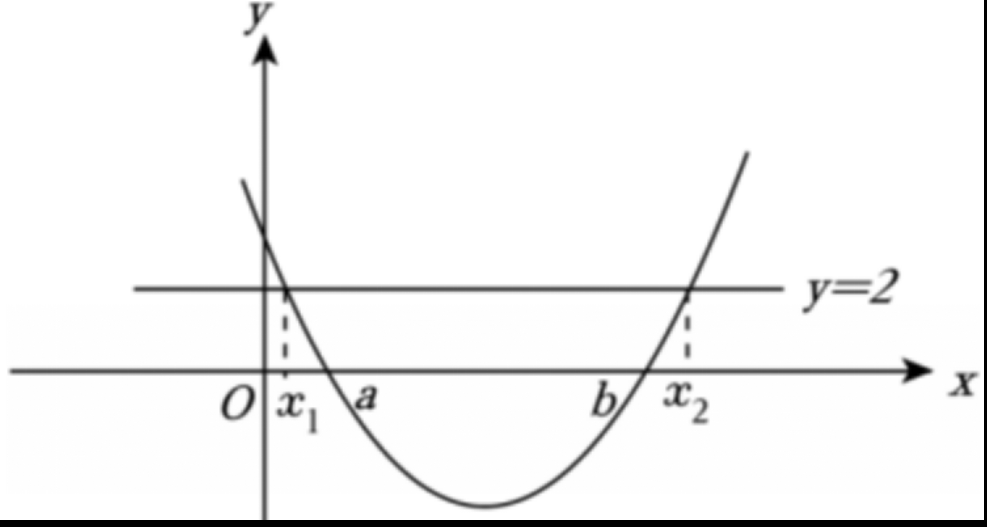
\includegraphics[width=0.42\textwidth]{figures/gao100_q16_parabola.png}
\end{center}
\step{所以数形结合得 $x_1<a<b<x_2$．故选 $B$.}
\solend
\fi

\end{enumerate}

\bigsec{三、解答题}

\begin{enumerate}
\setcounter{enumi}{16}

\item 已知集合 $A=\{x\mid3<x\leqslant6\}$，$B=\{x\mid m\leqslant x\leqslant2m+1\}$.

（1）若 $m=2$，求 $A\cap B$、$A\cup B$；

（2）若 $x\in B$ 是 $x\in A$ 的必要条件，求实数 $m$ 的取值范围.

\ansspace*[9]

\ifanswer
\solbegin
\stepm{（1）}{若 $m=2$，则 $B=\{x\mid2\leqslant x\leqslant5\}$，因为 $A=\{x\mid3<x\leqslant6\}$，}
\step{所以 $A\cap B=\{x\mid3<x\leqslant5\}$，$A\cup B=\{x\mid2\leqslant x\leqslant6\}$.}
\stepm{（2）}{因为 $x\in B$ 是 $x\in A$ 的必要条件，所以 $A\subseteq B$，}
\step{所以 $\begin{cases}m\leqslant3\\ 2m+1\geqslant6\end{cases}$，所以 $\dfrac52\leqslant m\leqslant3$，所以实数 $m$ 的取值范围为 $\left[\dfrac52,3\right]$.}
\solend
\fi

\item 求关于 $x$ 的不等式 $3ax^2-(3a+2)x+2<0\,(a\in R)$ 的解集.

\ansspace*[10]

\ifanswer
\solbegin
\step{当 $a=0$ 时，不等式化为 $-2x+2<0$，解得 $x>1$，}
\step{当 $a\neq0$ 时，方程 $3ax^2-(3a+2)x+2=0$ 的两根分别为 $1$，$\dfrac2{3a}$}
\step{当 $\dfrac2{3a}=1$，即 $a=\dfrac23$ 时，不等式化为 $(x-1)^2<0$，不等式无解，}
\step{当 $\dfrac2{3a}<1$，即 $a>\dfrac23$ 时，不等式解集为 $\left(\dfrac2{3a},1\right)$，}
\step{当 $0<a<\dfrac23$ 时，$\dfrac2{3a}>1$，不等式的解集为 $\left(1,\dfrac2{3a}\right)$，}
\step{当 $a<0$ 时，不等式的解集为 $\left(-\infty,\dfrac2{3a}\right)\cup(1,+\infty)$，}
\step{综上，当 $a=0$ 时，不等式的解集为 $(1,+\infty)$，}
\step{当 $a=\dfrac23$ 时，不等式的解集为 $\varnothing$，}
\step{当 $a>\dfrac23$ 时，不等式解集为 $\left(\dfrac2{3a},1\right)$，}
\step{当 $0<a<\dfrac23$ 时，不等式的解集为 $\left(1,\dfrac2{3a}\right)$，}
\step{当 $a<0$ 时，不等式的解集为 $\left(-\infty,\dfrac2{3a}\right)\cup(1,+\infty)$.}
\solend
\fi

\item 设对于任意实数 $x$，不等式 $\lvert x+1\rvert+\lvert x-1\rvert\geqslant m$ 恒成立.

（1）求 $m$ 的取值范围；

（2）当 $m$ 取最大值时，解关于 $x$ 的不等式 $\lvert x-3\rvert-2x\leqslant2m-2$.

\ansspace*[9]

\ifanswer
\solbegin
\stepm{（1）}{设函数 $f(x)=\lvert x+1\rvert+\lvert x-1\rvert$，则 $f(x)=\begin{cases}-2x,&x\leqslant-1\\ 2,&-1<x<1\\ 2x,&x\geqslant1\end{cases}$，}
\step{当 $x\leqslant-1$ 时，$f(x)$ 有最小值 2；}
\step{当 $-1<x<1$ 时，$f(x)=2$；}
\step{当 $x\geqslant1$ 时，$f(x)$ 有最小值 2；}
\step{因为对于任意实数 $x$，不等式 $\lvert x+1\rvert+\lvert x-1\rvert\geqslant m$ 恒成立，}
\step{所以 $m\leqslant2$，即 $m$ 的取值范围为 $(-\infty,2]$；}
\stepm{（2）}{由（1）得 $m$ 的最大值为 2，所以原不等式为 $\lvert x-3\rvert\leqslant2x+2$，}
\step{即 $-2x-2\leqslant x-3\leqslant2x+2$，解得 $x\geqslant\dfrac13$，}
\step{所以原不等式的解集为 $\left\{x\mid x\geqslant\dfrac13\right\}$.}
\solend
\fi

\item 某轮船公司的一艘轮船每小时花费的燃料费与轮船航行速度的平方成正比，比例系数为 $k$．轮船的最大速度为 18 海里/小时．当船速为 10 海里/小时，它的燃料费是每小时 120 元，其余航行运作费用（不论速度如何）总计是每小时 120 元．假定运行过程中轮船以速度 $v$ 匀速航行.

（1）求 $k$ 的值及每小时的最大总费用 $H$；

（2）求该轮船航行 100 海里的总费用 $W$（燃料费＋其余航行运作费用）的最小值.

\ansspace*[10]

\ifanswer
\solbegin
\stepm{（1）}{由题意，每小时燃料费为 $h(v)=kv^2$，$0<v\leqslant18$，}
\step{已知 $v=10$ 时，燃料费每小时 120 元，则 $k\cdot10^2=120$，得 $k=1.2$，}
\step{每小时总费用 $h(v)=kv^2+120=1.2v^2+120$，}
\step{$h(v)$ 是关于 $v$ 的增函数，$v$ 最大为 18，}
\step{所以 $H=h(18)=1.2\times18^2+120=508.8$ 元.}
\stepm{（2）}{航行时间 $t=\dfrac{100}v$ 小时，}
\step{$W(v)=h(v)\cdot t=(1.2v^2+120)\cdot\dfrac{100}v,0<v\leqslant18=120v+\dfrac{12000}v$，}
\step{利用均值不等式 $120v+\dfrac{12000}v\geqslant2\sqrt{120v\cdot\dfrac{12000}v}=2\times1200=2400$，}
\step{当且仅当 $120v=\dfrac{12000}v$，即 $v=10$ 时取等号，}
\step{$v=10\leqslant18$，在速度范围内，可取到等号，所以总费用最小值为 2400 元.}
\solend
\fi

\item 已知 $A$ 是 $R$ 的非空真子集，如果对任意 $x$、$y\in A$，都有 $x+y\in A$，$xy\in A$，则称 $A$ 是封闭集.

（1）判断集合 $B=\{0\}$，$C=\{-1,0,1\}$ 是否为封闭集，并说明理由；

（2）判断以下两个命题的真假，并说明理由；

命题 $p$：若非空集合 $A_1$、$A_2$ 是封闭集，则 $A_1\cup A_2$ 也是封闭集；

命题 $q$：非空集合 $A_1$、$A_2$ 是封闭集，则 $A_1\cap A_2\neq\varnothing$ 是 $A_1\cap A_2$ 是封闭集的充要条件；

（3）若非空集合 $A$ 是封闭集合，设全集为 $R$，求证：$A$ 的补集不是封闭集.

\ansspace*[13]

\ifanswer
\solbegin
\stepm{（1）}{$B=\{0\}$ 是封闭集，$C=\{-1,0,1\}$ 不是封闭集，理由如下：}
\step{对于集合 $B=\{0\}$，因为 $0+0=0\in B$，$0\times0=0\in B$，}
\step{所以 $B=\{0\}$ 是封闭集；}
\step{对于集合 $C=\{-1,0,1\}$，因为 $-1+(-1)=-2\notin C$，$1+1=2\notin C$，}
\step{所以集合 $C=\{-1,0,1\}$ 不是封闭集.}
\stepm{（2）}{命题 $p$ 是假命题，命题 $q$ 是真命题，理由如下：}
\step{对命题 $p$：令 $A_1=\{x\mid x=2k,k\in Z\}$，$A_2=\{x\mid x=3k,k\in Z\}$，}
\step{令 $x_1=2k_1$，$y_1=2k_2$，$k_1$、$k_2\in Z$，}
\step{则 $x_1+y_1=2(k_1+k_2)\in A_1$，$x_1y_1=2(2k_1k_2)\in A_1$，}
\step{因此集合 $A_1$ 是封闭集，同理集合 $A_2$ 也是封闭集，}
\step{取 $x_2=2$，$y_2=3$，则 $x_2$、$y_2\in(A_1\cup A_2)$，而 $x_2+y_2=5\notin(A_1\cup A_2)$，}
\step{因此集合 $A_1\cup A_2$ 不是封闭集，命题 $p$ 是假命题；}
\step{对于命题 $q$：若 $A_1\cap A_2\neq\varnothing$，不妨令 $a$、$b\in(A_1\cap A_2)$，}
\step{则有 $a$、$b\in A_1$，又集合 $A_1$ 是封闭集，则 $a+b\in A_1$，$ab\in A_1$，}
\step{同理 $a+b\in A_2$，$ab\in A_2$，因此 $a+b\in(A_1\cap A_2)$，$ab\in(A_1\cap A_2)$，}
\step{所以 $A_1\cap A_2$ 是封闭集；}
\step{反之，若 $A_1\cap A_2$ 是封闭集，则 $A_1\cap A_2$ 是非空集合，即 $A_1\cap A_2\neq\varnothing$，}
\step{所以 $A_1\cap A_2$ 是 $A_1\cap A_2$ 是封闭集的充要条件，命题 $q$ 是真命题.}
\stepm{（3）}{非空集合 $A$ 是封闭集合，当 $A=R$ 时，$\overline A=\varnothing$，因此 $\overline A$ 不是封闭集合；}
\step{当 $A\neq R$ 时，假设 $\overline A$ 是封闭集合，}
\step{设 $0\in A$，在 $\overline A$ 中任取一个 $x$，$x\neq0$，则 $-x\in A$，}
\step{否则 $-x\in\overline A$，此时 $x+(-x)=0\in\overline A$，与 $0\in A$ 矛盾，}
\step{因此 $(-x)^2\in A$，$x^2\in\overline A$，而 $(-x)^2=x^2$，与 $A\cap\overline A=\varnothing$ 矛盾，}
\step{则当 $0\in A$ 时，则 $\overline A$ 不是封闭集合，同理当 $0\in\overline A$ 时，$\overline A$ 不是封闭集合，}
\step{所以 $A$ 的补集不是封闭集.}
\solend
\fi

\end{enumerate}

\end{document}
"
%
% 原始材料：微信公众号“魔都数学加油站”文章，连载“27学年高一100”；
% 原文标题“27学年高一100——2026-2027年上海市南洋中学高一上10月月考”；
% 原文链接：https://mp.weixin.qq.com/s/uXLyt6VHraW4hSpDwnZDuQ。
% 正文为 10 张 PNG 页（`原图/高一100_南洋中学_10月月考/01..10.png`），
% 尺寸混排（第 2、4—9 页为 4762×6735，第 1、3、10 页为 2560×3620），按页序读取。
%
% 篇幅与题号：原卷自第 3 题起编号（第 1、2 题不在原文内）。填空题 3—12（10 题）、
% 选择题 13—16（4 题）、解答题 17—21（5 题），共 19 题。
%
% 讲评版：全部 19 题均印【解析】，其中第 13—16 题的答案在解析末句
% “故选 $C$／$B$／$D$／$B$”（题干括号内未印答案）。第 16 题解析带一幅
% 抛物线与 $y=2$ 的示意图，自原图裁切、去粉色水印后转灰度，三版都出。
%
% 副标题：原卷未印副标题。本稿按内容标作“集合与常用逻辑用语、不等式”。
%
% 原卷笔误/存疑（均照录未改，正文对应处另有 % 注）：无。
%
% 与原卷的排版差异：
%   ① 原卷每题下直接印【解析】，本稿按全稿惯例将答案与解析置于答案版；
%   ② 原卷未印副标题，本稿补出；填空横线统一排 \blankline[4.4em]；
%   ③ 原卷数集记号排斜体 $R$、$Z$、$\mathit N$，本稿按全稿惯例改用 $\R$、$\Z$、$\N$；
%   ④ 解答题按惯例加 \ansspace；选择题括号排 \mbox{（\quad）}；
%   ⑤ 第 16 题的示意图原卷排在解析行右侧，本稿改排为解析后的居中图。
%
% 行数核对：逐题数 \step/\stepm 条数，合计 117 条（Q3：2；Q4：5；Q5：7；Q6：3；Q7：3；
% Q8：4；Q9：2；Q10：4；Q11：6；Q12：3；Q13：7；Q14：3；Q15：5；Q16：3；Q17：5；
% Q18：11；Q19：9；Q20：10；Q21：25）。全卷 19 题均印【解析】。
% 原卷解析的换行按语意合并，未逐行强拆。
%
\documentclass[a4paper,11pt]{article}
\usepackage{common}
\begin{document}

\examtitlest[7]{2026--2027 年南洋中学高一上 10 月月考}{集合与常用逻辑用语、不等式}

\bigsec{一、填空题}

\begin{enumerate}
\setcounter{enumi}{2}

\item 不等式 $\dfrac{x-6}{x+1}\geqslant0$ 的解集为\blankline[4.4em].

\ifanswer
\solbegin
\step{不等式 $\dfrac{x-6}{x+1}\geqslant0$ 等价于 $\begin{cases}(x-6)(x+1)\geqslant0\\ x+1\neq0\end{cases}$，即 $x<-1$ 或 $x\geqslant6$，}
\step{故解集为 $(-\infty,-1)\cup[6,+\infty)$.}
\solend
\fi

\item 已知关于 $x$ 的不等式 $ax^2+bx+c>0$ 的解集是 $(1,3)$，则关于 $x$ 的不等式 $ax^2-bx+c\leqslant0$ 的解集为\blankline[4.4em].

\ifanswer
\solbegin
\step{由已知得 $a<0$，且 $1$，$3$ 是方程 $ax^2+bx+c=0$ 的根，}
\step{所以 $\begin{cases}1+3=-\dfrac ba\\[2pt] 1\times3=\dfrac ca\end{cases}$，所以 $\begin{cases}b=-4a\\ c=3a\end{cases}$，}
\step{所以 $ax^2-bx+c\leqslant0$ 可变形为 $ax^2+4ax+3a\leqslant0$，}
\step{因为 $a<0$，所以 $x^2+4x+3\geqslant0$，解得 $x\leqslant-3$ 或 $x\geqslant-1$，}
\step{所以不等式的解集为 $(-\infty,-3]\cup[-1,+\infty)$.}
\solend
\fi

\item 不等式 $\lvert x+2\rvert+\lvert 2x-1\rvert\geqslant3$ 的解集为\blankline[4.4em].

\ifanswer
\solbegin
\step{当 $x\leqslant-2$ 时，$x+2\leqslant0$，$2x-1<0$，}
\step{所以 $\lvert x+2\rvert+\lvert 2x-1\rvert=-x-2-2x+1\geqslant3$，解得 $x\leqslant-\dfrac43$；}
\step{当 $-2<x<\dfrac12$ 时，$x+2>0$，$2x-1<0$，}
\step{所以 $\lvert x+2\rvert+\lvert 2x-1\rvert=x+2-2x+1\geqslant3$，解得 $x\leqslant0$；}
\step{当 $x\geqslant\dfrac12$ 时，$x+2>0$，$2x-1\geqslant0$，}
\step{所以 $\lvert x+2\rvert+\lvert 2x-1\rvert=x+2+2x-1\geqslant3$，解得 $x\geqslant\dfrac23$；}
\step{所以原不等式的解集为 $\left\{x\mid x\leqslant0\right.$ 或 $\left.x\geqslant\dfrac23\right\}$.}
\solend
\fi

\item 若正数 $x$、$y$ 满足 $x+2y=2$，则 $\dfrac1x+\dfrac2y$ 的最小值是\blankline[4.4em].

\ifanswer
\solbegin
\step{因为 $x>0$，$y>0$，且 $x+2y=2$，}
\step{所以 $\dfrac1x+\dfrac2y=\dfrac12\left(\dfrac1x+\dfrac2y\right)(x+2y)=\dfrac12\left(5+\dfrac{2y}x+\dfrac{2x}y\right)\geqslant\dfrac12\left(5+2\sqrt{\dfrac{2y}x\cdot\dfrac{2x}y}\right)=\dfrac92$.}
\step{当且仅当 $\begin{cases}x+2y=2\\ \dfrac{2y}x=\dfrac{2x}y\end{cases}$，即 $x=y=\dfrac23$ 时取等号，故最小值为 $\dfrac92$.}
\solend
\fi

\item 已知 $\alpha:x\leqslant2$ 或 $x>3$，$\beta:x\leqslant m+5$ 或 $x>-m$，若 $\alpha$ 是 $\beta$ 的必要非充分条件，则实数 $m$ 的取值范围是\blankline[4.4em].

\ifanswer
\solbegin
\step{设 $A=\{x\mid x\leqslant2$ 或 $x>3\}$，$B=\{x\mid x\leqslant m+5$ 或 $x>-m\}$，则 $B\subset A$，}
\step{则 $m+5\leqslant2$ 且 $-m\geqslant3$（等号不能同时取得），则 $m<-3$，}
\step{则实数 $m$ 的取值范围是 $(-\infty,-3)$.}
\solend
\fi

\item 已知集合 $A=\{x\mid-1\leqslant x\leqslant3\}$，$B=\{x\mid ax+1>0\}$ 满足 $A\subseteq B$，则实数 $a$ 的取值范围为\blankline[4.4em].

\ifanswer
\solbegin
\step{当 $a=0$ 时，$B=R$，显然符合题意，}
\step{当 $a>0$ 时，$B=\left\{x\mid x>-\dfrac1a\right\}$，则 $-\dfrac1a<-1$，解得 $a<1$，所以 $0<a<1$，}
\step{当 $a<0$ 时，$B=\left\{x\mid x<-\dfrac1a\right\}$，则 $-\dfrac1a>3$，解得 $a>-\dfrac13$，所以 $-\dfrac13<a<0$，}
\step{综上所述，实数 $a$ 的取值范围为 $\left(-\dfrac13,1\right)$.}
\solend
\fi

\item 设集合 $A=\{x\mid3x-1<m\}$，若 $1\in A$ 且 $2\notin A$，则实数 $m$ 的取值范围是\blankline[4.4em].

\ifanswer
\solbegin
\step{因为集合 $A=\{x\mid3x-1<m\}$，若 $1\in A$ 且 $2\notin A$，}
\step{则 $3\times1-1<m$ 且 $3\times2-1\geqslant m$，解得 $2<m\leqslant5$.}
\solend
\fi

\item 若 $M=\left\{x\mid x=m+\dfrac16,m\in Z\right\},N=\left\{x\mid x=\dfrac n2-\dfrac13,n\in Z\right\}$，\newline $P=\left\{x\mid x=\dfrac p2+\dfrac16,p\in Z\right\}$，则 $M$、$N$、$P$ 的关系为\blankline[4.4em].

\ifanswer
\solbegin
\step{$M=\left\{x\mid x=m+\dfrac16=\dfrac{6m+1}6=\dfrac{3\cdot2m+1}6,m\in Z\right\}$，}
\step{$N=\left\{x\mid x=\dfrac n2-\dfrac13=\dfrac{3(n-1)+1}6,n\in Z\right\}=\left\{x\mid x=\dfrac{3k+1}6,k\in Z\right\}$，}
\step{$P=\left\{x\mid x=\dfrac p2+\dfrac16=\dfrac{3p+1}6,p\in Z\right\}$，}
\step{故 $M\subset N=P$.}
\solend
\fi

\item 已知命题 $p:x<-2$ 或 $x>3$，命题 $q:x<3m+1$ 或 $x>m+2$，若 $p$ 是 $q$ 的充分非必要条件，则实数 $m$ 的取值范围是\blankline[4.4em].

\ifanswer
\solbegin
\step{设 $A=\{x\mid x<-2$ 或 $x>3\}$，$B=\{x\mid x<3m+1$ 或 $x>m+2\}$，}
\step{若 $p$ 是 $q$ 的充分非必要条件，则 $A\subset B$，}
\step{当 $3m+1\geqslant m+2$，即 $m\geqslant\dfrac12$ 时，显然有 $A\subset B$，}
\step{当 $3m+1<m+2$，即 $m<\dfrac12$ 时，}
\step{由 $A\subset B$，则 $\begin{cases}m+2\leqslant3\\ 3m+1\geqslant-2\end{cases}$（等号不同时成立），即 $-1\leqslant m<\dfrac12$.}
\step{综上，实数 $m$ 的取值范围是 $[-1,+\infty)$.}
\solend
\fi

\item 对于一个有限集 $A$，一般都可以找到两个非空数集 $A_1$ 和 $A_2$，满足 $A_1\cap A_2=\varnothing$，且 $A_1\cup A_2=A$，记集合 $\{A_1,A_2\}$ 为 $A$ 的一个“划分集”．若 $A$ 中有 $n(n\geqslant2,n\in\N)$ 个元素，则不同的“划分集”共有\blankline[4.4em]个(用含 $n$ 的表达式填空).

\ifanswer
\solbegin
\step{集合中的每个元素都有属于 $A_1$ 或属于 $A_2$ 两种情况，故共有 $2^n$ 种情况，}
\step{排除全都属于 $A_1$ 或 $A_2$ 的两种情况，考虑对称情况，}
\step{故不同的“划分集”共有 $\dfrac12(2^n-2)=2^{n-1}-1$ 个.}
\solend
\fi

\end{enumerate}

\bigsec{二、选择题}

\begin{enumerate}
\setcounter{enumi}{12}

\item 下列命题中正确的\mbox{（\quad）}

\keepwithprev
A. $\varnothing$ 与 $\{0\}$ 表示同一个集合

B. 方程 $\{x\mid(x-2)^2(x-3)=0\}$ 的所有解的集合可表示为 $\{2,2,3\}$

C. 由 3，4，5 组成的集合可表示为 $\{3,4,5\}$ 或 $\{4,5,3\}$

D. 很小的实数可以构成集合.

\ifanswer
\solbegin
\step{对于 $A$，$\{0\}$ 中有一个元素 0，$\varnothing$ 中无任何元素，故 $\varnothing$ 与 $\{0\}$ 不是同一个集合，}
\step{故 $A$ 错误；}
\step{对于 $B$，$\{2,2,3\}$ 不满足集合元素的互异性，故 $B$ 错误；}
\step{对于 $C$，由集合的无序性，得由 3，4，5 组成的集合可表示为 $\{3,4,5\}$ 或 $\{4,5,3\}$，}
\step{故 $C$ 正确；}
\step{对于 $D$，由集合的确定性，很小的实数不能构成集合，故 $D$ 错误.}
\step{故选 $C$.}
\solend
\fi

\item 已知 $a\in R$，则“$\dfrac1a<1$”是“$a>1$”的\mbox{（\quad）}条件.

\keepwithprev
A. 充分非必要\qquad B. 必要非充分

C. 充要\qquad D. 既非充分又非必要

\ifanswer
\solbegin
\step{解 $\dfrac1a<1$，得 $a<0$ 或 $a>1$，}
\step{由 $a<0$ 或 $a>1$ 得不出 $a>1$，由 $a>1$ 得出 $a<0$ 或 $a>1$，}
\step{所以“$\dfrac1a<1$”是“$a>1$”的必要不充分条件．故选 $B$.}
\solend
\fi

\item 若命题“存在 $x_0\in R$ 使得 $ax_0^2+2ax_0+1\leqslant0$”是假命题，则实数 $a$ 的取值范围为\mbox{（\quad）}

\keepwithprev
A. $a<0$ 或 $a\geqslant1$\qquad B. $a\leqslant0$ 或 $a\geqslant1$\qquad C. $0<a<1$\qquad D. $0\leqslant a<1$

\ifanswer
\solbegin
\step{命题“存在 $x_0\in R$ 使得 $ax_0^2+2ax_0+1\leqslant0$”是假命题，}
\step{则 $\forall x\in R$，$ax^2+2ax+1>0$ 恒成立，}
\step{当 $a=0$ 时，满足题意，}
\step{当 $a\neq0$ 时，$\begin{cases}a>0\\ \Delta=4a^2-4a<0\end{cases}$，解得 $0<a<1$，}
\step{综上所述，实数 $a$ 的取值范围为 $\{a\mid0\leqslant a<1\}$．故选 $D$.}
\solend
\fi

\item 已知实数 $a<b$，关于 $x$ 的不等式 $x^2-(a+b)x+ab-2<0$ 的解集为 $(x_1,x_2)$，则实数 $a$、$b$、$x_1$、$x_2$ 从小到大的排列是\mbox{（\quad）}

\keepwithprev
A. $a<x_1<x_2<b$\qquad B. $x_1<a<b<x_2$\qquad C. $a<x_1<b<x_2$\qquad D. $x_1<a<x_2<b$

\ifanswer
\solbegin
\step{因为实数 $a<b$，不等式 $x^2-(a+b)x+ab-2<0$ 可化为 $(x-a)(x-b)<2$，}
\step{又其解集为 $(x_1,x_2)$，所以作出 $y=(x-a)(x-b)$ 与 $y=2$ 的图象如下：}
\begin{center}
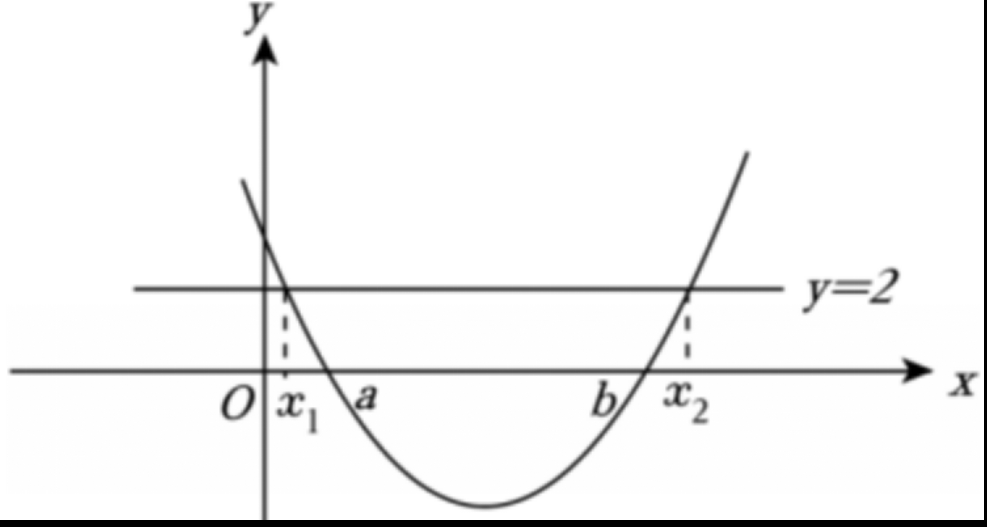
\includegraphics[width=0.42\textwidth]{figures/gao100_q16_parabola.png}
\end{center}
\step{所以数形结合得 $x_1<a<b<x_2$．故选 $B$.}
\solend
\fi

\end{enumerate}

\bigsec{三、解答题}

\begin{enumerate}
\setcounter{enumi}{16}

\item 已知集合 $A=\{x\mid3<x\leqslant6\}$，$B=\{x\mid m\leqslant x\leqslant2m+1\}$.

（1）若 $m=2$，求 $A\cap B$、$A\cup B$；

（2）若 $x\in B$ 是 $x\in A$ 的必要条件，求实数 $m$ 的取值范围.

\ansspace*[9]

\ifanswer
\solbegin
\stepm{（1）}{若 $m=2$，则 $B=\{x\mid2\leqslant x\leqslant5\}$，因为 $A=\{x\mid3<x\leqslant6\}$，}
\step{所以 $A\cap B=\{x\mid3<x\leqslant5\}$，$A\cup B=\{x\mid2\leqslant x\leqslant6\}$.}
\stepm{（2）}{因为 $x\in B$ 是 $x\in A$ 的必要条件，所以 $A\subseteq B$，}
\step{所以 $\begin{cases}m\leqslant3\\ 2m+1\geqslant6\end{cases}$，所以 $\dfrac52\leqslant m\leqslant3$，所以实数 $m$ 的取值范围为 $\left[\dfrac52,3\right]$.}
\solend
\fi

\item 求关于 $x$ 的不等式 $3ax^2-(3a+2)x+2<0\,(a\in R)$ 的解集.

\ansspace*[10]

\ifanswer
\solbegin
\step{当 $a=0$ 时，不等式化为 $-2x+2<0$，解得 $x>1$，}
\step{当 $a\neq0$ 时，方程 $3ax^2-(3a+2)x+2=0$ 的两根分别为 $1$，$\dfrac2{3a}$}
\step{当 $\dfrac2{3a}=1$，即 $a=\dfrac23$ 时，不等式化为 $(x-1)^2<0$，不等式无解，}
\step{当 $\dfrac2{3a}<1$，即 $a>\dfrac23$ 时，不等式解集为 $\left(\dfrac2{3a},1\right)$，}
\step{当 $0<a<\dfrac23$ 时，$\dfrac2{3a}>1$，不等式的解集为 $\left(1,\dfrac2{3a}\right)$，}
\step{当 $a<0$ 时，不等式的解集为 $\left(-\infty,\dfrac2{3a}\right)\cup(1,+\infty)$，}
\step{综上，当 $a=0$ 时，不等式的解集为 $(1,+\infty)$，}
\step{当 $a=\dfrac23$ 时，不等式的解集为 $\varnothing$，}
\step{当 $a>\dfrac23$ 时，不等式解集为 $\left(\dfrac2{3a},1\right)$，}
\step{当 $0<a<\dfrac23$ 时，不等式的解集为 $\left(1,\dfrac2{3a}\right)$，}
\step{当 $a<0$ 时，不等式的解集为 $\left(-\infty,\dfrac2{3a}\right)\cup(1,+\infty)$.}
\solend
\fi

\item 设对于任意实数 $x$，不等式 $\lvert x+1\rvert+\lvert x-1\rvert\geqslant m$ 恒成立.

（1）求 $m$ 的取值范围；

（2）当 $m$ 取最大值时，解关于 $x$ 的不等式 $\lvert x-3\rvert-2x\leqslant2m-2$.

\ansspace*[9]

\ifanswer
\solbegin
\stepm{（1）}{设函数 $f(x)=\lvert x+1\rvert+\lvert x-1\rvert$，则 $f(x)=\begin{cases}-2x,&x\leqslant-1\\ 2,&-1<x<1\\ 2x,&x\geqslant1\end{cases}$，}
\step{当 $x\leqslant-1$ 时，$f(x)$ 有最小值 2；}
\step{当 $-1<x<1$ 时，$f(x)=2$；}
\step{当 $x\geqslant1$ 时，$f(x)$ 有最小值 2；}
\step{因为对于任意实数 $x$，不等式 $\lvert x+1\rvert+\lvert x-1\rvert\geqslant m$ 恒成立，}
\step{所以 $m\leqslant2$，即 $m$ 的取值范围为 $(-\infty,2]$；}
\stepm{（2）}{由（1）得 $m$ 的最大值为 2，所以原不等式为 $\lvert x-3\rvert\leqslant2x+2$，}
\step{即 $-2x-2\leqslant x-3\leqslant2x+2$，解得 $x\geqslant\dfrac13$，}
\step{所以原不等式的解集为 $\left\{x\mid x\geqslant\dfrac13\right\}$.}
\solend
\fi

\item 某轮船公司的一艘轮船每小时花费的燃料费与轮船航行速度的平方成正比，比例系数为 $k$．轮船的最大速度为 18 海里/小时．当船速为 10 海里/小时，它的燃料费是每小时 120 元，其余航行运作费用（不论速度如何）总计是每小时 120 元．假定运行过程中轮船以速度 $v$ 匀速航行.

（1）求 $k$ 的值及每小时的最大总费用 $H$；

（2）求该轮船航行 100 海里的总费用 $W$（燃料费＋其余航行运作费用）的最小值.

\ansspace*[10]

\ifanswer
\solbegin
\stepm{（1）}{由题意，每小时燃料费为 $h(v)=kv^2$，$0<v\leqslant18$，}
\step{已知 $v=10$ 时，燃料费每小时 120 元，则 $k\cdot10^2=120$，得 $k=1.2$，}
\step{每小时总费用 $h(v)=kv^2+120=1.2v^2+120$，}
\step{$h(v)$ 是关于 $v$ 的增函数，$v$ 最大为 18，}
\step{所以 $H=h(18)=1.2\times18^2+120=508.8$ 元.}
\stepm{（2）}{航行时间 $t=\dfrac{100}v$ 小时，}
\step{$W(v)=h(v)\cdot t=(1.2v^2+120)\cdot\dfrac{100}v,0<v\leqslant18=120v+\dfrac{12000}v$，}
\step{利用均值不等式 $120v+\dfrac{12000}v\geqslant2\sqrt{120v\cdot\dfrac{12000}v}=2\times1200=2400$，}
\step{当且仅当 $120v=\dfrac{12000}v$，即 $v=10$ 时取等号，}
\step{$v=10\leqslant18$，在速度范围内，可取到等号，所以总费用最小值为 2400 元.}
\solend
\fi

\item 已知 $A$ 是 $R$ 的非空真子集，如果对任意 $x$、$y\in A$，都有 $x+y\in A$，$xy\in A$，则称 $A$ 是封闭集.

（1）判断集合 $B=\{0\}$，$C=\{-1,0,1\}$ 是否为封闭集，并说明理由；

（2）判断以下两个命题的真假，并说明理由；

命题 $p$：若非空集合 $A_1$、$A_2$ 是封闭集，则 $A_1\cup A_2$ 也是封闭集；

命题 $q$：非空集合 $A_1$、$A_2$ 是封闭集，则 $A_1\cap A_2\neq\varnothing$ 是 $A_1\cap A_2$ 是封闭集的充要条件；

（3）若非空集合 $A$ 是封闭集合，设全集为 $R$，求证：$A$ 的补集不是封闭集.

\ansspace*[13]

\ifanswer
\solbegin
\stepm{（1）}{$B=\{0\}$ 是封闭集，$C=\{-1,0,1\}$ 不是封闭集，理由如下：}
\step{对于集合 $B=\{0\}$，因为 $0+0=0\in B$，$0\times0=0\in B$，}
\step{所以 $B=\{0\}$ 是封闭集；}
\step{对于集合 $C=\{-1,0,1\}$，因为 $-1+(-1)=-2\notin C$，$1+1=2\notin C$，}
\step{所以集合 $C=\{-1,0,1\}$ 不是封闭集.}
\stepm{（2）}{命题 $p$ 是假命题，命题 $q$ 是真命题，理由如下：}
\step{对命题 $p$：令 $A_1=\{x\mid x=2k,k\in Z\}$，$A_2=\{x\mid x=3k,k\in Z\}$，}
\step{令 $x_1=2k_1$，$y_1=2k_2$，$k_1$、$k_2\in Z$，}
\step{则 $x_1+y_1=2(k_1+k_2)\in A_1$，$x_1y_1=2(2k_1k_2)\in A_1$，}
\step{因此集合 $A_1$ 是封闭集，同理集合 $A_2$ 也是封闭集，}
\step{取 $x_2=2$，$y_2=3$，则 $x_2$、$y_2\in(A_1\cup A_2)$，而 $x_2+y_2=5\notin(A_1\cup A_2)$，}
\step{因此集合 $A_1\cup A_2$ 不是封闭集，命题 $p$ 是假命题；}
\step{对于命题 $q$：若 $A_1\cap A_2\neq\varnothing$，不妨令 $a$、$b\in(A_1\cap A_2)$，}
\step{则有 $a$、$b\in A_1$，又集合 $A_1$ 是封闭集，则 $a+b\in A_1$，$ab\in A_1$，}
\step{同理 $a+b\in A_2$，$ab\in A_2$，因此 $a+b\in(A_1\cap A_2)$，$ab\in(A_1\cap A_2)$，}
\step{所以 $A_1\cap A_2$ 是封闭集；}
\step{反之，若 $A_1\cap A_2$ 是封闭集，则 $A_1\cap A_2$ 是非空集合，即 $A_1\cap A_2\neq\varnothing$，}
\step{所以 $A_1\cap A_2$ 是 $A_1\cap A_2$ 是封闭集的充要条件，命题 $q$ 是真命题.}
\stepm{（3）}{非空集合 $A$ 是封闭集合，当 $A=R$ 时，$\overline A=\varnothing$，因此 $\overline A$ 不是封闭集合；}
\step{当 $A\neq R$ 时，假设 $\overline A$ 是封闭集合，}
\step{设 $0\in A$，在 $\overline A$ 中任取一个 $x$，$x\neq0$，则 $-x\in A$，}
\step{否则 $-x\in\overline A$，此时 $x+(-x)=0\in\overline A$，与 $0\in A$ 矛盾，}
\step{因此 $(-x)^2\in A$，$x^2\in\overline A$，而 $(-x)^2=x^2$，与 $A\cap\overline A=\varnothing$ 矛盾，}
\step{则当 $0\in A$ 时，则 $\overline A$ 不是封闭集合，同理当 $0\in\overline A$ 时，$\overline A$ 不是封闭集合，}
\step{所以 $A$ 的补集不是封闭集.}
\solend
\fi

\end{enumerate}

\end{document}
"
% 紧凑版：xelatex "\def\iscompact{1}% 高一100_南洋中学_10月月考.tex
%   —— 高一上数学“2026-2027 年南洋中学高一上 10 月月考”（讲评版）
% 试卷版：xelatex 高一100_南洋中学_10月月考.tex
% 答案版：xelatex "\def\isanswer{1}% 高一100_南洋中学_10月月考.tex
%   —— 高一上数学“2026-2027 年南洋中学高一上 10 月月考”（讲评版）
% 试卷版：xelatex 高一100_南洋中学_10月月考.tex
% 答案版：xelatex "\def\isanswer{1}\input{高一100_南洋中学_10月月考.tex}"
% 紧凑版：xelatex "\def\iscompact{1}\input{高一100_南洋中学_10月月考.tex}"
%
% 原始材料：微信公众号“魔都数学加油站”文章，连载“27学年高一100”；
% 原文标题“27学年高一100——2026-2027年上海市南洋中学高一上10月月考”；
% 原文链接：https://mp.weixin.qq.com/s/uXLyt6VHraW4hSpDwnZDuQ。
% 正文为 10 张 PNG 页（`原图/高一100_南洋中学_10月月考/01..10.png`），
% 尺寸混排（第 2、4—9 页为 4762×6735，第 1、3、10 页为 2560×3620），按页序读取。
%
% 篇幅与题号：原卷自第 3 题起编号（第 1、2 题不在原文内）。填空题 3—12（10 题）、
% 选择题 13—16（4 题）、解答题 17—21（5 题），共 19 题。
%
% 讲评版：全部 19 题均印【解析】，其中第 13—16 题的答案在解析末句
% “故选 $C$／$B$／$D$／$B$”（题干括号内未印答案）。第 16 题解析带一幅
% 抛物线与 $y=2$ 的示意图，自原图裁切、去粉色水印后转灰度，三版都出。
%
% 副标题：原卷未印副标题。本稿按内容标作“集合与常用逻辑用语、不等式”。
%
% 原卷笔误/存疑（均照录未改，正文对应处另有 % 注）：无。
%
% 与原卷的排版差异：
%   ① 原卷每题下直接印【解析】，本稿按全稿惯例将答案与解析置于答案版；
%   ② 原卷未印副标题，本稿补出；填空横线统一排 \blankline[4.4em]；
%   ③ 原卷数集记号排斜体 $R$、$Z$、$\mathit N$，本稿按全稿惯例改用 $\R$、$\Z$、$\N$；
%   ④ 解答题按惯例加 \ansspace；选择题括号排 \mbox{（\quad）}；
%   ⑤ 第 16 题的示意图原卷排在解析行右侧，本稿改排为解析后的居中图。
%
% 行数核对：逐题数 \step/\stepm 条数，合计 117 条（Q3：2；Q4：5；Q5：7；Q6：3；Q7：3；
% Q8：4；Q9：2；Q10：4；Q11：6；Q12：3；Q13：7；Q14：3；Q15：5；Q16：3；Q17：5；
% Q18：11；Q19：9；Q20：10；Q21：25）。全卷 19 题均印【解析】。
% 原卷解析的换行按语意合并，未逐行强拆。
%
\documentclass[a4paper,11pt]{article}
\usepackage{common}
\begin{document}

\examtitlest[7]{2026--2027 年南洋中学高一上 10 月月考}{集合与常用逻辑用语、不等式}

\bigsec{一、填空题}

\begin{enumerate}
\setcounter{enumi}{2}

\item 不等式 $\dfrac{x-6}{x+1}\geqslant0$ 的解集为\blankline[4.4em].

\ifanswer
\solbegin
\step{不等式 $\dfrac{x-6}{x+1}\geqslant0$ 等价于 $\begin{cases}(x-6)(x+1)\geqslant0\\ x+1\neq0\end{cases}$，即 $x<-1$ 或 $x\geqslant6$，}
\step{故解集为 $(-\infty,-1)\cup[6,+\infty)$.}
\solend
\fi

\item 已知关于 $x$ 的不等式 $ax^2+bx+c>0$ 的解集是 $(1,3)$，则关于 $x$ 的不等式 $ax^2-bx+c\leqslant0$ 的解集为\blankline[4.4em].

\ifanswer
\solbegin
\step{由已知得 $a<0$，且 $1$，$3$ 是方程 $ax^2+bx+c=0$ 的根，}
\step{所以 $\begin{cases}1+3=-\dfrac ba\\[2pt] 1\times3=\dfrac ca\end{cases}$，所以 $\begin{cases}b=-4a\\ c=3a\end{cases}$，}
\step{所以 $ax^2-bx+c\leqslant0$ 可变形为 $ax^2+4ax+3a\leqslant0$，}
\step{因为 $a<0$，所以 $x^2+4x+3\geqslant0$，解得 $x\leqslant-3$ 或 $x\geqslant-1$，}
\step{所以不等式的解集为 $(-\infty,-3]\cup[-1,+\infty)$.}
\solend
\fi

\item 不等式 $\lvert x+2\rvert+\lvert 2x-1\rvert\geqslant3$ 的解集为\blankline[4.4em].

\ifanswer
\solbegin
\step{当 $x\leqslant-2$ 时，$x+2\leqslant0$，$2x-1<0$，}
\step{所以 $\lvert x+2\rvert+\lvert 2x-1\rvert=-x-2-2x+1\geqslant3$，解得 $x\leqslant-\dfrac43$；}
\step{当 $-2<x<\dfrac12$ 时，$x+2>0$，$2x-1<0$，}
\step{所以 $\lvert x+2\rvert+\lvert 2x-1\rvert=x+2-2x+1\geqslant3$，解得 $x\leqslant0$；}
\step{当 $x\geqslant\dfrac12$ 时，$x+2>0$，$2x-1\geqslant0$，}
\step{所以 $\lvert x+2\rvert+\lvert 2x-1\rvert=x+2+2x-1\geqslant3$，解得 $x\geqslant\dfrac23$；}
\step{所以原不等式的解集为 $\left\{x\mid x\leqslant0\right.$ 或 $\left.x\geqslant\dfrac23\right\}$.}
\solend
\fi

\item 若正数 $x$、$y$ 满足 $x+2y=2$，则 $\dfrac1x+\dfrac2y$ 的最小值是\blankline[4.4em].

\ifanswer
\solbegin
\step{因为 $x>0$，$y>0$，且 $x+2y=2$，}
\step{所以 $\dfrac1x+\dfrac2y=\dfrac12\left(\dfrac1x+\dfrac2y\right)(x+2y)=\dfrac12\left(5+\dfrac{2y}x+\dfrac{2x}y\right)\geqslant\dfrac12\left(5+2\sqrt{\dfrac{2y}x\cdot\dfrac{2x}y}\right)=\dfrac92$.}
\step{当且仅当 $\begin{cases}x+2y=2\\ \dfrac{2y}x=\dfrac{2x}y\end{cases}$，即 $x=y=\dfrac23$ 时取等号，故最小值为 $\dfrac92$.}
\solend
\fi

\item 已知 $\alpha:x\leqslant2$ 或 $x>3$，$\beta:x\leqslant m+5$ 或 $x>-m$，若 $\alpha$ 是 $\beta$ 的必要非充分条件，则实数 $m$ 的取值范围是\blankline[4.4em].

\ifanswer
\solbegin
\step{设 $A=\{x\mid x\leqslant2$ 或 $x>3\}$，$B=\{x\mid x\leqslant m+5$ 或 $x>-m\}$，则 $B\subset A$，}
\step{则 $m+5\leqslant2$ 且 $-m\geqslant3$（等号不能同时取得），则 $m<-3$，}
\step{则实数 $m$ 的取值范围是 $(-\infty,-3)$.}
\solend
\fi

\item 已知集合 $A=\{x\mid-1\leqslant x\leqslant3\}$，$B=\{x\mid ax+1>0\}$ 满足 $A\subseteq B$，则实数 $a$ 的取值范围为\blankline[4.4em].

\ifanswer
\solbegin
\step{当 $a=0$ 时，$B=R$，显然符合题意，}
\step{当 $a>0$ 时，$B=\left\{x\mid x>-\dfrac1a\right\}$，则 $-\dfrac1a<-1$，解得 $a<1$，所以 $0<a<1$，}
\step{当 $a<0$ 时，$B=\left\{x\mid x<-\dfrac1a\right\}$，则 $-\dfrac1a>3$，解得 $a>-\dfrac13$，所以 $-\dfrac13<a<0$，}
\step{综上所述，实数 $a$ 的取值范围为 $\left(-\dfrac13,1\right)$.}
\solend
\fi

\item 设集合 $A=\{x\mid3x-1<m\}$，若 $1\in A$ 且 $2\notin A$，则实数 $m$ 的取值范围是\blankline[4.4em].

\ifanswer
\solbegin
\step{因为集合 $A=\{x\mid3x-1<m\}$，若 $1\in A$ 且 $2\notin A$，}
\step{则 $3\times1-1<m$ 且 $3\times2-1\geqslant m$，解得 $2<m\leqslant5$.}
\solend
\fi

\item 若 $M=\left\{x\mid x=m+\dfrac16,m\in Z\right\},N=\left\{x\mid x=\dfrac n2-\dfrac13,n\in Z\right\}$，\newline $P=\left\{x\mid x=\dfrac p2+\dfrac16,p\in Z\right\}$，则 $M$、$N$、$P$ 的关系为\blankline[4.4em].

\ifanswer
\solbegin
\step{$M=\left\{x\mid x=m+\dfrac16=\dfrac{6m+1}6=\dfrac{3\cdot2m+1}6,m\in Z\right\}$，}
\step{$N=\left\{x\mid x=\dfrac n2-\dfrac13=\dfrac{3(n-1)+1}6,n\in Z\right\}=\left\{x\mid x=\dfrac{3k+1}6,k\in Z\right\}$，}
\step{$P=\left\{x\mid x=\dfrac p2+\dfrac16=\dfrac{3p+1}6,p\in Z\right\}$，}
\step{故 $M\subset N=P$.}
\solend
\fi

\item 已知命题 $p:x<-2$ 或 $x>3$，命题 $q:x<3m+1$ 或 $x>m+2$，若 $p$ 是 $q$ 的充分非必要条件，则实数 $m$ 的取值范围是\blankline[4.4em].

\ifanswer
\solbegin
\step{设 $A=\{x\mid x<-2$ 或 $x>3\}$，$B=\{x\mid x<3m+1$ 或 $x>m+2\}$，}
\step{若 $p$ 是 $q$ 的充分非必要条件，则 $A\subset B$，}
\step{当 $3m+1\geqslant m+2$，即 $m\geqslant\dfrac12$ 时，显然有 $A\subset B$，}
\step{当 $3m+1<m+2$，即 $m<\dfrac12$ 时，}
\step{由 $A\subset B$，则 $\begin{cases}m+2\leqslant3\\ 3m+1\geqslant-2\end{cases}$（等号不同时成立），即 $-1\leqslant m<\dfrac12$.}
\step{综上，实数 $m$ 的取值范围是 $[-1,+\infty)$.}
\solend
\fi

\item 对于一个有限集 $A$，一般都可以找到两个非空数集 $A_1$ 和 $A_2$，满足 $A_1\cap A_2=\varnothing$，且 $A_1\cup A_2=A$，记集合 $\{A_1,A_2\}$ 为 $A$ 的一个“划分集”．若 $A$ 中有 $n(n\geqslant2,n\in\N)$ 个元素，则不同的“划分集”共有\blankline[4.4em]个(用含 $n$ 的表达式填空).

\ifanswer
\solbegin
\step{集合中的每个元素都有属于 $A_1$ 或属于 $A_2$ 两种情况，故共有 $2^n$ 种情况，}
\step{排除全都属于 $A_1$ 或 $A_2$ 的两种情况，考虑对称情况，}
\step{故不同的“划分集”共有 $\dfrac12(2^n-2)=2^{n-1}-1$ 个.}
\solend
\fi

\end{enumerate}

\bigsec{二、选择题}

\begin{enumerate}
\setcounter{enumi}{12}

\item 下列命题中正确的\mbox{（\quad）}

\keepwithprev
A. $\varnothing$ 与 $\{0\}$ 表示同一个集合

B. 方程 $\{x\mid(x-2)^2(x-3)=0\}$ 的所有解的集合可表示为 $\{2,2,3\}$

C. 由 3，4，5 组成的集合可表示为 $\{3,4,5\}$ 或 $\{4,5,3\}$

D. 很小的实数可以构成集合.

\ifanswer
\solbegin
\step{对于 $A$，$\{0\}$ 中有一个元素 0，$\varnothing$ 中无任何元素，故 $\varnothing$ 与 $\{0\}$ 不是同一个集合，}
\step{故 $A$ 错误；}
\step{对于 $B$，$\{2,2,3\}$ 不满足集合元素的互异性，故 $B$ 错误；}
\step{对于 $C$，由集合的无序性，得由 3，4，5 组成的集合可表示为 $\{3,4,5\}$ 或 $\{4,5,3\}$，}
\step{故 $C$ 正确；}
\step{对于 $D$，由集合的确定性，很小的实数不能构成集合，故 $D$ 错误.}
\step{故选 $C$.}
\solend
\fi

\item 已知 $a\in R$，则“$\dfrac1a<1$”是“$a>1$”的\mbox{（\quad）}条件.

\keepwithprev
A. 充分非必要\qquad B. 必要非充分

C. 充要\qquad D. 既非充分又非必要

\ifanswer
\solbegin
\step{解 $\dfrac1a<1$，得 $a<0$ 或 $a>1$，}
\step{由 $a<0$ 或 $a>1$ 得不出 $a>1$，由 $a>1$ 得出 $a<0$ 或 $a>1$，}
\step{所以“$\dfrac1a<1$”是“$a>1$”的必要不充分条件．故选 $B$.}
\solend
\fi

\item 若命题“存在 $x_0\in R$ 使得 $ax_0^2+2ax_0+1\leqslant0$”是假命题，则实数 $a$ 的取值范围为\mbox{（\quad）}

\keepwithprev
A. $a<0$ 或 $a\geqslant1$\qquad B. $a\leqslant0$ 或 $a\geqslant1$\qquad C. $0<a<1$\qquad D. $0\leqslant a<1$

\ifanswer
\solbegin
\step{命题“存在 $x_0\in R$ 使得 $ax_0^2+2ax_0+1\leqslant0$”是假命题，}
\step{则 $\forall x\in R$，$ax^2+2ax+1>0$ 恒成立，}
\step{当 $a=0$ 时，满足题意，}
\step{当 $a\neq0$ 时，$\begin{cases}a>0\\ \Delta=4a^2-4a<0\end{cases}$，解得 $0<a<1$，}
\step{综上所述，实数 $a$ 的取值范围为 $\{a\mid0\leqslant a<1\}$．故选 $D$.}
\solend
\fi

\item 已知实数 $a<b$，关于 $x$ 的不等式 $x^2-(a+b)x+ab-2<0$ 的解集为 $(x_1,x_2)$，则实数 $a$、$b$、$x_1$、$x_2$ 从小到大的排列是\mbox{（\quad）}

\keepwithprev
A. $a<x_1<x_2<b$\qquad B. $x_1<a<b<x_2$\qquad C. $a<x_1<b<x_2$\qquad D. $x_1<a<x_2<b$

\ifanswer
\solbegin
\step{因为实数 $a<b$，不等式 $x^2-(a+b)x+ab-2<0$ 可化为 $(x-a)(x-b)<2$，}
\step{又其解集为 $(x_1,x_2)$，所以作出 $y=(x-a)(x-b)$ 与 $y=2$ 的图象如下：}
\begin{center}
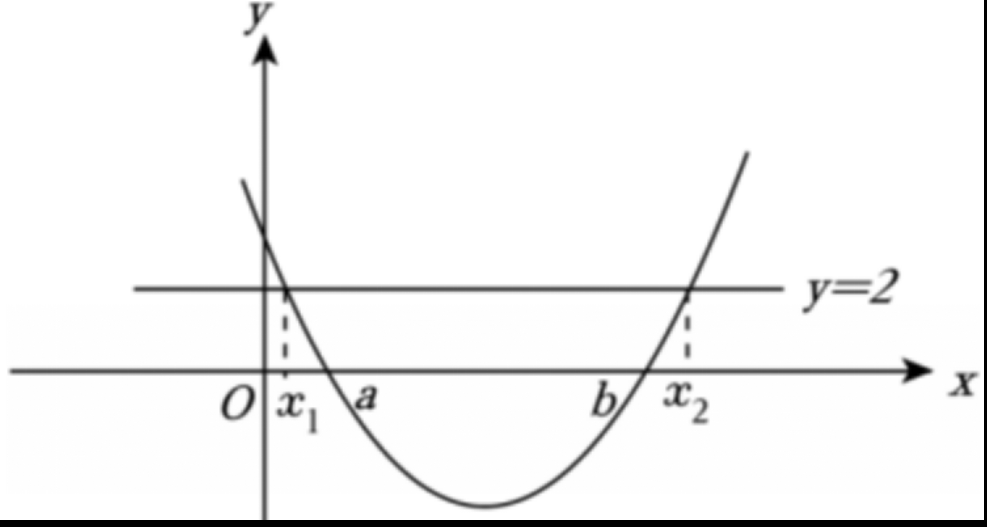
\includegraphics[width=0.42\textwidth]{figures/gao100_q16_parabola.png}
\end{center}
\step{所以数形结合得 $x_1<a<b<x_2$．故选 $B$.}
\solend
\fi

\end{enumerate}

\bigsec{三、解答题}

\begin{enumerate}
\setcounter{enumi}{16}

\item 已知集合 $A=\{x\mid3<x\leqslant6\}$，$B=\{x\mid m\leqslant x\leqslant2m+1\}$.

（1）若 $m=2$，求 $A\cap B$、$A\cup B$；

（2）若 $x\in B$ 是 $x\in A$ 的必要条件，求实数 $m$ 的取值范围.

\ansspace*[9]

\ifanswer
\solbegin
\stepm{（1）}{若 $m=2$，则 $B=\{x\mid2\leqslant x\leqslant5\}$，因为 $A=\{x\mid3<x\leqslant6\}$，}
\step{所以 $A\cap B=\{x\mid3<x\leqslant5\}$，$A\cup B=\{x\mid2\leqslant x\leqslant6\}$.}
\stepm{（2）}{因为 $x\in B$ 是 $x\in A$ 的必要条件，所以 $A\subseteq B$，}
\step{所以 $\begin{cases}m\leqslant3\\ 2m+1\geqslant6\end{cases}$，所以 $\dfrac52\leqslant m\leqslant3$，所以实数 $m$ 的取值范围为 $\left[\dfrac52,3\right]$.}
\solend
\fi

\item 求关于 $x$ 的不等式 $3ax^2-(3a+2)x+2<0\,(a\in R)$ 的解集.

\ansspace*[10]

\ifanswer
\solbegin
\step{当 $a=0$ 时，不等式化为 $-2x+2<0$，解得 $x>1$，}
\step{当 $a\neq0$ 时，方程 $3ax^2-(3a+2)x+2=0$ 的两根分别为 $1$，$\dfrac2{3a}$}
\step{当 $\dfrac2{3a}=1$，即 $a=\dfrac23$ 时，不等式化为 $(x-1)^2<0$，不等式无解，}
\step{当 $\dfrac2{3a}<1$，即 $a>\dfrac23$ 时，不等式解集为 $\left(\dfrac2{3a},1\right)$，}
\step{当 $0<a<\dfrac23$ 时，$\dfrac2{3a}>1$，不等式的解集为 $\left(1,\dfrac2{3a}\right)$，}
\step{当 $a<0$ 时，不等式的解集为 $\left(-\infty,\dfrac2{3a}\right)\cup(1,+\infty)$，}
\step{综上，当 $a=0$ 时，不等式的解集为 $(1,+\infty)$，}
\step{当 $a=\dfrac23$ 时，不等式的解集为 $\varnothing$，}
\step{当 $a>\dfrac23$ 时，不等式解集为 $\left(\dfrac2{3a},1\right)$，}
\step{当 $0<a<\dfrac23$ 时，不等式的解集为 $\left(1,\dfrac2{3a}\right)$，}
\step{当 $a<0$ 时，不等式的解集为 $\left(-\infty,\dfrac2{3a}\right)\cup(1,+\infty)$.}
\solend
\fi

\item 设对于任意实数 $x$，不等式 $\lvert x+1\rvert+\lvert x-1\rvert\geqslant m$ 恒成立.

（1）求 $m$ 的取值范围；

（2）当 $m$ 取最大值时，解关于 $x$ 的不等式 $\lvert x-3\rvert-2x\leqslant2m-2$.

\ansspace*[9]

\ifanswer
\solbegin
\stepm{（1）}{设函数 $f(x)=\lvert x+1\rvert+\lvert x-1\rvert$，则 $f(x)=\begin{cases}-2x,&x\leqslant-1\\ 2,&-1<x<1\\ 2x,&x\geqslant1\end{cases}$，}
\step{当 $x\leqslant-1$ 时，$f(x)$ 有最小值 2；}
\step{当 $-1<x<1$ 时，$f(x)=2$；}
\step{当 $x\geqslant1$ 时，$f(x)$ 有最小值 2；}
\step{因为对于任意实数 $x$，不等式 $\lvert x+1\rvert+\lvert x-1\rvert\geqslant m$ 恒成立，}
\step{所以 $m\leqslant2$，即 $m$ 的取值范围为 $(-\infty,2]$；}
\stepm{（2）}{由（1）得 $m$ 的最大值为 2，所以原不等式为 $\lvert x-3\rvert\leqslant2x+2$，}
\step{即 $-2x-2\leqslant x-3\leqslant2x+2$，解得 $x\geqslant\dfrac13$，}
\step{所以原不等式的解集为 $\left\{x\mid x\geqslant\dfrac13\right\}$.}
\solend
\fi

\item 某轮船公司的一艘轮船每小时花费的燃料费与轮船航行速度的平方成正比，比例系数为 $k$．轮船的最大速度为 18 海里/小时．当船速为 10 海里/小时，它的燃料费是每小时 120 元，其余航行运作费用（不论速度如何）总计是每小时 120 元．假定运行过程中轮船以速度 $v$ 匀速航行.

（1）求 $k$ 的值及每小时的最大总费用 $H$；

（2）求该轮船航行 100 海里的总费用 $W$（燃料费＋其余航行运作费用）的最小值.

\ansspace*[10]

\ifanswer
\solbegin
\stepm{（1）}{由题意，每小时燃料费为 $h(v)=kv^2$，$0<v\leqslant18$，}
\step{已知 $v=10$ 时，燃料费每小时 120 元，则 $k\cdot10^2=120$，得 $k=1.2$，}
\step{每小时总费用 $h(v)=kv^2+120=1.2v^2+120$，}
\step{$h(v)$ 是关于 $v$ 的增函数，$v$ 最大为 18，}
\step{所以 $H=h(18)=1.2\times18^2+120=508.8$ 元.}
\stepm{（2）}{航行时间 $t=\dfrac{100}v$ 小时，}
\step{$W(v)=h(v)\cdot t=(1.2v^2+120)\cdot\dfrac{100}v,0<v\leqslant18=120v+\dfrac{12000}v$，}
\step{利用均值不等式 $120v+\dfrac{12000}v\geqslant2\sqrt{120v\cdot\dfrac{12000}v}=2\times1200=2400$，}
\step{当且仅当 $120v=\dfrac{12000}v$，即 $v=10$ 时取等号，}
\step{$v=10\leqslant18$，在速度范围内，可取到等号，所以总费用最小值为 2400 元.}
\solend
\fi

\item 已知 $A$ 是 $R$ 的非空真子集，如果对任意 $x$、$y\in A$，都有 $x+y\in A$，$xy\in A$，则称 $A$ 是封闭集.

（1）判断集合 $B=\{0\}$，$C=\{-1,0,1\}$ 是否为封闭集，并说明理由；

（2）判断以下两个命题的真假，并说明理由；

命题 $p$：若非空集合 $A_1$、$A_2$ 是封闭集，则 $A_1\cup A_2$ 也是封闭集；

命题 $q$：非空集合 $A_1$、$A_2$ 是封闭集，则 $A_1\cap A_2\neq\varnothing$ 是 $A_1\cap A_2$ 是封闭集的充要条件；

（3）若非空集合 $A$ 是封闭集合，设全集为 $R$，求证：$A$ 的补集不是封闭集.

\ansspace*[13]

\ifanswer
\solbegin
\stepm{（1）}{$B=\{0\}$ 是封闭集，$C=\{-1,0,1\}$ 不是封闭集，理由如下：}
\step{对于集合 $B=\{0\}$，因为 $0+0=0\in B$，$0\times0=0\in B$，}
\step{所以 $B=\{0\}$ 是封闭集；}
\step{对于集合 $C=\{-1,0,1\}$，因为 $-1+(-1)=-2\notin C$，$1+1=2\notin C$，}
\step{所以集合 $C=\{-1,0,1\}$ 不是封闭集.}
\stepm{（2）}{命题 $p$ 是假命题，命题 $q$ 是真命题，理由如下：}
\step{对命题 $p$：令 $A_1=\{x\mid x=2k,k\in Z\}$，$A_2=\{x\mid x=3k,k\in Z\}$，}
\step{令 $x_1=2k_1$，$y_1=2k_2$，$k_1$、$k_2\in Z$，}
\step{则 $x_1+y_1=2(k_1+k_2)\in A_1$，$x_1y_1=2(2k_1k_2)\in A_1$，}
\step{因此集合 $A_1$ 是封闭集，同理集合 $A_2$ 也是封闭集，}
\step{取 $x_2=2$，$y_2=3$，则 $x_2$、$y_2\in(A_1\cup A_2)$，而 $x_2+y_2=5\notin(A_1\cup A_2)$，}
\step{因此集合 $A_1\cup A_2$ 不是封闭集，命题 $p$ 是假命题；}
\step{对于命题 $q$：若 $A_1\cap A_2\neq\varnothing$，不妨令 $a$、$b\in(A_1\cap A_2)$，}
\step{则有 $a$、$b\in A_1$，又集合 $A_1$ 是封闭集，则 $a+b\in A_1$，$ab\in A_1$，}
\step{同理 $a+b\in A_2$，$ab\in A_2$，因此 $a+b\in(A_1\cap A_2)$，$ab\in(A_1\cap A_2)$，}
\step{所以 $A_1\cap A_2$ 是封闭集；}
\step{反之，若 $A_1\cap A_2$ 是封闭集，则 $A_1\cap A_2$ 是非空集合，即 $A_1\cap A_2\neq\varnothing$，}
\step{所以 $A_1\cap A_2$ 是 $A_1\cap A_2$ 是封闭集的充要条件，命题 $q$ 是真命题.}
\stepm{（3）}{非空集合 $A$ 是封闭集合，当 $A=R$ 时，$\overline A=\varnothing$，因此 $\overline A$ 不是封闭集合；}
\step{当 $A\neq R$ 时，假设 $\overline A$ 是封闭集合，}
\step{设 $0\in A$，在 $\overline A$ 中任取一个 $x$，$x\neq0$，则 $-x\in A$，}
\step{否则 $-x\in\overline A$，此时 $x+(-x)=0\in\overline A$，与 $0\in A$ 矛盾，}
\step{因此 $(-x)^2\in A$，$x^2\in\overline A$，而 $(-x)^2=x^2$，与 $A\cap\overline A=\varnothing$ 矛盾，}
\step{则当 $0\in A$ 时，则 $\overline A$ 不是封闭集合，同理当 $0\in\overline A$ 时，$\overline A$ 不是封闭集合，}
\step{所以 $A$ 的补集不是封闭集.}
\solend
\fi

\end{enumerate}

\end{document}
"
% 紧凑版：xelatex "\def\iscompact{1}% 高一100_南洋中学_10月月考.tex
%   —— 高一上数学“2026-2027 年南洋中学高一上 10 月月考”（讲评版）
% 试卷版：xelatex 高一100_南洋中学_10月月考.tex
% 答案版：xelatex "\def\isanswer{1}\input{高一100_南洋中学_10月月考.tex}"
% 紧凑版：xelatex "\def\iscompact{1}\input{高一100_南洋中学_10月月考.tex}"
%
% 原始材料：微信公众号“魔都数学加油站”文章，连载“27学年高一100”；
% 原文标题“27学年高一100——2026-2027年上海市南洋中学高一上10月月考”；
% 原文链接：https://mp.weixin.qq.com/s/uXLyt6VHraW4hSpDwnZDuQ。
% 正文为 10 张 PNG 页（`原图/高一100_南洋中学_10月月考/01..10.png`），
% 尺寸混排（第 2、4—9 页为 4762×6735，第 1、3、10 页为 2560×3620），按页序读取。
%
% 篇幅与题号：原卷自第 3 题起编号（第 1、2 题不在原文内）。填空题 3—12（10 题）、
% 选择题 13—16（4 题）、解答题 17—21（5 题），共 19 题。
%
% 讲评版：全部 19 题均印【解析】，其中第 13—16 题的答案在解析末句
% “故选 $C$／$B$／$D$／$B$”（题干括号内未印答案）。第 16 题解析带一幅
% 抛物线与 $y=2$ 的示意图，自原图裁切、去粉色水印后转灰度，三版都出。
%
% 副标题：原卷未印副标题。本稿按内容标作“集合与常用逻辑用语、不等式”。
%
% 原卷笔误/存疑（均照录未改，正文对应处另有 % 注）：无。
%
% 与原卷的排版差异：
%   ① 原卷每题下直接印【解析】，本稿按全稿惯例将答案与解析置于答案版；
%   ② 原卷未印副标题，本稿补出；填空横线统一排 \blankline[4.4em]；
%   ③ 原卷数集记号排斜体 $R$、$Z$、$\mathit N$，本稿按全稿惯例改用 $\R$、$\Z$、$\N$；
%   ④ 解答题按惯例加 \ansspace；选择题括号排 \mbox{（\quad）}；
%   ⑤ 第 16 题的示意图原卷排在解析行右侧，本稿改排为解析后的居中图。
%
% 行数核对：逐题数 \step/\stepm 条数，合计 117 条（Q3：2；Q4：5；Q5：7；Q6：3；Q7：3；
% Q8：4；Q9：2；Q10：4；Q11：6；Q12：3；Q13：7；Q14：3；Q15：5；Q16：3；Q17：5；
% Q18：11；Q19：9；Q20：10；Q21：25）。全卷 19 题均印【解析】。
% 原卷解析的换行按语意合并，未逐行强拆。
%
\documentclass[a4paper,11pt]{article}
\usepackage{common}
\begin{document}

\examtitlest[7]{2026--2027 年南洋中学高一上 10 月月考}{集合与常用逻辑用语、不等式}

\bigsec{一、填空题}

\begin{enumerate}
\setcounter{enumi}{2}

\item 不等式 $\dfrac{x-6}{x+1}\geqslant0$ 的解集为\blankline[4.4em].

\ifanswer
\solbegin
\step{不等式 $\dfrac{x-6}{x+1}\geqslant0$ 等价于 $\begin{cases}(x-6)(x+1)\geqslant0\\ x+1\neq0\end{cases}$，即 $x<-1$ 或 $x\geqslant6$，}
\step{故解集为 $(-\infty,-1)\cup[6,+\infty)$.}
\solend
\fi

\item 已知关于 $x$ 的不等式 $ax^2+bx+c>0$ 的解集是 $(1,3)$，则关于 $x$ 的不等式 $ax^2-bx+c\leqslant0$ 的解集为\blankline[4.4em].

\ifanswer
\solbegin
\step{由已知得 $a<0$，且 $1$，$3$ 是方程 $ax^2+bx+c=0$ 的根，}
\step{所以 $\begin{cases}1+3=-\dfrac ba\\[2pt] 1\times3=\dfrac ca\end{cases}$，所以 $\begin{cases}b=-4a\\ c=3a\end{cases}$，}
\step{所以 $ax^2-bx+c\leqslant0$ 可变形为 $ax^2+4ax+3a\leqslant0$，}
\step{因为 $a<0$，所以 $x^2+4x+3\geqslant0$，解得 $x\leqslant-3$ 或 $x\geqslant-1$，}
\step{所以不等式的解集为 $(-\infty,-3]\cup[-1,+\infty)$.}
\solend
\fi

\item 不等式 $\lvert x+2\rvert+\lvert 2x-1\rvert\geqslant3$ 的解集为\blankline[4.4em].

\ifanswer
\solbegin
\step{当 $x\leqslant-2$ 时，$x+2\leqslant0$，$2x-1<0$，}
\step{所以 $\lvert x+2\rvert+\lvert 2x-1\rvert=-x-2-2x+1\geqslant3$，解得 $x\leqslant-\dfrac43$；}
\step{当 $-2<x<\dfrac12$ 时，$x+2>0$，$2x-1<0$，}
\step{所以 $\lvert x+2\rvert+\lvert 2x-1\rvert=x+2-2x+1\geqslant3$，解得 $x\leqslant0$；}
\step{当 $x\geqslant\dfrac12$ 时，$x+2>0$，$2x-1\geqslant0$，}
\step{所以 $\lvert x+2\rvert+\lvert 2x-1\rvert=x+2+2x-1\geqslant3$，解得 $x\geqslant\dfrac23$；}
\step{所以原不等式的解集为 $\left\{x\mid x\leqslant0\right.$ 或 $\left.x\geqslant\dfrac23\right\}$.}
\solend
\fi

\item 若正数 $x$、$y$ 满足 $x+2y=2$，则 $\dfrac1x+\dfrac2y$ 的最小值是\blankline[4.4em].

\ifanswer
\solbegin
\step{因为 $x>0$，$y>0$，且 $x+2y=2$，}
\step{所以 $\dfrac1x+\dfrac2y=\dfrac12\left(\dfrac1x+\dfrac2y\right)(x+2y)=\dfrac12\left(5+\dfrac{2y}x+\dfrac{2x}y\right)\geqslant\dfrac12\left(5+2\sqrt{\dfrac{2y}x\cdot\dfrac{2x}y}\right)=\dfrac92$.}
\step{当且仅当 $\begin{cases}x+2y=2\\ \dfrac{2y}x=\dfrac{2x}y\end{cases}$，即 $x=y=\dfrac23$ 时取等号，故最小值为 $\dfrac92$.}
\solend
\fi

\item 已知 $\alpha:x\leqslant2$ 或 $x>3$，$\beta:x\leqslant m+5$ 或 $x>-m$，若 $\alpha$ 是 $\beta$ 的必要非充分条件，则实数 $m$ 的取值范围是\blankline[4.4em].

\ifanswer
\solbegin
\step{设 $A=\{x\mid x\leqslant2$ 或 $x>3\}$，$B=\{x\mid x\leqslant m+5$ 或 $x>-m\}$，则 $B\subset A$，}
\step{则 $m+5\leqslant2$ 且 $-m\geqslant3$（等号不能同时取得），则 $m<-3$，}
\step{则实数 $m$ 的取值范围是 $(-\infty,-3)$.}
\solend
\fi

\item 已知集合 $A=\{x\mid-1\leqslant x\leqslant3\}$，$B=\{x\mid ax+1>0\}$ 满足 $A\subseteq B$，则实数 $a$ 的取值范围为\blankline[4.4em].

\ifanswer
\solbegin
\step{当 $a=0$ 时，$B=R$，显然符合题意，}
\step{当 $a>0$ 时，$B=\left\{x\mid x>-\dfrac1a\right\}$，则 $-\dfrac1a<-1$，解得 $a<1$，所以 $0<a<1$，}
\step{当 $a<0$ 时，$B=\left\{x\mid x<-\dfrac1a\right\}$，则 $-\dfrac1a>3$，解得 $a>-\dfrac13$，所以 $-\dfrac13<a<0$，}
\step{综上所述，实数 $a$ 的取值范围为 $\left(-\dfrac13,1\right)$.}
\solend
\fi

\item 设集合 $A=\{x\mid3x-1<m\}$，若 $1\in A$ 且 $2\notin A$，则实数 $m$ 的取值范围是\blankline[4.4em].

\ifanswer
\solbegin
\step{因为集合 $A=\{x\mid3x-1<m\}$，若 $1\in A$ 且 $2\notin A$，}
\step{则 $3\times1-1<m$ 且 $3\times2-1\geqslant m$，解得 $2<m\leqslant5$.}
\solend
\fi

\item 若 $M=\left\{x\mid x=m+\dfrac16,m\in Z\right\},N=\left\{x\mid x=\dfrac n2-\dfrac13,n\in Z\right\}$，\newline $P=\left\{x\mid x=\dfrac p2+\dfrac16,p\in Z\right\}$，则 $M$、$N$、$P$ 的关系为\blankline[4.4em].

\ifanswer
\solbegin
\step{$M=\left\{x\mid x=m+\dfrac16=\dfrac{6m+1}6=\dfrac{3\cdot2m+1}6,m\in Z\right\}$，}
\step{$N=\left\{x\mid x=\dfrac n2-\dfrac13=\dfrac{3(n-1)+1}6,n\in Z\right\}=\left\{x\mid x=\dfrac{3k+1}6,k\in Z\right\}$，}
\step{$P=\left\{x\mid x=\dfrac p2+\dfrac16=\dfrac{3p+1}6,p\in Z\right\}$，}
\step{故 $M\subset N=P$.}
\solend
\fi

\item 已知命题 $p:x<-2$ 或 $x>3$，命题 $q:x<3m+1$ 或 $x>m+2$，若 $p$ 是 $q$ 的充分非必要条件，则实数 $m$ 的取值范围是\blankline[4.4em].

\ifanswer
\solbegin
\step{设 $A=\{x\mid x<-2$ 或 $x>3\}$，$B=\{x\mid x<3m+1$ 或 $x>m+2\}$，}
\step{若 $p$ 是 $q$ 的充分非必要条件，则 $A\subset B$，}
\step{当 $3m+1\geqslant m+2$，即 $m\geqslant\dfrac12$ 时，显然有 $A\subset B$，}
\step{当 $3m+1<m+2$，即 $m<\dfrac12$ 时，}
\step{由 $A\subset B$，则 $\begin{cases}m+2\leqslant3\\ 3m+1\geqslant-2\end{cases}$（等号不同时成立），即 $-1\leqslant m<\dfrac12$.}
\step{综上，实数 $m$ 的取值范围是 $[-1,+\infty)$.}
\solend
\fi

\item 对于一个有限集 $A$，一般都可以找到两个非空数集 $A_1$ 和 $A_2$，满足 $A_1\cap A_2=\varnothing$，且 $A_1\cup A_2=A$，记集合 $\{A_1,A_2\}$ 为 $A$ 的一个“划分集”．若 $A$ 中有 $n(n\geqslant2,n\in\N)$ 个元素，则不同的“划分集”共有\blankline[4.4em]个(用含 $n$ 的表达式填空).

\ifanswer
\solbegin
\step{集合中的每个元素都有属于 $A_1$ 或属于 $A_2$ 两种情况，故共有 $2^n$ 种情况，}
\step{排除全都属于 $A_1$ 或 $A_2$ 的两种情况，考虑对称情况，}
\step{故不同的“划分集”共有 $\dfrac12(2^n-2)=2^{n-1}-1$ 个.}
\solend
\fi

\end{enumerate}

\bigsec{二、选择题}

\begin{enumerate}
\setcounter{enumi}{12}

\item 下列命题中正确的\mbox{（\quad）}

\keepwithprev
A. $\varnothing$ 与 $\{0\}$ 表示同一个集合

B. 方程 $\{x\mid(x-2)^2(x-3)=0\}$ 的所有解的集合可表示为 $\{2,2,3\}$

C. 由 3，4，5 组成的集合可表示为 $\{3,4,5\}$ 或 $\{4,5,3\}$

D. 很小的实数可以构成集合.

\ifanswer
\solbegin
\step{对于 $A$，$\{0\}$ 中有一个元素 0，$\varnothing$ 中无任何元素，故 $\varnothing$ 与 $\{0\}$ 不是同一个集合，}
\step{故 $A$ 错误；}
\step{对于 $B$，$\{2,2,3\}$ 不满足集合元素的互异性，故 $B$ 错误；}
\step{对于 $C$，由集合的无序性，得由 3，4，5 组成的集合可表示为 $\{3,4,5\}$ 或 $\{4,5,3\}$，}
\step{故 $C$ 正确；}
\step{对于 $D$，由集合的确定性，很小的实数不能构成集合，故 $D$ 错误.}
\step{故选 $C$.}
\solend
\fi

\item 已知 $a\in R$，则“$\dfrac1a<1$”是“$a>1$”的\mbox{（\quad）}条件.

\keepwithprev
A. 充分非必要\qquad B. 必要非充分

C. 充要\qquad D. 既非充分又非必要

\ifanswer
\solbegin
\step{解 $\dfrac1a<1$，得 $a<0$ 或 $a>1$，}
\step{由 $a<0$ 或 $a>1$ 得不出 $a>1$，由 $a>1$ 得出 $a<0$ 或 $a>1$，}
\step{所以“$\dfrac1a<1$”是“$a>1$”的必要不充分条件．故选 $B$.}
\solend
\fi

\item 若命题“存在 $x_0\in R$ 使得 $ax_0^2+2ax_0+1\leqslant0$”是假命题，则实数 $a$ 的取值范围为\mbox{（\quad）}

\keepwithprev
A. $a<0$ 或 $a\geqslant1$\qquad B. $a\leqslant0$ 或 $a\geqslant1$\qquad C. $0<a<1$\qquad D. $0\leqslant a<1$

\ifanswer
\solbegin
\step{命题“存在 $x_0\in R$ 使得 $ax_0^2+2ax_0+1\leqslant0$”是假命题，}
\step{则 $\forall x\in R$，$ax^2+2ax+1>0$ 恒成立，}
\step{当 $a=0$ 时，满足题意，}
\step{当 $a\neq0$ 时，$\begin{cases}a>0\\ \Delta=4a^2-4a<0\end{cases}$，解得 $0<a<1$，}
\step{综上所述，实数 $a$ 的取值范围为 $\{a\mid0\leqslant a<1\}$．故选 $D$.}
\solend
\fi

\item 已知实数 $a<b$，关于 $x$ 的不等式 $x^2-(a+b)x+ab-2<0$ 的解集为 $(x_1,x_2)$，则实数 $a$、$b$、$x_1$、$x_2$ 从小到大的排列是\mbox{（\quad）}

\keepwithprev
A. $a<x_1<x_2<b$\qquad B. $x_1<a<b<x_2$\qquad C. $a<x_1<b<x_2$\qquad D. $x_1<a<x_2<b$

\ifanswer
\solbegin
\step{因为实数 $a<b$，不等式 $x^2-(a+b)x+ab-2<0$ 可化为 $(x-a)(x-b)<2$，}
\step{又其解集为 $(x_1,x_2)$，所以作出 $y=(x-a)(x-b)$ 与 $y=2$ 的图象如下：}
\begin{center}
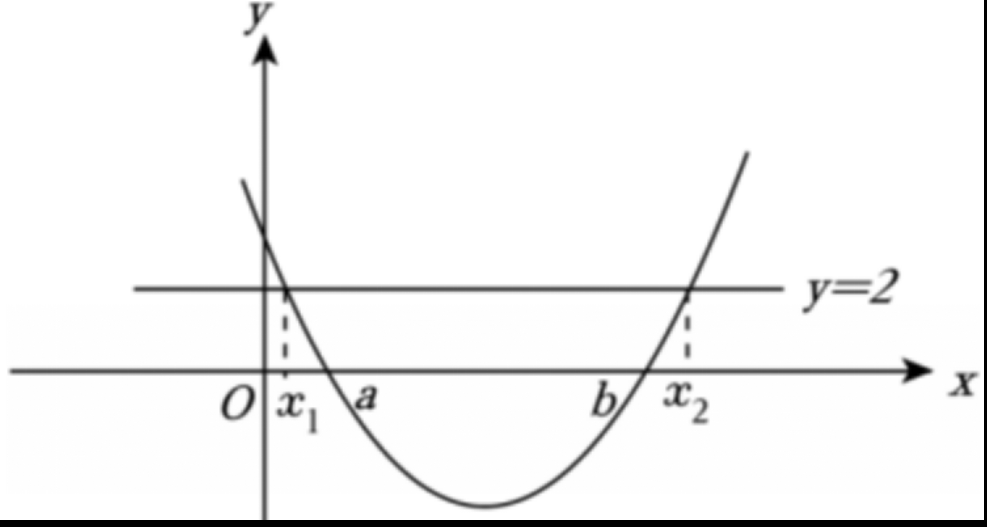
\includegraphics[width=0.42\textwidth]{figures/gao100_q16_parabola.png}
\end{center}
\step{所以数形结合得 $x_1<a<b<x_2$．故选 $B$.}
\solend
\fi

\end{enumerate}

\bigsec{三、解答题}

\begin{enumerate}
\setcounter{enumi}{16}

\item 已知集合 $A=\{x\mid3<x\leqslant6\}$，$B=\{x\mid m\leqslant x\leqslant2m+1\}$.

（1）若 $m=2$，求 $A\cap B$、$A\cup B$；

（2）若 $x\in B$ 是 $x\in A$ 的必要条件，求实数 $m$ 的取值范围.

\ansspace*[9]

\ifanswer
\solbegin
\stepm{（1）}{若 $m=2$，则 $B=\{x\mid2\leqslant x\leqslant5\}$，因为 $A=\{x\mid3<x\leqslant6\}$，}
\step{所以 $A\cap B=\{x\mid3<x\leqslant5\}$，$A\cup B=\{x\mid2\leqslant x\leqslant6\}$.}
\stepm{（2）}{因为 $x\in B$ 是 $x\in A$ 的必要条件，所以 $A\subseteq B$，}
\step{所以 $\begin{cases}m\leqslant3\\ 2m+1\geqslant6\end{cases}$，所以 $\dfrac52\leqslant m\leqslant3$，所以实数 $m$ 的取值范围为 $\left[\dfrac52,3\right]$.}
\solend
\fi

\item 求关于 $x$ 的不等式 $3ax^2-(3a+2)x+2<0\,(a\in R)$ 的解集.

\ansspace*[10]

\ifanswer
\solbegin
\step{当 $a=0$ 时，不等式化为 $-2x+2<0$，解得 $x>1$，}
\step{当 $a\neq0$ 时，方程 $3ax^2-(3a+2)x+2=0$ 的两根分别为 $1$，$\dfrac2{3a}$}
\step{当 $\dfrac2{3a}=1$，即 $a=\dfrac23$ 时，不等式化为 $(x-1)^2<0$，不等式无解，}
\step{当 $\dfrac2{3a}<1$，即 $a>\dfrac23$ 时，不等式解集为 $\left(\dfrac2{3a},1\right)$，}
\step{当 $0<a<\dfrac23$ 时，$\dfrac2{3a}>1$，不等式的解集为 $\left(1,\dfrac2{3a}\right)$，}
\step{当 $a<0$ 时，不等式的解集为 $\left(-\infty,\dfrac2{3a}\right)\cup(1,+\infty)$，}
\step{综上，当 $a=0$ 时，不等式的解集为 $(1,+\infty)$，}
\step{当 $a=\dfrac23$ 时，不等式的解集为 $\varnothing$，}
\step{当 $a>\dfrac23$ 时，不等式解集为 $\left(\dfrac2{3a},1\right)$，}
\step{当 $0<a<\dfrac23$ 时，不等式的解集为 $\left(1,\dfrac2{3a}\right)$，}
\step{当 $a<0$ 时，不等式的解集为 $\left(-\infty,\dfrac2{3a}\right)\cup(1,+\infty)$.}
\solend
\fi

\item 设对于任意实数 $x$，不等式 $\lvert x+1\rvert+\lvert x-1\rvert\geqslant m$ 恒成立.

（1）求 $m$ 的取值范围；

（2）当 $m$ 取最大值时，解关于 $x$ 的不等式 $\lvert x-3\rvert-2x\leqslant2m-2$.

\ansspace*[9]

\ifanswer
\solbegin
\stepm{（1）}{设函数 $f(x)=\lvert x+1\rvert+\lvert x-1\rvert$，则 $f(x)=\begin{cases}-2x,&x\leqslant-1\\ 2,&-1<x<1\\ 2x,&x\geqslant1\end{cases}$，}
\step{当 $x\leqslant-1$ 时，$f(x)$ 有最小值 2；}
\step{当 $-1<x<1$ 时，$f(x)=2$；}
\step{当 $x\geqslant1$ 时，$f(x)$ 有最小值 2；}
\step{因为对于任意实数 $x$，不等式 $\lvert x+1\rvert+\lvert x-1\rvert\geqslant m$ 恒成立，}
\step{所以 $m\leqslant2$，即 $m$ 的取值范围为 $(-\infty,2]$；}
\stepm{（2）}{由（1）得 $m$ 的最大值为 2，所以原不等式为 $\lvert x-3\rvert\leqslant2x+2$，}
\step{即 $-2x-2\leqslant x-3\leqslant2x+2$，解得 $x\geqslant\dfrac13$，}
\step{所以原不等式的解集为 $\left\{x\mid x\geqslant\dfrac13\right\}$.}
\solend
\fi

\item 某轮船公司的一艘轮船每小时花费的燃料费与轮船航行速度的平方成正比，比例系数为 $k$．轮船的最大速度为 18 海里/小时．当船速为 10 海里/小时，它的燃料费是每小时 120 元，其余航行运作费用（不论速度如何）总计是每小时 120 元．假定运行过程中轮船以速度 $v$ 匀速航行.

（1）求 $k$ 的值及每小时的最大总费用 $H$；

（2）求该轮船航行 100 海里的总费用 $W$（燃料费＋其余航行运作费用）的最小值.

\ansspace*[10]

\ifanswer
\solbegin
\stepm{（1）}{由题意，每小时燃料费为 $h(v)=kv^2$，$0<v\leqslant18$，}
\step{已知 $v=10$ 时，燃料费每小时 120 元，则 $k\cdot10^2=120$，得 $k=1.2$，}
\step{每小时总费用 $h(v)=kv^2+120=1.2v^2+120$，}
\step{$h(v)$ 是关于 $v$ 的增函数，$v$ 最大为 18，}
\step{所以 $H=h(18)=1.2\times18^2+120=508.8$ 元.}
\stepm{（2）}{航行时间 $t=\dfrac{100}v$ 小时，}
\step{$W(v)=h(v)\cdot t=(1.2v^2+120)\cdot\dfrac{100}v,0<v\leqslant18=120v+\dfrac{12000}v$，}
\step{利用均值不等式 $120v+\dfrac{12000}v\geqslant2\sqrt{120v\cdot\dfrac{12000}v}=2\times1200=2400$，}
\step{当且仅当 $120v=\dfrac{12000}v$，即 $v=10$ 时取等号，}
\step{$v=10\leqslant18$，在速度范围内，可取到等号，所以总费用最小值为 2400 元.}
\solend
\fi

\item 已知 $A$ 是 $R$ 的非空真子集，如果对任意 $x$、$y\in A$，都有 $x+y\in A$，$xy\in A$，则称 $A$ 是封闭集.

（1）判断集合 $B=\{0\}$，$C=\{-1,0,1\}$ 是否为封闭集，并说明理由；

（2）判断以下两个命题的真假，并说明理由；

命题 $p$：若非空集合 $A_1$、$A_2$ 是封闭集，则 $A_1\cup A_2$ 也是封闭集；

命题 $q$：非空集合 $A_1$、$A_2$ 是封闭集，则 $A_1\cap A_2\neq\varnothing$ 是 $A_1\cap A_2$ 是封闭集的充要条件；

（3）若非空集合 $A$ 是封闭集合，设全集为 $R$，求证：$A$ 的补集不是封闭集.

\ansspace*[13]

\ifanswer
\solbegin
\stepm{（1）}{$B=\{0\}$ 是封闭集，$C=\{-1,0,1\}$ 不是封闭集，理由如下：}
\step{对于集合 $B=\{0\}$，因为 $0+0=0\in B$，$0\times0=0\in B$，}
\step{所以 $B=\{0\}$ 是封闭集；}
\step{对于集合 $C=\{-1,0,1\}$，因为 $-1+(-1)=-2\notin C$，$1+1=2\notin C$，}
\step{所以集合 $C=\{-1,0,1\}$ 不是封闭集.}
\stepm{（2）}{命题 $p$ 是假命题，命题 $q$ 是真命题，理由如下：}
\step{对命题 $p$：令 $A_1=\{x\mid x=2k,k\in Z\}$，$A_2=\{x\mid x=3k,k\in Z\}$，}
\step{令 $x_1=2k_1$，$y_1=2k_2$，$k_1$、$k_2\in Z$，}
\step{则 $x_1+y_1=2(k_1+k_2)\in A_1$，$x_1y_1=2(2k_1k_2)\in A_1$，}
\step{因此集合 $A_1$ 是封闭集，同理集合 $A_2$ 也是封闭集，}
\step{取 $x_2=2$，$y_2=3$，则 $x_2$、$y_2\in(A_1\cup A_2)$，而 $x_2+y_2=5\notin(A_1\cup A_2)$，}
\step{因此集合 $A_1\cup A_2$ 不是封闭集，命题 $p$ 是假命题；}
\step{对于命题 $q$：若 $A_1\cap A_2\neq\varnothing$，不妨令 $a$、$b\in(A_1\cap A_2)$，}
\step{则有 $a$、$b\in A_1$，又集合 $A_1$ 是封闭集，则 $a+b\in A_1$，$ab\in A_1$，}
\step{同理 $a+b\in A_2$，$ab\in A_2$，因此 $a+b\in(A_1\cap A_2)$，$ab\in(A_1\cap A_2)$，}
\step{所以 $A_1\cap A_2$ 是封闭集；}
\step{反之，若 $A_1\cap A_2$ 是封闭集，则 $A_1\cap A_2$ 是非空集合，即 $A_1\cap A_2\neq\varnothing$，}
\step{所以 $A_1\cap A_2$ 是 $A_1\cap A_2$ 是封闭集的充要条件，命题 $q$ 是真命题.}
\stepm{（3）}{非空集合 $A$ 是封闭集合，当 $A=R$ 时，$\overline A=\varnothing$，因此 $\overline A$ 不是封闭集合；}
\step{当 $A\neq R$ 时，假设 $\overline A$ 是封闭集合，}
\step{设 $0\in A$，在 $\overline A$ 中任取一个 $x$，$x\neq0$，则 $-x\in A$，}
\step{否则 $-x\in\overline A$，此时 $x+(-x)=0\in\overline A$，与 $0\in A$ 矛盾，}
\step{因此 $(-x)^2\in A$，$x^2\in\overline A$，而 $(-x)^2=x^2$，与 $A\cap\overline A=\varnothing$ 矛盾，}
\step{则当 $0\in A$ 时，则 $\overline A$ 不是封闭集合，同理当 $0\in\overline A$ 时，$\overline A$ 不是封闭集合，}
\step{所以 $A$ 的补集不是封闭集.}
\solend
\fi

\end{enumerate}

\end{document}
"
%
% 原始材料：微信公众号“魔都数学加油站”文章，连载“27学年高一100”；
% 原文标题“27学年高一100——2026-2027年上海市南洋中学高一上10月月考”；
% 原文链接：https://mp.weixin.qq.com/s/uXLyt6VHraW4hSpDwnZDuQ。
% 正文为 10 张 PNG 页（`原图/高一100_南洋中学_10月月考/01..10.png`），
% 尺寸混排（第 2、4—9 页为 4762×6735，第 1、3、10 页为 2560×3620），按页序读取。
%
% 篇幅与题号：原卷自第 3 题起编号（第 1、2 题不在原文内）。填空题 3—12（10 题）、
% 选择题 13—16（4 题）、解答题 17—21（5 题），共 19 题。
%
% 讲评版：全部 19 题均印【解析】，其中第 13—16 题的答案在解析末句
% “故选 $C$／$B$／$D$／$B$”（题干括号内未印答案）。第 16 题解析带一幅
% 抛物线与 $y=2$ 的示意图，自原图裁切、去粉色水印后转灰度，三版都出。
%
% 副标题：原卷未印副标题。本稿按内容标作“集合与常用逻辑用语、不等式”。
%
% 原卷笔误/存疑（均照录未改，正文对应处另有 % 注）：无。
%
% 与原卷的排版差异：
%   ① 原卷每题下直接印【解析】，本稿按全稿惯例将答案与解析置于答案版；
%   ② 原卷未印副标题，本稿补出；填空横线统一排 \blankline[4.4em]；
%   ③ 原卷数集记号排斜体 $R$、$Z$、$\mathit N$，本稿按全稿惯例改用 $\R$、$\Z$、$\N$；
%   ④ 解答题按惯例加 \ansspace；选择题括号排 \mbox{（\quad）}；
%   ⑤ 第 16 题的示意图原卷排在解析行右侧，本稿改排为解析后的居中图。
%
% 行数核对：逐题数 \step/\stepm 条数，合计 117 条（Q3：2；Q4：5；Q5：7；Q6：3；Q7：3；
% Q8：4；Q9：2；Q10：4；Q11：6；Q12：3；Q13：7；Q14：3；Q15：5；Q16：3；Q17：5；
% Q18：11；Q19：9；Q20：10；Q21：25）。全卷 19 题均印【解析】。
% 原卷解析的换行按语意合并，未逐行强拆。
%
\documentclass[a4paper,11pt]{article}
\usepackage{common}
\begin{document}

\examtitlest[7]{2026--2027 年南洋中学高一上 10 月月考}{集合与常用逻辑用语、不等式}

\bigsec{一、填空题}

\begin{enumerate}
\setcounter{enumi}{2}

\item 不等式 $\dfrac{x-6}{x+1}\geqslant0$ 的解集为\blankline[4.4em].

\ifanswer
\solbegin
\step{不等式 $\dfrac{x-6}{x+1}\geqslant0$ 等价于 $\begin{cases}(x-6)(x+1)\geqslant0\\ x+1\neq0\end{cases}$，即 $x<-1$ 或 $x\geqslant6$，}
\step{故解集为 $(-\infty,-1)\cup[6,+\infty)$.}
\solend
\fi

\item 已知关于 $x$ 的不等式 $ax^2+bx+c>0$ 的解集是 $(1,3)$，则关于 $x$ 的不等式 $ax^2-bx+c\leqslant0$ 的解集为\blankline[4.4em].

\ifanswer
\solbegin
\step{由已知得 $a<0$，且 $1$，$3$ 是方程 $ax^2+bx+c=0$ 的根，}
\step{所以 $\begin{cases}1+3=-\dfrac ba\\[2pt] 1\times3=\dfrac ca\end{cases}$，所以 $\begin{cases}b=-4a\\ c=3a\end{cases}$，}
\step{所以 $ax^2-bx+c\leqslant0$ 可变形为 $ax^2+4ax+3a\leqslant0$，}
\step{因为 $a<0$，所以 $x^2+4x+3\geqslant0$，解得 $x\leqslant-3$ 或 $x\geqslant-1$，}
\step{所以不等式的解集为 $(-\infty,-3]\cup[-1,+\infty)$.}
\solend
\fi

\item 不等式 $\lvert x+2\rvert+\lvert 2x-1\rvert\geqslant3$ 的解集为\blankline[4.4em].

\ifanswer
\solbegin
\step{当 $x\leqslant-2$ 时，$x+2\leqslant0$，$2x-1<0$，}
\step{所以 $\lvert x+2\rvert+\lvert 2x-1\rvert=-x-2-2x+1\geqslant3$，解得 $x\leqslant-\dfrac43$；}
\step{当 $-2<x<\dfrac12$ 时，$x+2>0$，$2x-1<0$，}
\step{所以 $\lvert x+2\rvert+\lvert 2x-1\rvert=x+2-2x+1\geqslant3$，解得 $x\leqslant0$；}
\step{当 $x\geqslant\dfrac12$ 时，$x+2>0$，$2x-1\geqslant0$，}
\step{所以 $\lvert x+2\rvert+\lvert 2x-1\rvert=x+2+2x-1\geqslant3$，解得 $x\geqslant\dfrac23$；}
\step{所以原不等式的解集为 $\left\{x\mid x\leqslant0\right.$ 或 $\left.x\geqslant\dfrac23\right\}$.}
\solend
\fi

\item 若正数 $x$、$y$ 满足 $x+2y=2$，则 $\dfrac1x+\dfrac2y$ 的最小值是\blankline[4.4em].

\ifanswer
\solbegin
\step{因为 $x>0$，$y>0$，且 $x+2y=2$，}
\step{所以 $\dfrac1x+\dfrac2y=\dfrac12\left(\dfrac1x+\dfrac2y\right)(x+2y)=\dfrac12\left(5+\dfrac{2y}x+\dfrac{2x}y\right)\geqslant\dfrac12\left(5+2\sqrt{\dfrac{2y}x\cdot\dfrac{2x}y}\right)=\dfrac92$.}
\step{当且仅当 $\begin{cases}x+2y=2\\ \dfrac{2y}x=\dfrac{2x}y\end{cases}$，即 $x=y=\dfrac23$ 时取等号，故最小值为 $\dfrac92$.}
\solend
\fi

\item 已知 $\alpha:x\leqslant2$ 或 $x>3$，$\beta:x\leqslant m+5$ 或 $x>-m$，若 $\alpha$ 是 $\beta$ 的必要非充分条件，则实数 $m$ 的取值范围是\blankline[4.4em].

\ifanswer
\solbegin
\step{设 $A=\{x\mid x\leqslant2$ 或 $x>3\}$，$B=\{x\mid x\leqslant m+5$ 或 $x>-m\}$，则 $B\subset A$，}
\step{则 $m+5\leqslant2$ 且 $-m\geqslant3$（等号不能同时取得），则 $m<-3$，}
\step{则实数 $m$ 的取值范围是 $(-\infty,-3)$.}
\solend
\fi

\item 已知集合 $A=\{x\mid-1\leqslant x\leqslant3\}$，$B=\{x\mid ax+1>0\}$ 满足 $A\subseteq B$，则实数 $a$ 的取值范围为\blankline[4.4em].

\ifanswer
\solbegin
\step{当 $a=0$ 时，$B=R$，显然符合题意，}
\step{当 $a>0$ 时，$B=\left\{x\mid x>-\dfrac1a\right\}$，则 $-\dfrac1a<-1$，解得 $a<1$，所以 $0<a<1$，}
\step{当 $a<0$ 时，$B=\left\{x\mid x<-\dfrac1a\right\}$，则 $-\dfrac1a>3$，解得 $a>-\dfrac13$，所以 $-\dfrac13<a<0$，}
\step{综上所述，实数 $a$ 的取值范围为 $\left(-\dfrac13,1\right)$.}
\solend
\fi

\item 设集合 $A=\{x\mid3x-1<m\}$，若 $1\in A$ 且 $2\notin A$，则实数 $m$ 的取值范围是\blankline[4.4em].

\ifanswer
\solbegin
\step{因为集合 $A=\{x\mid3x-1<m\}$，若 $1\in A$ 且 $2\notin A$，}
\step{则 $3\times1-1<m$ 且 $3\times2-1\geqslant m$，解得 $2<m\leqslant5$.}
\solend
\fi

\item 若 $M=\left\{x\mid x=m+\dfrac16,m\in Z\right\},N=\left\{x\mid x=\dfrac n2-\dfrac13,n\in Z\right\}$，\newline $P=\left\{x\mid x=\dfrac p2+\dfrac16,p\in Z\right\}$，则 $M$、$N$、$P$ 的关系为\blankline[4.4em].

\ifanswer
\solbegin
\step{$M=\left\{x\mid x=m+\dfrac16=\dfrac{6m+1}6=\dfrac{3\cdot2m+1}6,m\in Z\right\}$，}
\step{$N=\left\{x\mid x=\dfrac n2-\dfrac13=\dfrac{3(n-1)+1}6,n\in Z\right\}=\left\{x\mid x=\dfrac{3k+1}6,k\in Z\right\}$，}
\step{$P=\left\{x\mid x=\dfrac p2+\dfrac16=\dfrac{3p+1}6,p\in Z\right\}$，}
\step{故 $M\subset N=P$.}
\solend
\fi

\item 已知命题 $p:x<-2$ 或 $x>3$，命题 $q:x<3m+1$ 或 $x>m+2$，若 $p$ 是 $q$ 的充分非必要条件，则实数 $m$ 的取值范围是\blankline[4.4em].

\ifanswer
\solbegin
\step{设 $A=\{x\mid x<-2$ 或 $x>3\}$，$B=\{x\mid x<3m+1$ 或 $x>m+2\}$，}
\step{若 $p$ 是 $q$ 的充分非必要条件，则 $A\subset B$，}
\step{当 $3m+1\geqslant m+2$，即 $m\geqslant\dfrac12$ 时，显然有 $A\subset B$，}
\step{当 $3m+1<m+2$，即 $m<\dfrac12$ 时，}
\step{由 $A\subset B$，则 $\begin{cases}m+2\leqslant3\\ 3m+1\geqslant-2\end{cases}$（等号不同时成立），即 $-1\leqslant m<\dfrac12$.}
\step{综上，实数 $m$ 的取值范围是 $[-1,+\infty)$.}
\solend
\fi

\item 对于一个有限集 $A$，一般都可以找到两个非空数集 $A_1$ 和 $A_2$，满足 $A_1\cap A_2=\varnothing$，且 $A_1\cup A_2=A$，记集合 $\{A_1,A_2\}$ 为 $A$ 的一个“划分集”．若 $A$ 中有 $n(n\geqslant2,n\in\N)$ 个元素，则不同的“划分集”共有\blankline[4.4em]个(用含 $n$ 的表达式填空).

\ifanswer
\solbegin
\step{集合中的每个元素都有属于 $A_1$ 或属于 $A_2$ 两种情况，故共有 $2^n$ 种情况，}
\step{排除全都属于 $A_1$ 或 $A_2$ 的两种情况，考虑对称情况，}
\step{故不同的“划分集”共有 $\dfrac12(2^n-2)=2^{n-1}-1$ 个.}
\solend
\fi

\end{enumerate}

\bigsec{二、选择题}

\begin{enumerate}
\setcounter{enumi}{12}

\item 下列命题中正确的\mbox{（\quad）}

\keepwithprev
A. $\varnothing$ 与 $\{0\}$ 表示同一个集合

B. 方程 $\{x\mid(x-2)^2(x-3)=0\}$ 的所有解的集合可表示为 $\{2,2,3\}$

C. 由 3，4，5 组成的集合可表示为 $\{3,4,5\}$ 或 $\{4,5,3\}$

D. 很小的实数可以构成集合.

\ifanswer
\solbegin
\step{对于 $A$，$\{0\}$ 中有一个元素 0，$\varnothing$ 中无任何元素，故 $\varnothing$ 与 $\{0\}$ 不是同一个集合，}
\step{故 $A$ 错误；}
\step{对于 $B$，$\{2,2,3\}$ 不满足集合元素的互异性，故 $B$ 错误；}
\step{对于 $C$，由集合的无序性，得由 3，4，5 组成的集合可表示为 $\{3,4,5\}$ 或 $\{4,5,3\}$，}
\step{故 $C$ 正确；}
\step{对于 $D$，由集合的确定性，很小的实数不能构成集合，故 $D$ 错误.}
\step{故选 $C$.}
\solend
\fi

\item 已知 $a\in R$，则“$\dfrac1a<1$”是“$a>1$”的\mbox{（\quad）}条件.

\keepwithprev
A. 充分非必要\qquad B. 必要非充分

C. 充要\qquad D. 既非充分又非必要

\ifanswer
\solbegin
\step{解 $\dfrac1a<1$，得 $a<0$ 或 $a>1$，}
\step{由 $a<0$ 或 $a>1$ 得不出 $a>1$，由 $a>1$ 得出 $a<0$ 或 $a>1$，}
\step{所以“$\dfrac1a<1$”是“$a>1$”的必要不充分条件．故选 $B$.}
\solend
\fi

\item 若命题“存在 $x_0\in R$ 使得 $ax_0^2+2ax_0+1\leqslant0$”是假命题，则实数 $a$ 的取值范围为\mbox{（\quad）}

\keepwithprev
A. $a<0$ 或 $a\geqslant1$\qquad B. $a\leqslant0$ 或 $a\geqslant1$\qquad C. $0<a<1$\qquad D. $0\leqslant a<1$

\ifanswer
\solbegin
\step{命题“存在 $x_0\in R$ 使得 $ax_0^2+2ax_0+1\leqslant0$”是假命题，}
\step{则 $\forall x\in R$，$ax^2+2ax+1>0$ 恒成立，}
\step{当 $a=0$ 时，满足题意，}
\step{当 $a\neq0$ 时，$\begin{cases}a>0\\ \Delta=4a^2-4a<0\end{cases}$，解得 $0<a<1$，}
\step{综上所述，实数 $a$ 的取值范围为 $\{a\mid0\leqslant a<1\}$．故选 $D$.}
\solend
\fi

\item 已知实数 $a<b$，关于 $x$ 的不等式 $x^2-(a+b)x+ab-2<0$ 的解集为 $(x_1,x_2)$，则实数 $a$、$b$、$x_1$、$x_2$ 从小到大的排列是\mbox{（\quad）}

\keepwithprev
A. $a<x_1<x_2<b$\qquad B. $x_1<a<b<x_2$\qquad C. $a<x_1<b<x_2$\qquad D. $x_1<a<x_2<b$

\ifanswer
\solbegin
\step{因为实数 $a<b$，不等式 $x^2-(a+b)x+ab-2<0$ 可化为 $(x-a)(x-b)<2$，}
\step{又其解集为 $(x_1,x_2)$，所以作出 $y=(x-a)(x-b)$ 与 $y=2$ 的图象如下：}
\begin{center}
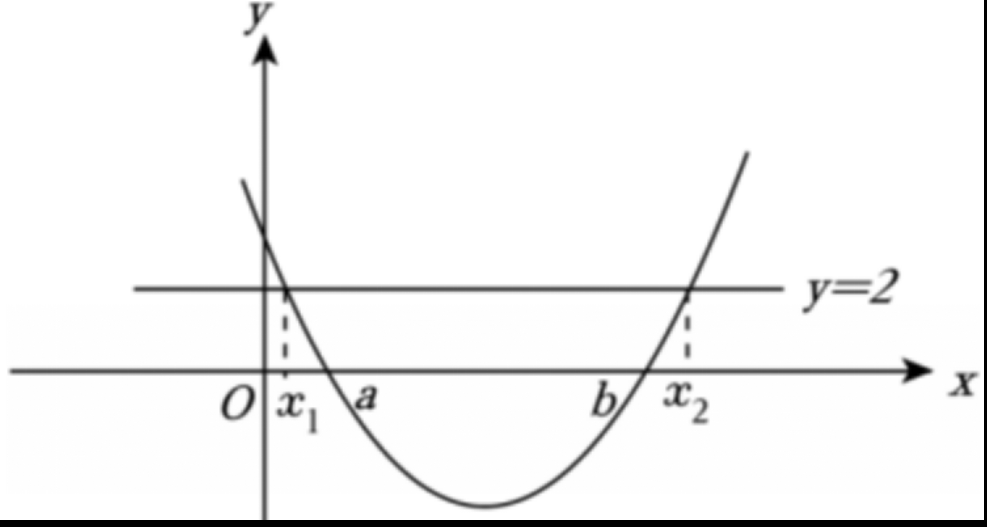
\includegraphics[width=0.42\textwidth]{figures/gao100_q16_parabola.png}
\end{center}
\step{所以数形结合得 $x_1<a<b<x_2$．故选 $B$.}
\solend
\fi

\end{enumerate}

\bigsec{三、解答题}

\begin{enumerate}
\setcounter{enumi}{16}

\item 已知集合 $A=\{x\mid3<x\leqslant6\}$，$B=\{x\mid m\leqslant x\leqslant2m+1\}$.

（1）若 $m=2$，求 $A\cap B$、$A\cup B$；

（2）若 $x\in B$ 是 $x\in A$ 的必要条件，求实数 $m$ 的取值范围.

\ansspace*[9]

\ifanswer
\solbegin
\stepm{（1）}{若 $m=2$，则 $B=\{x\mid2\leqslant x\leqslant5\}$，因为 $A=\{x\mid3<x\leqslant6\}$，}
\step{所以 $A\cap B=\{x\mid3<x\leqslant5\}$，$A\cup B=\{x\mid2\leqslant x\leqslant6\}$.}
\stepm{（2）}{因为 $x\in B$ 是 $x\in A$ 的必要条件，所以 $A\subseteq B$，}
\step{所以 $\begin{cases}m\leqslant3\\ 2m+1\geqslant6\end{cases}$，所以 $\dfrac52\leqslant m\leqslant3$，所以实数 $m$ 的取值范围为 $\left[\dfrac52,3\right]$.}
\solend
\fi

\item 求关于 $x$ 的不等式 $3ax^2-(3a+2)x+2<0\,(a\in R)$ 的解集.

\ansspace*[10]

\ifanswer
\solbegin
\step{当 $a=0$ 时，不等式化为 $-2x+2<0$，解得 $x>1$，}
\step{当 $a\neq0$ 时，方程 $3ax^2-(3a+2)x+2=0$ 的两根分别为 $1$，$\dfrac2{3a}$}
\step{当 $\dfrac2{3a}=1$，即 $a=\dfrac23$ 时，不等式化为 $(x-1)^2<0$，不等式无解，}
\step{当 $\dfrac2{3a}<1$，即 $a>\dfrac23$ 时，不等式解集为 $\left(\dfrac2{3a},1\right)$，}
\step{当 $0<a<\dfrac23$ 时，$\dfrac2{3a}>1$，不等式的解集为 $\left(1,\dfrac2{3a}\right)$，}
\step{当 $a<0$ 时，不等式的解集为 $\left(-\infty,\dfrac2{3a}\right)\cup(1,+\infty)$，}
\step{综上，当 $a=0$ 时，不等式的解集为 $(1,+\infty)$，}
\step{当 $a=\dfrac23$ 时，不等式的解集为 $\varnothing$，}
\step{当 $a>\dfrac23$ 时，不等式解集为 $\left(\dfrac2{3a},1\right)$，}
\step{当 $0<a<\dfrac23$ 时，不等式的解集为 $\left(1,\dfrac2{3a}\right)$，}
\step{当 $a<0$ 时，不等式的解集为 $\left(-\infty,\dfrac2{3a}\right)\cup(1,+\infty)$.}
\solend
\fi

\item 设对于任意实数 $x$，不等式 $\lvert x+1\rvert+\lvert x-1\rvert\geqslant m$ 恒成立.

（1）求 $m$ 的取值范围；

（2）当 $m$ 取最大值时，解关于 $x$ 的不等式 $\lvert x-3\rvert-2x\leqslant2m-2$.

\ansspace*[9]

\ifanswer
\solbegin
\stepm{（1）}{设函数 $f(x)=\lvert x+1\rvert+\lvert x-1\rvert$，则 $f(x)=\begin{cases}-2x,&x\leqslant-1\\ 2,&-1<x<1\\ 2x,&x\geqslant1\end{cases}$，}
\step{当 $x\leqslant-1$ 时，$f(x)$ 有最小值 2；}
\step{当 $-1<x<1$ 时，$f(x)=2$；}
\step{当 $x\geqslant1$ 时，$f(x)$ 有最小值 2；}
\step{因为对于任意实数 $x$，不等式 $\lvert x+1\rvert+\lvert x-1\rvert\geqslant m$ 恒成立，}
\step{所以 $m\leqslant2$，即 $m$ 的取值范围为 $(-\infty,2]$；}
\stepm{（2）}{由（1）得 $m$ 的最大值为 2，所以原不等式为 $\lvert x-3\rvert\leqslant2x+2$，}
\step{即 $-2x-2\leqslant x-3\leqslant2x+2$，解得 $x\geqslant\dfrac13$，}
\step{所以原不等式的解集为 $\left\{x\mid x\geqslant\dfrac13\right\}$.}
\solend
\fi

\item 某轮船公司的一艘轮船每小时花费的燃料费与轮船航行速度的平方成正比，比例系数为 $k$．轮船的最大速度为 18 海里/小时．当船速为 10 海里/小时，它的燃料费是每小时 120 元，其余航行运作费用（不论速度如何）总计是每小时 120 元．假定运行过程中轮船以速度 $v$ 匀速航行.

（1）求 $k$ 的值及每小时的最大总费用 $H$；

（2）求该轮船航行 100 海里的总费用 $W$（燃料费＋其余航行运作费用）的最小值.

\ansspace*[10]

\ifanswer
\solbegin
\stepm{（1）}{由题意，每小时燃料费为 $h(v)=kv^2$，$0<v\leqslant18$，}
\step{已知 $v=10$ 时，燃料费每小时 120 元，则 $k\cdot10^2=120$，得 $k=1.2$，}
\step{每小时总费用 $h(v)=kv^2+120=1.2v^2+120$，}
\step{$h(v)$ 是关于 $v$ 的增函数，$v$ 最大为 18，}
\step{所以 $H=h(18)=1.2\times18^2+120=508.8$ 元.}
\stepm{（2）}{航行时间 $t=\dfrac{100}v$ 小时，}
\step{$W(v)=h(v)\cdot t=(1.2v^2+120)\cdot\dfrac{100}v,0<v\leqslant18=120v+\dfrac{12000}v$，}
\step{利用均值不等式 $120v+\dfrac{12000}v\geqslant2\sqrt{120v\cdot\dfrac{12000}v}=2\times1200=2400$，}
\step{当且仅当 $120v=\dfrac{12000}v$，即 $v=10$ 时取等号，}
\step{$v=10\leqslant18$，在速度范围内，可取到等号，所以总费用最小值为 2400 元.}
\solend
\fi

\item 已知 $A$ 是 $R$ 的非空真子集，如果对任意 $x$、$y\in A$，都有 $x+y\in A$，$xy\in A$，则称 $A$ 是封闭集.

（1）判断集合 $B=\{0\}$，$C=\{-1,0,1\}$ 是否为封闭集，并说明理由；

（2）判断以下两个命题的真假，并说明理由；

命题 $p$：若非空集合 $A_1$、$A_2$ 是封闭集，则 $A_1\cup A_2$ 也是封闭集；

命题 $q$：非空集合 $A_1$、$A_2$ 是封闭集，则 $A_1\cap A_2\neq\varnothing$ 是 $A_1\cap A_2$ 是封闭集的充要条件；

（3）若非空集合 $A$ 是封闭集合，设全集为 $R$，求证：$A$ 的补集不是封闭集.

\ansspace*[13]

\ifanswer
\solbegin
\stepm{（1）}{$B=\{0\}$ 是封闭集，$C=\{-1,0,1\}$ 不是封闭集，理由如下：}
\step{对于集合 $B=\{0\}$，因为 $0+0=0\in B$，$0\times0=0\in B$，}
\step{所以 $B=\{0\}$ 是封闭集；}
\step{对于集合 $C=\{-1,0,1\}$，因为 $-1+(-1)=-2\notin C$，$1+1=2\notin C$，}
\step{所以集合 $C=\{-1,0,1\}$ 不是封闭集.}
\stepm{（2）}{命题 $p$ 是假命题，命题 $q$ 是真命题，理由如下：}
\step{对命题 $p$：令 $A_1=\{x\mid x=2k,k\in Z\}$，$A_2=\{x\mid x=3k,k\in Z\}$，}
\step{令 $x_1=2k_1$，$y_1=2k_2$，$k_1$、$k_2\in Z$，}
\step{则 $x_1+y_1=2(k_1+k_2)\in A_1$，$x_1y_1=2(2k_1k_2)\in A_1$，}
\step{因此集合 $A_1$ 是封闭集，同理集合 $A_2$ 也是封闭集，}
\step{取 $x_2=2$，$y_2=3$，则 $x_2$、$y_2\in(A_1\cup A_2)$，而 $x_2+y_2=5\notin(A_1\cup A_2)$，}
\step{因此集合 $A_1\cup A_2$ 不是封闭集，命题 $p$ 是假命题；}
\step{对于命题 $q$：若 $A_1\cap A_2\neq\varnothing$，不妨令 $a$、$b\in(A_1\cap A_2)$，}
\step{则有 $a$、$b\in A_1$，又集合 $A_1$ 是封闭集，则 $a+b\in A_1$，$ab\in A_1$，}
\step{同理 $a+b\in A_2$，$ab\in A_2$，因此 $a+b\in(A_1\cap A_2)$，$ab\in(A_1\cap A_2)$，}
\step{所以 $A_1\cap A_2$ 是封闭集；}
\step{反之，若 $A_1\cap A_2$ 是封闭集，则 $A_1\cap A_2$ 是非空集合，即 $A_1\cap A_2\neq\varnothing$，}
\step{所以 $A_1\cap A_2$ 是 $A_1\cap A_2$ 是封闭集的充要条件，命题 $q$ 是真命题.}
\stepm{（3）}{非空集合 $A$ 是封闭集合，当 $A=R$ 时，$\overline A=\varnothing$，因此 $\overline A$ 不是封闭集合；}
\step{当 $A\neq R$ 时，假设 $\overline A$ 是封闭集合，}
\step{设 $0\in A$，在 $\overline A$ 中任取一个 $x$，$x\neq0$，则 $-x\in A$，}
\step{否则 $-x\in\overline A$，此时 $x+(-x)=0\in\overline A$，与 $0\in A$ 矛盾，}
\step{因此 $(-x)^2\in A$，$x^2\in\overline A$，而 $(-x)^2=x^2$，与 $A\cap\overline A=\varnothing$ 矛盾，}
\step{则当 $0\in A$ 时，则 $\overline A$ 不是封闭集合，同理当 $0\in\overline A$ 时，$\overline A$ 不是封闭集合，}
\step{所以 $A$ 的补集不是封闭集.}
\solend
\fi

\end{enumerate}

\end{document}
"
%
% 原始材料：微信公众号“魔都数学加油站”文章，连载“27学年高一100”；
% 原文标题“27学年高一100——2026-2027年上海市南洋中学高一上10月月考”；
% 原文链接：https://mp.weixin.qq.com/s/uXLyt6VHraW4hSpDwnZDuQ。
% 正文为 10 张 PNG 页（`原图/高一100_南洋中学_10月月考/01..10.png`），
% 尺寸混排（第 2、4—9 页为 4762×6735，第 1、3、10 页为 2560×3620），按页序读取。
%
% 篇幅与题号：原卷自第 3 题起编号（第 1、2 题不在原文内）。填空题 3—12（10 题）、
% 选择题 13—16（4 题）、解答题 17—21（5 题），共 19 题。
%
% 讲评版：全部 19 题均印【解析】，其中第 13—16 题的答案在解析末句
% “故选 $C$／$B$／$D$／$B$”（题干括号内未印答案）。第 16 题解析带一幅
% 抛物线与 $y=2$ 的示意图，自原图裁切、去粉色水印后转灰度，三版都出。
%
% 副标题：原卷未印副标题。本稿按内容标作“集合与常用逻辑用语、不等式”。
%
% 原卷笔误/存疑（均照录未改，正文对应处另有 % 注）：无。
%
% 与原卷的排版差异：
%   ① 原卷每题下直接印【解析】，本稿按全稿惯例将答案与解析置于答案版；
%   ② 原卷未印副标题，本稿补出；填空横线统一排 \blankline[4.4em]；
%   ③ 原卷数集记号排斜体 $R$、$Z$、$\mathit N$，本稿按全稿惯例改用 $\R$、$\Z$、$\N$；
%   ④ 解答题按惯例加 \ansspace；选择题括号排 \mbox{（\quad）}；
%   ⑤ 第 16 题的示意图原卷排在解析行右侧，本稿改排为解析后的居中图。
%
% 行数核对：逐题数 \step/\stepm 条数，合计 117 条（Q3：2；Q4：5；Q5：7；Q6：3；Q7：3；
% Q8：4；Q9：2；Q10：4；Q11：6；Q12：3；Q13：7；Q14：3；Q15：5；Q16：3；Q17：5；
% Q18：11；Q19：9；Q20：10；Q21：25）。全卷 19 题均印【解析】。
% 原卷解析的换行按语意合并，未逐行强拆。
%
\documentclass[a4paper,11pt]{article}
\usepackage{common}
\begin{document}

\examtitlest[7]{2026--2027 年南洋中学高一上 10 月月考}{集合与常用逻辑用语、不等式}

\bigsec{一、填空题}

\begin{enumerate}
\setcounter{enumi}{2}

\item 不等式 $\dfrac{x-6}{x+1}\geqslant0$ 的解集为\blankline[4.4em].

\ifanswer
\solbegin
\step{不等式 $\dfrac{x-6}{x+1}\geqslant0$ 等价于 $\begin{cases}(x-6)(x+1)\geqslant0\\ x+1\neq0\end{cases}$，即 $x<-1$ 或 $x\geqslant6$，}
\step{故解集为 $(-\infty,-1)\cup[6,+\infty)$.}
\solend
\fi

\item 已知关于 $x$ 的不等式 $ax^2+bx+c>0$ 的解集是 $(1,3)$，则关于 $x$ 的不等式 $ax^2-bx+c\leqslant0$ 的解集为\blankline[4.4em].

\ifanswer
\solbegin
\step{由已知得 $a<0$，且 $1$，$3$ 是方程 $ax^2+bx+c=0$ 的根，}
\step{所以 $\begin{cases}1+3=-\dfrac ba\\[2pt] 1\times3=\dfrac ca\end{cases}$，所以 $\begin{cases}b=-4a\\ c=3a\end{cases}$，}
\step{所以 $ax^2-bx+c\leqslant0$ 可变形为 $ax^2+4ax+3a\leqslant0$，}
\step{因为 $a<0$，所以 $x^2+4x+3\geqslant0$，解得 $x\leqslant-3$ 或 $x\geqslant-1$，}
\step{所以不等式的解集为 $(-\infty,-3]\cup[-1,+\infty)$.}
\solend
\fi

\item 不等式 $\lvert x+2\rvert+\lvert 2x-1\rvert\geqslant3$ 的解集为\blankline[4.4em].

\ifanswer
\solbegin
\step{当 $x\leqslant-2$ 时，$x+2\leqslant0$，$2x-1<0$，}
\step{所以 $\lvert x+2\rvert+\lvert 2x-1\rvert=-x-2-2x+1\geqslant3$，解得 $x\leqslant-\dfrac43$；}
\step{当 $-2<x<\dfrac12$ 时，$x+2>0$，$2x-1<0$，}
\step{所以 $\lvert x+2\rvert+\lvert 2x-1\rvert=x+2-2x+1\geqslant3$，解得 $x\leqslant0$；}
\step{当 $x\geqslant\dfrac12$ 时，$x+2>0$，$2x-1\geqslant0$，}
\step{所以 $\lvert x+2\rvert+\lvert 2x-1\rvert=x+2+2x-1\geqslant3$，解得 $x\geqslant\dfrac23$；}
\step{所以原不等式的解集为 $\left\{x\mid x\leqslant0\right.$ 或 $\left.x\geqslant\dfrac23\right\}$.}
\solend
\fi

\item 若正数 $x$、$y$ 满足 $x+2y=2$，则 $\dfrac1x+\dfrac2y$ 的最小值是\blankline[4.4em].

\ifanswer
\solbegin
\step{因为 $x>0$，$y>0$，且 $x+2y=2$，}
\step{所以 $\dfrac1x+\dfrac2y=\dfrac12\left(\dfrac1x+\dfrac2y\right)(x+2y)=\dfrac12\left(5+\dfrac{2y}x+\dfrac{2x}y\right)\geqslant\dfrac12\left(5+2\sqrt{\dfrac{2y}x\cdot\dfrac{2x}y}\right)=\dfrac92$.}
\step{当且仅当 $\begin{cases}x+2y=2\\ \dfrac{2y}x=\dfrac{2x}y\end{cases}$，即 $x=y=\dfrac23$ 时取等号，故最小值为 $\dfrac92$.}
\solend
\fi

\item 已知 $\alpha:x\leqslant2$ 或 $x>3$，$\beta:x\leqslant m+5$ 或 $x>-m$，若 $\alpha$ 是 $\beta$ 的必要非充分条件，则实数 $m$ 的取值范围是\blankline[4.4em].

\ifanswer
\solbegin
\step{设 $A=\{x\mid x\leqslant2$ 或 $x>3\}$，$B=\{x\mid x\leqslant m+5$ 或 $x>-m\}$，则 $B\subset A$，}
\step{则 $m+5\leqslant2$ 且 $-m\geqslant3$（等号不能同时取得），则 $m<-3$，}
\step{则实数 $m$ 的取值范围是 $(-\infty,-3)$.}
\solend
\fi

\item 已知集合 $A=\{x\mid-1\leqslant x\leqslant3\}$，$B=\{x\mid ax+1>0\}$ 满足 $A\subseteq B$，则实数 $a$ 的取值范围为\blankline[4.4em].

\ifanswer
\solbegin
\step{当 $a=0$ 时，$B=R$，显然符合题意，}
\step{当 $a>0$ 时，$B=\left\{x\mid x>-\dfrac1a\right\}$，则 $-\dfrac1a<-1$，解得 $a<1$，所以 $0<a<1$，}
\step{当 $a<0$ 时，$B=\left\{x\mid x<-\dfrac1a\right\}$，则 $-\dfrac1a>3$，解得 $a>-\dfrac13$，所以 $-\dfrac13<a<0$，}
\step{综上所述，实数 $a$ 的取值范围为 $\left(-\dfrac13,1\right)$.}
\solend
\fi

\item 设集合 $A=\{x\mid3x-1<m\}$，若 $1\in A$ 且 $2\notin A$，则实数 $m$ 的取值范围是\blankline[4.4em].

\ifanswer
\solbegin
\step{因为集合 $A=\{x\mid3x-1<m\}$，若 $1\in A$ 且 $2\notin A$，}
\step{则 $3\times1-1<m$ 且 $3\times2-1\geqslant m$，解得 $2<m\leqslant5$.}
\solend
\fi

\item 若 $M=\left\{x\mid x=m+\dfrac16,m\in Z\right\},N=\left\{x\mid x=\dfrac n2-\dfrac13,n\in Z\right\}$，\newline $P=\left\{x\mid x=\dfrac p2+\dfrac16,p\in Z\right\}$，则 $M$、$N$、$P$ 的关系为\blankline[4.4em].

\ifanswer
\solbegin
\step{$M=\left\{x\mid x=m+\dfrac16=\dfrac{6m+1}6=\dfrac{3\cdot2m+1}6,m\in Z\right\}$，}
\step{$N=\left\{x\mid x=\dfrac n2-\dfrac13=\dfrac{3(n-1)+1}6,n\in Z\right\}=\left\{x\mid x=\dfrac{3k+1}6,k\in Z\right\}$，}
\step{$P=\left\{x\mid x=\dfrac p2+\dfrac16=\dfrac{3p+1}6,p\in Z\right\}$，}
\step{故 $M\subset N=P$.}
\solend
\fi

\item 已知命题 $p:x<-2$ 或 $x>3$，命题 $q:x<3m+1$ 或 $x>m+2$，若 $p$ 是 $q$ 的充分非必要条件，则实数 $m$ 的取值范围是\blankline[4.4em].

\ifanswer
\solbegin
\step{设 $A=\{x\mid x<-2$ 或 $x>3\}$，$B=\{x\mid x<3m+1$ 或 $x>m+2\}$，}
\step{若 $p$ 是 $q$ 的充分非必要条件，则 $A\subset B$，}
\step{当 $3m+1\geqslant m+2$，即 $m\geqslant\dfrac12$ 时，显然有 $A\subset B$，}
\step{当 $3m+1<m+2$，即 $m<\dfrac12$ 时，}
\step{由 $A\subset B$，则 $\begin{cases}m+2\leqslant3\\ 3m+1\geqslant-2\end{cases}$（等号不同时成立），即 $-1\leqslant m<\dfrac12$.}
\step{综上，实数 $m$ 的取值范围是 $[-1,+\infty)$.}
\solend
\fi

\item 对于一个有限集 $A$，一般都可以找到两个非空数集 $A_1$ 和 $A_2$，满足 $A_1\cap A_2=\varnothing$，且 $A_1\cup A_2=A$，记集合 $\{A_1,A_2\}$ 为 $A$ 的一个“划分集”．若 $A$ 中有 $n(n\geqslant2,n\in\N)$ 个元素，则不同的“划分集”共有\blankline[4.4em]个(用含 $n$ 的表达式填空).

\ifanswer
\solbegin
\step{集合中的每个元素都有属于 $A_1$ 或属于 $A_2$ 两种情况，故共有 $2^n$ 种情况，}
\step{排除全都属于 $A_1$ 或 $A_2$ 的两种情况，考虑对称情况，}
\step{故不同的“划分集”共有 $\dfrac12(2^n-2)=2^{n-1}-1$ 个.}
\solend
\fi

\end{enumerate}

\bigsec{二、选择题}

\begin{enumerate}
\setcounter{enumi}{12}

\item 下列命题中正确的\mbox{（\quad）}

\keepwithprev
A. $\varnothing$ 与 $\{0\}$ 表示同一个集合

B. 方程 $\{x\mid(x-2)^2(x-3)=0\}$ 的所有解的集合可表示为 $\{2,2,3\}$

C. 由 3，4，5 组成的集合可表示为 $\{3,4,5\}$ 或 $\{4,5,3\}$

D. 很小的实数可以构成集合.

\ifanswer
\solbegin
\step{对于 $A$，$\{0\}$ 中有一个元素 0，$\varnothing$ 中无任何元素，故 $\varnothing$ 与 $\{0\}$ 不是同一个集合，}
\step{故 $A$ 错误；}
\step{对于 $B$，$\{2,2,3\}$ 不满足集合元素的互异性，故 $B$ 错误；}
\step{对于 $C$，由集合的无序性，得由 3，4，5 组成的集合可表示为 $\{3,4,5\}$ 或 $\{4,5,3\}$，}
\step{故 $C$ 正确；}
\step{对于 $D$，由集合的确定性，很小的实数不能构成集合，故 $D$ 错误.}
\step{故选 $C$.}
\solend
\fi

\item 已知 $a\in R$，则“$\dfrac1a<1$”是“$a>1$”的\mbox{（\quad）}条件.

\keepwithprev
A. 充分非必要\qquad B. 必要非充分

C. 充要\qquad D. 既非充分又非必要

\ifanswer
\solbegin
\step{解 $\dfrac1a<1$，得 $a<0$ 或 $a>1$，}
\step{由 $a<0$ 或 $a>1$ 得不出 $a>1$，由 $a>1$ 得出 $a<0$ 或 $a>1$，}
\step{所以“$\dfrac1a<1$”是“$a>1$”的必要不充分条件．故选 $B$.}
\solend
\fi

\item 若命题“存在 $x_0\in R$ 使得 $ax_0^2+2ax_0+1\leqslant0$”是假命题，则实数 $a$ 的取值范围为\mbox{（\quad）}

\keepwithprev
A. $a<0$ 或 $a\geqslant1$\qquad B. $a\leqslant0$ 或 $a\geqslant1$\qquad C. $0<a<1$\qquad D. $0\leqslant a<1$

\ifanswer
\solbegin
\step{命题“存在 $x_0\in R$ 使得 $ax_0^2+2ax_0+1\leqslant0$”是假命题，}
\step{则 $\forall x\in R$，$ax^2+2ax+1>0$ 恒成立，}
\step{当 $a=0$ 时，满足题意，}
\step{当 $a\neq0$ 时，$\begin{cases}a>0\\ \Delta=4a^2-4a<0\end{cases}$，解得 $0<a<1$，}
\step{综上所述，实数 $a$ 的取值范围为 $\{a\mid0\leqslant a<1\}$．故选 $D$.}
\solend
\fi

\item 已知实数 $a<b$，关于 $x$ 的不等式 $x^2-(a+b)x+ab-2<0$ 的解集为 $(x_1,x_2)$，则实数 $a$、$b$、$x_1$、$x_2$ 从小到大的排列是\mbox{（\quad）}

\keepwithprev
A. $a<x_1<x_2<b$\qquad B. $x_1<a<b<x_2$\qquad C. $a<x_1<b<x_2$\qquad D. $x_1<a<x_2<b$

\ifanswer
\solbegin
\step{因为实数 $a<b$，不等式 $x^2-(a+b)x+ab-2<0$ 可化为 $(x-a)(x-b)<2$，}
\step{又其解集为 $(x_1,x_2)$，所以作出 $y=(x-a)(x-b)$ 与 $y=2$ 的图象如下：}
\begin{center}
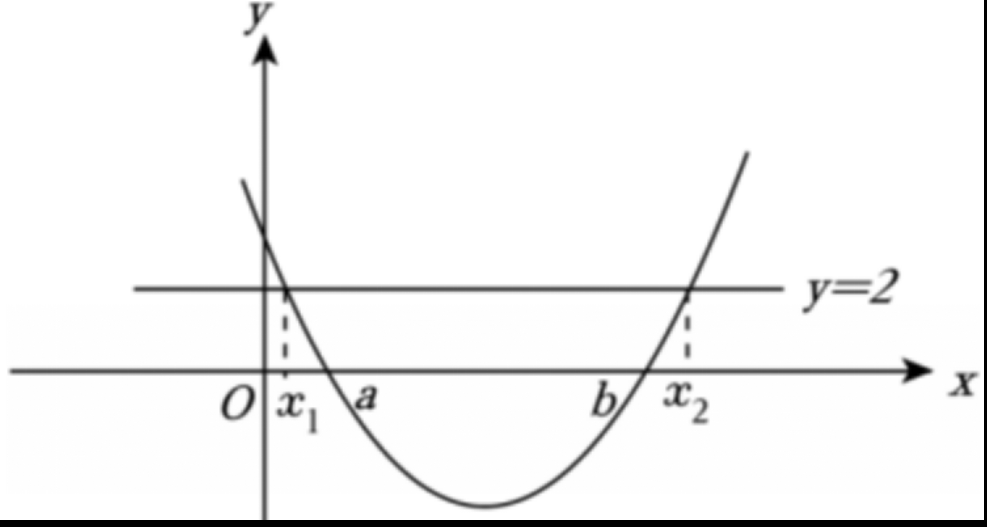
\includegraphics[width=0.42\textwidth]{figures/gao100_q16_parabola.png}
\end{center}
\step{所以数形结合得 $x_1<a<b<x_2$．故选 $B$.}
\solend
\fi

\end{enumerate}

\bigsec{三、解答题}

\begin{enumerate}
\setcounter{enumi}{16}

\item 已知集合 $A=\{x\mid3<x\leqslant6\}$，$B=\{x\mid m\leqslant x\leqslant2m+1\}$.

（1）若 $m=2$，求 $A\cap B$、$A\cup B$；

（2）若 $x\in B$ 是 $x\in A$ 的必要条件，求实数 $m$ 的取值范围.

\ansspace*[9]

\ifanswer
\solbegin
\stepm{（1）}{若 $m=2$，则 $B=\{x\mid2\leqslant x\leqslant5\}$，因为 $A=\{x\mid3<x\leqslant6\}$，}
\step{所以 $A\cap B=\{x\mid3<x\leqslant5\}$，$A\cup B=\{x\mid2\leqslant x\leqslant6\}$.}
\stepm{（2）}{因为 $x\in B$ 是 $x\in A$ 的必要条件，所以 $A\subseteq B$，}
\step{所以 $\begin{cases}m\leqslant3\\ 2m+1\geqslant6\end{cases}$，所以 $\dfrac52\leqslant m\leqslant3$，所以实数 $m$ 的取值范围为 $\left[\dfrac52,3\right]$.}
\solend
\fi

\item 求关于 $x$ 的不等式 $3ax^2-(3a+2)x+2<0\,(a\in R)$ 的解集.

\ansspace*[10]

\ifanswer
\solbegin
\step{当 $a=0$ 时，不等式化为 $-2x+2<0$，解得 $x>1$，}
\step{当 $a\neq0$ 时，方程 $3ax^2-(3a+2)x+2=0$ 的两根分别为 $1$，$\dfrac2{3a}$}
\step{当 $\dfrac2{3a}=1$，即 $a=\dfrac23$ 时，不等式化为 $(x-1)^2<0$，不等式无解，}
\step{当 $\dfrac2{3a}<1$，即 $a>\dfrac23$ 时，不等式解集为 $\left(\dfrac2{3a},1\right)$，}
\step{当 $0<a<\dfrac23$ 时，$\dfrac2{3a}>1$，不等式的解集为 $\left(1,\dfrac2{3a}\right)$，}
\step{当 $a<0$ 时，不等式的解集为 $\left(-\infty,\dfrac2{3a}\right)\cup(1,+\infty)$，}
\step{综上，当 $a=0$ 时，不等式的解集为 $(1,+\infty)$，}
\step{当 $a=\dfrac23$ 时，不等式的解集为 $\varnothing$，}
\step{当 $a>\dfrac23$ 时，不等式解集为 $\left(\dfrac2{3a},1\right)$，}
\step{当 $0<a<\dfrac23$ 时，不等式的解集为 $\left(1,\dfrac2{3a}\right)$，}
\step{当 $a<0$ 时，不等式的解集为 $\left(-\infty,\dfrac2{3a}\right)\cup(1,+\infty)$.}
\solend
\fi

\item 设对于任意实数 $x$，不等式 $\lvert x+1\rvert+\lvert x-1\rvert\geqslant m$ 恒成立.

（1）求 $m$ 的取值范围；

（2）当 $m$ 取最大值时，解关于 $x$ 的不等式 $\lvert x-3\rvert-2x\leqslant2m-2$.

\ansspace*[9]

\ifanswer
\solbegin
\stepm{（1）}{设函数 $f(x)=\lvert x+1\rvert+\lvert x-1\rvert$，则 $f(x)=\begin{cases}-2x,&x\leqslant-1\\ 2,&-1<x<1\\ 2x,&x\geqslant1\end{cases}$，}
\step{当 $x\leqslant-1$ 时，$f(x)$ 有最小值 2；}
\step{当 $-1<x<1$ 时，$f(x)=2$；}
\step{当 $x\geqslant1$ 时，$f(x)$ 有最小值 2；}
\step{因为对于任意实数 $x$，不等式 $\lvert x+1\rvert+\lvert x-1\rvert\geqslant m$ 恒成立，}
\step{所以 $m\leqslant2$，即 $m$ 的取值范围为 $(-\infty,2]$；}
\stepm{（2）}{由（1）得 $m$ 的最大值为 2，所以原不等式为 $\lvert x-3\rvert\leqslant2x+2$，}
\step{即 $-2x-2\leqslant x-3\leqslant2x+2$，解得 $x\geqslant\dfrac13$，}
\step{所以原不等式的解集为 $\left\{x\mid x\geqslant\dfrac13\right\}$.}
\solend
\fi

\item 某轮船公司的一艘轮船每小时花费的燃料费与轮船航行速度的平方成正比，比例系数为 $k$．轮船的最大速度为 18 海里/小时．当船速为 10 海里/小时，它的燃料费是每小时 120 元，其余航行运作费用（不论速度如何）总计是每小时 120 元．假定运行过程中轮船以速度 $v$ 匀速航行.

（1）求 $k$ 的值及每小时的最大总费用 $H$；

（2）求该轮船航行 100 海里的总费用 $W$（燃料费＋其余航行运作费用）的最小值.

\ansspace*[10]

\ifanswer
\solbegin
\stepm{（1）}{由题意，每小时燃料费为 $h(v)=kv^2$，$0<v\leqslant18$，}
\step{已知 $v=10$ 时，燃料费每小时 120 元，则 $k\cdot10^2=120$，得 $k=1.2$，}
\step{每小时总费用 $h(v)=kv^2+120=1.2v^2+120$，}
\step{$h(v)$ 是关于 $v$ 的增函数，$v$ 最大为 18，}
\step{所以 $H=h(18)=1.2\times18^2+120=508.8$ 元.}
\stepm{（2）}{航行时间 $t=\dfrac{100}v$ 小时，}
\step{$W(v)=h(v)\cdot t=(1.2v^2+120)\cdot\dfrac{100}v,0<v\leqslant18=120v+\dfrac{12000}v$，}
\step{利用均值不等式 $120v+\dfrac{12000}v\geqslant2\sqrt{120v\cdot\dfrac{12000}v}=2\times1200=2400$，}
\step{当且仅当 $120v=\dfrac{12000}v$，即 $v=10$ 时取等号，}
\step{$v=10\leqslant18$，在速度范围内，可取到等号，所以总费用最小值为 2400 元.}
\solend
\fi

\item 已知 $A$ 是 $R$ 的非空真子集，如果对任意 $x$、$y\in A$，都有 $x+y\in A$，$xy\in A$，则称 $A$ 是封闭集.

（1）判断集合 $B=\{0\}$，$C=\{-1,0,1\}$ 是否为封闭集，并说明理由；

（2）判断以下两个命题的真假，并说明理由；

命题 $p$：若非空集合 $A_1$、$A_2$ 是封闭集，则 $A_1\cup A_2$ 也是封闭集；

命题 $q$：非空集合 $A_1$、$A_2$ 是封闭集，则 $A_1\cap A_2\neq\varnothing$ 是 $A_1\cap A_2$ 是封闭集的充要条件；

（3）若非空集合 $A$ 是封闭集合，设全集为 $R$，求证：$A$ 的补集不是封闭集.

\ansspace*[13]

\ifanswer
\solbegin
\stepm{（1）}{$B=\{0\}$ 是封闭集，$C=\{-1,0,1\}$ 不是封闭集，理由如下：}
\step{对于集合 $B=\{0\}$，因为 $0+0=0\in B$，$0\times0=0\in B$，}
\step{所以 $B=\{0\}$ 是封闭集；}
\step{对于集合 $C=\{-1,0,1\}$，因为 $-1+(-1)=-2\notin C$，$1+1=2\notin C$，}
\step{所以集合 $C=\{-1,0,1\}$ 不是封闭集.}
\stepm{（2）}{命题 $p$ 是假命题，命题 $q$ 是真命题，理由如下：}
\step{对命题 $p$：令 $A_1=\{x\mid x=2k,k\in Z\}$，$A_2=\{x\mid x=3k,k\in Z\}$，}
\step{令 $x_1=2k_1$，$y_1=2k_2$，$k_1$、$k_2\in Z$，}
\step{则 $x_1+y_1=2(k_1+k_2)\in A_1$，$x_1y_1=2(2k_1k_2)\in A_1$，}
\step{因此集合 $A_1$ 是封闭集，同理集合 $A_2$ 也是封闭集，}
\step{取 $x_2=2$，$y_2=3$，则 $x_2$、$y_2\in(A_1\cup A_2)$，而 $x_2+y_2=5\notin(A_1\cup A_2)$，}
\step{因此集合 $A_1\cup A_2$ 不是封闭集，命题 $p$ 是假命题；}
\step{对于命题 $q$：若 $A_1\cap A_2\neq\varnothing$，不妨令 $a$、$b\in(A_1\cap A_2)$，}
\step{则有 $a$、$b\in A_1$，又集合 $A_1$ 是封闭集，则 $a+b\in A_1$，$ab\in A_1$，}
\step{同理 $a+b\in A_2$，$ab\in A_2$，因此 $a+b\in(A_1\cap A_2)$，$ab\in(A_1\cap A_2)$，}
\step{所以 $A_1\cap A_2$ 是封闭集；}
\step{反之，若 $A_1\cap A_2$ 是封闭集，则 $A_1\cap A_2$ 是非空集合，即 $A_1\cap A_2\neq\varnothing$，}
\step{所以 $A_1\cap A_2$ 是 $A_1\cap A_2$ 是封闭集的充要条件，命题 $q$ 是真命题.}
\stepm{（3）}{非空集合 $A$ 是封闭集合，当 $A=R$ 时，$\overline A=\varnothing$，因此 $\overline A$ 不是封闭集合；}
\step{当 $A\neq R$ 时，假设 $\overline A$ 是封闭集合，}
\step{设 $0\in A$，在 $\overline A$ 中任取一个 $x$，$x\neq0$，则 $-x\in A$，}
\step{否则 $-x\in\overline A$，此时 $x+(-x)=0\in\overline A$，与 $0\in A$ 矛盾，}
\step{因此 $(-x)^2\in A$，$x^2\in\overline A$，而 $(-x)^2=x^2$，与 $A\cap\overline A=\varnothing$ 矛盾，}
\step{则当 $0\in A$ 时，则 $\overline A$ 不是封闭集合，同理当 $0\in\overline A$ 时，$\overline A$ 不是封闭集合，}
\step{所以 $A$ 的补集不是封闭集.}
\solend
\fi

\end{enumerate}

\end{document}
"
%
% 原始材料：微信公众号“魔都数学加油站”文章，连载“27学年高一100”；
% 原文标题“27学年高一100——2026-2027年上海市南洋中学高一上10月月考”；
% 原文链接：https://mp.weixin.qq.com/s/uXLyt6VHraW4hSpDwnZDuQ。
% 正文为 10 张 PNG 页（`原图/高一100_南洋中学_10月月考/01..10.png`），
% 尺寸混排（第 2、4—9 页为 4762×6735，第 1、3、10 页为 2560×3620），按页序读取。
%
% 篇幅与题号：原卷自第 3 题起编号（第 1、2 题不在原文内）。填空题 3—12（10 题）、
% 选择题 13—16（4 题）、解答题 17—21（5 题），共 19 题。
%
% 讲评版：全部 19 题均印【解析】，其中第 13—16 题的答案在解析末句
% “故选 $C$／$B$／$D$／$B$”（题干括号内未印答案）。第 16 题解析带一幅
% 抛物线与 $y=2$ 的示意图，自原图裁切、去粉色水印后转灰度，三版都出。
%
% 副标题：原卷未印副标题。本稿按内容标作“集合与常用逻辑用语、不等式”。
%
% 原卷笔误/存疑（均照录未改，正文对应处另有 % 注）：无。
%
% 与原卷的排版差异：
%   ① 原卷每题下直接印【解析】，本稿按全稿惯例将答案与解析置于答案版；
%   ② 原卷未印副标题，本稿补出；填空横线统一排 \blankline[4.4em]；
%   ③ 原卷数集记号排斜体 $R$、$Z$、$\mathit N$，本稿按全稿惯例改用 $\R$、$\Z$、$\N$；
%   ④ 解答题按惯例加 \ansspace；选择题括号排 \mbox{（\quad）}；
%   ⑤ 第 16 题的示意图原卷排在解析行右侧，本稿改排为解析后的居中图。
%
% 行数核对：逐题数 \step/\stepm 条数，合计 117 条（Q3：2；Q4：5；Q5：7；Q6：3；Q7：3；
% Q8：4；Q9：2；Q10：4；Q11：6；Q12：3；Q13：7；Q14：3；Q15：5；Q16：3；Q17：5；
% Q18：11；Q19：9；Q20：10；Q21：25）。全卷 19 题均印【解析】。
% 原卷解析的换行按语意合并，未逐行强拆。
%
\documentclass[a4paper,11pt]{article}
\usepackage{common}
\begin{document}

\examtitlest[7]{2026--2027 年南洋中学高一上 10 月月考}{集合与常用逻辑用语、不等式}

\bigsec{一、填空题}

\begin{enumerate}
\setcounter{enumi}{2}

\item 不等式 $\dfrac{x-6}{x+1}\geqslant0$ 的解集为\blankline[4.4em].

\ifanswer
\solbegin
\step{不等式 $\dfrac{x-6}{x+1}\geqslant0$ 等价于 $\begin{cases}(x-6)(x+1)\geqslant0\\ x+1\neq0\end{cases}$，即 $x<-1$ 或 $x\geqslant6$，}
\step{故解集为 $(-\infty,-1)\cup[6,+\infty)$.}
\solend
\fi

\item 已知关于 $x$ 的不等式 $ax^2+bx+c>0$ 的解集是 $(1,3)$，则关于 $x$ 的不等式 $ax^2-bx+c\leqslant0$ 的解集为\blankline[4.4em].

\ifanswer
\solbegin
\step{由已知得 $a<0$，且 $1$，$3$ 是方程 $ax^2+bx+c=0$ 的根，}
\step{所以 $\begin{cases}1+3=-\dfrac ba\\[2pt] 1\times3=\dfrac ca\end{cases}$，所以 $\begin{cases}b=-4a\\ c=3a\end{cases}$，}
\step{所以 $ax^2-bx+c\leqslant0$ 可变形为 $ax^2+4ax+3a\leqslant0$，}
\step{因为 $a<0$，所以 $x^2+4x+3\geqslant0$，解得 $x\leqslant-3$ 或 $x\geqslant-1$，}
\step{所以不等式的解集为 $(-\infty,-3]\cup[-1,+\infty)$.}
\solend
\fi

\item 不等式 $\lvert x+2\rvert+\lvert 2x-1\rvert\geqslant3$ 的解集为\blankline[4.4em].

\ifanswer
\solbegin
\step{当 $x\leqslant-2$ 时，$x+2\leqslant0$，$2x-1<0$，}
\step{所以 $\lvert x+2\rvert+\lvert 2x-1\rvert=-x-2-2x+1\geqslant3$，解得 $x\leqslant-\dfrac43$；}
\step{当 $-2<x<\dfrac12$ 时，$x+2>0$，$2x-1<0$，}
\step{所以 $\lvert x+2\rvert+\lvert 2x-1\rvert=x+2-2x+1\geqslant3$，解得 $x\leqslant0$；}
\step{当 $x\geqslant\dfrac12$ 时，$x+2>0$，$2x-1\geqslant0$，}
\step{所以 $\lvert x+2\rvert+\lvert 2x-1\rvert=x+2+2x-1\geqslant3$，解得 $x\geqslant\dfrac23$；}
\step{所以原不等式的解集为 $\left\{x\mid x\leqslant0\right.$ 或 $\left.x\geqslant\dfrac23\right\}$.}
\solend
\fi

\item 若正数 $x$、$y$ 满足 $x+2y=2$，则 $\dfrac1x+\dfrac2y$ 的最小值是\blankline[4.4em].

\ifanswer
\solbegin
\step{因为 $x>0$，$y>0$，且 $x+2y=2$，}
\step{所以 $\dfrac1x+\dfrac2y=\dfrac12\left(\dfrac1x+\dfrac2y\right)(x+2y)=\dfrac12\left(5+\dfrac{2y}x+\dfrac{2x}y\right)\geqslant\dfrac12\left(5+2\sqrt{\dfrac{2y}x\cdot\dfrac{2x}y}\right)=\dfrac92$.}
\step{当且仅当 $\begin{cases}x+2y=2\\ \dfrac{2y}x=\dfrac{2x}y\end{cases}$，即 $x=y=\dfrac23$ 时取等号，故最小值为 $\dfrac92$.}
\solend
\fi

\item 已知 $\alpha:x\leqslant2$ 或 $x>3$，$\beta:x\leqslant m+5$ 或 $x>-m$，若 $\alpha$ 是 $\beta$ 的必要非充分条件，则实数 $m$ 的取值范围是\blankline[4.4em].

\ifanswer
\solbegin
\step{设 $A=\{x\mid x\leqslant2$ 或 $x>3\}$，$B=\{x\mid x\leqslant m+5$ 或 $x>-m\}$，则 $B\subset A$，}
\step{则 $m+5\leqslant2$ 且 $-m\geqslant3$（等号不能同时取得），则 $m<-3$，}
\step{则实数 $m$ 的取值范围是 $(-\infty,-3)$.}
\solend
\fi

\item 已知集合 $A=\{x\mid-1\leqslant x\leqslant3\}$，$B=\{x\mid ax+1>0\}$ 满足 $A\subseteq B$，则实数 $a$ 的取值范围为\blankline[4.4em].

\ifanswer
\solbegin
\step{当 $a=0$ 时，$B=R$，显然符合题意，}
\step{当 $a>0$ 时，$B=\left\{x\mid x>-\dfrac1a\right\}$，则 $-\dfrac1a<-1$，解得 $a<1$，所以 $0<a<1$，}
\step{当 $a<0$ 时，$B=\left\{x\mid x<-\dfrac1a\right\}$，则 $-\dfrac1a>3$，解得 $a>-\dfrac13$，所以 $-\dfrac13<a<0$，}
\step{综上所述，实数 $a$ 的取值范围为 $\left(-\dfrac13,1\right)$.}
\solend
\fi

\item 设集合 $A=\{x\mid3x-1<m\}$，若 $1\in A$ 且 $2\notin A$，则实数 $m$ 的取值范围是\blankline[4.4em].

\ifanswer
\solbegin
\step{因为集合 $A=\{x\mid3x-1<m\}$，若 $1\in A$ 且 $2\notin A$，}
\step{则 $3\times1-1<m$ 且 $3\times2-1\geqslant m$，解得 $2<m\leqslant5$.}
\solend
\fi

\item 若 $M=\left\{x\mid x=m+\dfrac16,m\in Z\right\},N=\left\{x\mid x=\dfrac n2-\dfrac13,n\in Z\right\}$，\newline $P=\left\{x\mid x=\dfrac p2+\dfrac16,p\in Z\right\}$，则 $M$、$N$、$P$ 的关系为\blankline[4.4em].

\ifanswer
\solbegin
\step{$M=\left\{x\mid x=m+\dfrac16=\dfrac{6m+1}6=\dfrac{3\cdot2m+1}6,m\in Z\right\}$，}
\step{$N=\left\{x\mid x=\dfrac n2-\dfrac13=\dfrac{3(n-1)+1}6,n\in Z\right\}=\left\{x\mid x=\dfrac{3k+1}6,k\in Z\right\}$，}
\step{$P=\left\{x\mid x=\dfrac p2+\dfrac16=\dfrac{3p+1}6,p\in Z\right\}$，}
\step{故 $M\subset N=P$.}
\solend
\fi

\item 已知命题 $p:x<-2$ 或 $x>3$，命题 $q:x<3m+1$ 或 $x>m+2$，若 $p$ 是 $q$ 的充分非必要条件，则实数 $m$ 的取值范围是\blankline[4.4em].

\ifanswer
\solbegin
\step{设 $A=\{x\mid x<-2$ 或 $x>3\}$，$B=\{x\mid x<3m+1$ 或 $x>m+2\}$，}
\step{若 $p$ 是 $q$ 的充分非必要条件，则 $A\subset B$，}
\step{当 $3m+1\geqslant m+2$，即 $m\geqslant\dfrac12$ 时，显然有 $A\subset B$，}
\step{当 $3m+1<m+2$，即 $m<\dfrac12$ 时，}
\step{由 $A\subset B$，则 $\begin{cases}m+2\leqslant3\\ 3m+1\geqslant-2\end{cases}$（等号不同时成立），即 $-1\leqslant m<\dfrac12$.}
\step{综上，实数 $m$ 的取值范围是 $[-1,+\infty)$.}
\solend
\fi

\item 对于一个有限集 $A$，一般都可以找到两个非空数集 $A_1$ 和 $A_2$，满足 $A_1\cap A_2=\varnothing$，且 $A_1\cup A_2=A$，记集合 $\{A_1,A_2\}$ 为 $A$ 的一个“划分集”．若 $A$ 中有 $n(n\geqslant2,n\in\N)$ 个元素，则不同的“划分集”共有\blankline[4.4em]个(用含 $n$ 的表达式填空).

\ifanswer
\solbegin
\step{集合中的每个元素都有属于 $A_1$ 或属于 $A_2$ 两种情况，故共有 $2^n$ 种情况，}
\step{排除全都属于 $A_1$ 或 $A_2$ 的两种情况，考虑对称情况，}
\step{故不同的“划分集”共有 $\dfrac12(2^n-2)=2^{n-1}-1$ 个.}
\solend
\fi

\end{enumerate}

\bigsec{二、选择题}

\begin{enumerate}
\setcounter{enumi}{12}

\item 下列命题中正确的\mbox{（\quad）}

\keepwithprev
A. $\varnothing$ 与 $\{0\}$ 表示同一个集合

B. 方程 $\{x\mid(x-2)^2(x-3)=0\}$ 的所有解的集合可表示为 $\{2,2,3\}$

C. 由 3，4，5 组成的集合可表示为 $\{3,4,5\}$ 或 $\{4,5,3\}$

D. 很小的实数可以构成集合.

\ifanswer
\solbegin
\step{对于 $A$，$\{0\}$ 中有一个元素 0，$\varnothing$ 中无任何元素，故 $\varnothing$ 与 $\{0\}$ 不是同一个集合，}
\step{故 $A$ 错误；}
\step{对于 $B$，$\{2,2,3\}$ 不满足集合元素的互异性，故 $B$ 错误；}
\step{对于 $C$，由集合的无序性，得由 3，4，5 组成的集合可表示为 $\{3,4,5\}$ 或 $\{4,5,3\}$，}
\step{故 $C$ 正确；}
\step{对于 $D$，由集合的确定性，很小的实数不能构成集合，故 $D$ 错误.}
\step{故选 $C$.}
\solend
\fi

\item 已知 $a\in R$，则“$\dfrac1a<1$”是“$a>1$”的\mbox{（\quad）}条件.

\keepwithprev
A. 充分非必要\qquad B. 必要非充分

C. 充要\qquad D. 既非充分又非必要

\ifanswer
\solbegin
\step{解 $\dfrac1a<1$，得 $a<0$ 或 $a>1$，}
\step{由 $a<0$ 或 $a>1$ 得不出 $a>1$，由 $a>1$ 得出 $a<0$ 或 $a>1$，}
\step{所以“$\dfrac1a<1$”是“$a>1$”的必要不充分条件．故选 $B$.}
\solend
\fi

\item 若命题“存在 $x_0\in R$ 使得 $ax_0^2+2ax_0+1\leqslant0$”是假命题，则实数 $a$ 的取值范围为\mbox{（\quad）}

\keepwithprev
A. $a<0$ 或 $a\geqslant1$\qquad B. $a\leqslant0$ 或 $a\geqslant1$\qquad C. $0<a<1$\qquad D. $0\leqslant a<1$

\ifanswer
\solbegin
\step{命题“存在 $x_0\in R$ 使得 $ax_0^2+2ax_0+1\leqslant0$”是假命题，}
\step{则 $\forall x\in R$，$ax^2+2ax+1>0$ 恒成立，}
\step{当 $a=0$ 时，满足题意，}
\step{当 $a\neq0$ 时，$\begin{cases}a>0\\ \Delta=4a^2-4a<0\end{cases}$，解得 $0<a<1$，}
\step{综上所述，实数 $a$ 的取值范围为 $\{a\mid0\leqslant a<1\}$．故选 $D$.}
\solend
\fi

\item 已知实数 $a<b$，关于 $x$ 的不等式 $x^2-(a+b)x+ab-2<0$ 的解集为 $(x_1,x_2)$，则实数 $a$、$b$、$x_1$、$x_2$ 从小到大的排列是\mbox{（\quad）}

\keepwithprev
A. $a<x_1<x_2<b$\qquad B. $x_1<a<b<x_2$\qquad C. $a<x_1<b<x_2$\qquad D. $x_1<a<x_2<b$

\ifanswer
\solbegin
\step{因为实数 $a<b$，不等式 $x^2-(a+b)x+ab-2<0$ 可化为 $(x-a)(x-b)<2$，}
\step{又其解集为 $(x_1,x_2)$，所以作出 $y=(x-a)(x-b)$ 与 $y=2$ 的图象如下：}
\begin{center}
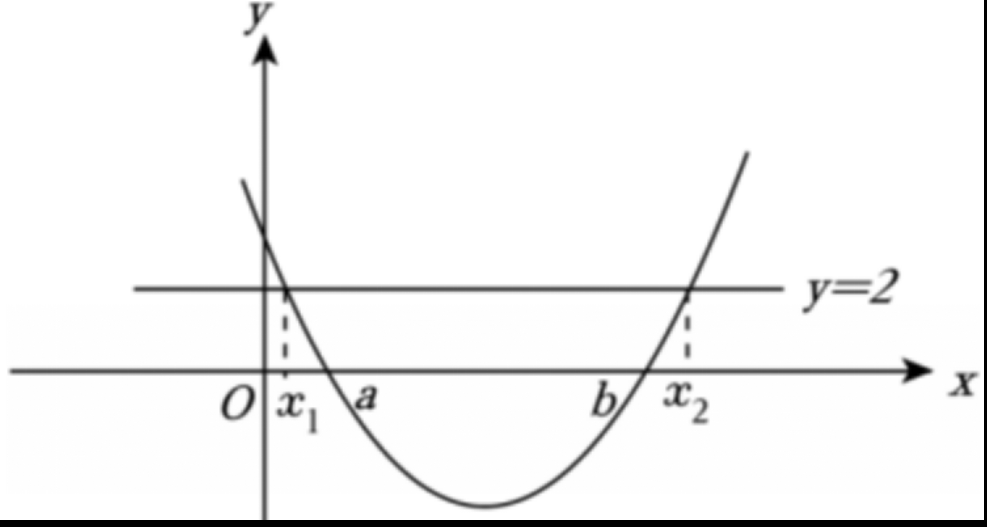
\includegraphics[width=0.42\textwidth]{figures/gao100_q16_parabola.png}
\end{center}
\step{所以数形结合得 $x_1<a<b<x_2$．故选 $B$.}
\solend
\fi

\end{enumerate}

\bigsec{三、解答题}

\begin{enumerate}
\setcounter{enumi}{16}

\item 已知集合 $A=\{x\mid3<x\leqslant6\}$，$B=\{x\mid m\leqslant x\leqslant2m+1\}$.

（1）若 $m=2$，求 $A\cap B$、$A\cup B$；

（2）若 $x\in B$ 是 $x\in A$ 的必要条件，求实数 $m$ 的取值范围.

\ansspace*[9]

\ifanswer
\solbegin
\stepm{（1）}{若 $m=2$，则 $B=\{x\mid2\leqslant x\leqslant5\}$，因为 $A=\{x\mid3<x\leqslant6\}$，}
\step{所以 $A\cap B=\{x\mid3<x\leqslant5\}$，$A\cup B=\{x\mid2\leqslant x\leqslant6\}$.}
\stepm{（2）}{因为 $x\in B$ 是 $x\in A$ 的必要条件，所以 $A\subseteq B$，}
\step{所以 $\begin{cases}m\leqslant3\\ 2m+1\geqslant6\end{cases}$，所以 $\dfrac52\leqslant m\leqslant3$，所以实数 $m$ 的取值范围为 $\left[\dfrac52,3\right]$.}
\solend
\fi

\item 求关于 $x$ 的不等式 $3ax^2-(3a+2)x+2<0\,(a\in R)$ 的解集.

\ansspace*[10]

\ifanswer
\solbegin
\step{当 $a=0$ 时，不等式化为 $-2x+2<0$，解得 $x>1$，}
\step{当 $a\neq0$ 时，方程 $3ax^2-(3a+2)x+2=0$ 的两根分别为 $1$，$\dfrac2{3a}$}
\step{当 $\dfrac2{3a}=1$，即 $a=\dfrac23$ 时，不等式化为 $(x-1)^2<0$，不等式无解，}
\step{当 $\dfrac2{3a}<1$，即 $a>\dfrac23$ 时，不等式解集为 $\left(\dfrac2{3a},1\right)$，}
\step{当 $0<a<\dfrac23$ 时，$\dfrac2{3a}>1$，不等式的解集为 $\left(1,\dfrac2{3a}\right)$，}
\step{当 $a<0$ 时，不等式的解集为 $\left(-\infty,\dfrac2{3a}\right)\cup(1,+\infty)$，}
\step{综上，当 $a=0$ 时，不等式的解集为 $(1,+\infty)$，}
\step{当 $a=\dfrac23$ 时，不等式的解集为 $\varnothing$，}
\step{当 $a>\dfrac23$ 时，不等式解集为 $\left(\dfrac2{3a},1\right)$，}
\step{当 $0<a<\dfrac23$ 时，不等式的解集为 $\left(1,\dfrac2{3a}\right)$，}
\step{当 $a<0$ 时，不等式的解集为 $\left(-\infty,\dfrac2{3a}\right)\cup(1,+\infty)$.}
\solend
\fi

\item 设对于任意实数 $x$，不等式 $\lvert x+1\rvert+\lvert x-1\rvert\geqslant m$ 恒成立.

（1）求 $m$ 的取值范围；

（2）当 $m$ 取最大值时，解关于 $x$ 的不等式 $\lvert x-3\rvert-2x\leqslant2m-2$.

\ansspace*[9]

\ifanswer
\solbegin
\stepm{（1）}{设函数 $f(x)=\lvert x+1\rvert+\lvert x-1\rvert$，则 $f(x)=\begin{cases}-2x,&x\leqslant-1\\ 2,&-1<x<1\\ 2x,&x\geqslant1\end{cases}$，}
\step{当 $x\leqslant-1$ 时，$f(x)$ 有最小值 2；}
\step{当 $-1<x<1$ 时，$f(x)=2$；}
\step{当 $x\geqslant1$ 时，$f(x)$ 有最小值 2；}
\step{因为对于任意实数 $x$，不等式 $\lvert x+1\rvert+\lvert x-1\rvert\geqslant m$ 恒成立，}
\step{所以 $m\leqslant2$，即 $m$ 的取值范围为 $(-\infty,2]$；}
\stepm{（2）}{由（1）得 $m$ 的最大值为 2，所以原不等式为 $\lvert x-3\rvert\leqslant2x+2$，}
\step{即 $-2x-2\leqslant x-3\leqslant2x+2$，解得 $x\geqslant\dfrac13$，}
\step{所以原不等式的解集为 $\left\{x\mid x\geqslant\dfrac13\right\}$.}
\solend
\fi

\item 某轮船公司的一艘轮船每小时花费的燃料费与轮船航行速度的平方成正比，比例系数为 $k$．轮船的最大速度为 18 海里/小时．当船速为 10 海里/小时，它的燃料费是每小时 120 元，其余航行运作费用（不论速度如何）总计是每小时 120 元．假定运行过程中轮船以速度 $v$ 匀速航行.

（1）求 $k$ 的值及每小时的最大总费用 $H$；

（2）求该轮船航行 100 海里的总费用 $W$（燃料费＋其余航行运作费用）的最小值.

\ansspace*[10]

\ifanswer
\solbegin
\stepm{（1）}{由题意，每小时燃料费为 $h(v)=kv^2$，$0<v\leqslant18$，}
\step{已知 $v=10$ 时，燃料费每小时 120 元，则 $k\cdot10^2=120$，得 $k=1.2$，}
\step{每小时总费用 $h(v)=kv^2+120=1.2v^2+120$，}
\step{$h(v)$ 是关于 $v$ 的增函数，$v$ 最大为 18，}
\step{所以 $H=h(18)=1.2\times18^2+120=508.8$ 元.}
\stepm{（2）}{航行时间 $t=\dfrac{100}v$ 小时，}
\step{$W(v)=h(v)\cdot t=(1.2v^2+120)\cdot\dfrac{100}v,0<v\leqslant18=120v+\dfrac{12000}v$，}
\step{利用均值不等式 $120v+\dfrac{12000}v\geqslant2\sqrt{120v\cdot\dfrac{12000}v}=2\times1200=2400$，}
\step{当且仅当 $120v=\dfrac{12000}v$，即 $v=10$ 时取等号，}
\step{$v=10\leqslant18$，在速度范围内，可取到等号，所以总费用最小值为 2400 元.}
\solend
\fi

\item 已知 $A$ 是 $R$ 的非空真子集，如果对任意 $x$、$y\in A$，都有 $x+y\in A$，$xy\in A$，则称 $A$ 是封闭集.

（1）判断集合 $B=\{0\}$，$C=\{-1,0,1\}$ 是否为封闭集，并说明理由；

（2）判断以下两个命题的真假，并说明理由；

命题 $p$：若非空集合 $A_1$、$A_2$ 是封闭集，则 $A_1\cup A_2$ 也是封闭集；

命题 $q$：非空集合 $A_1$、$A_2$ 是封闭集，则 $A_1\cap A_2\neq\varnothing$ 是 $A_1\cap A_2$ 是封闭集的充要条件；

（3）若非空集合 $A$ 是封闭集合，设全集为 $R$，求证：$A$ 的补集不是封闭集.

\ansspace*[13]

\ifanswer
\solbegin
\stepm{（1）}{$B=\{0\}$ 是封闭集，$C=\{-1,0,1\}$ 不是封闭集，理由如下：}
\step{对于集合 $B=\{0\}$，因为 $0+0=0\in B$，$0\times0=0\in B$，}
\step{所以 $B=\{0\}$ 是封闭集；}
\step{对于集合 $C=\{-1,0,1\}$，因为 $-1+(-1)=-2\notin C$，$1+1=2\notin C$，}
\step{所以集合 $C=\{-1,0,1\}$ 不是封闭集.}
\stepm{（2）}{命题 $p$ 是假命题，命题 $q$ 是真命题，理由如下：}
\step{对命题 $p$：令 $A_1=\{x\mid x=2k,k\in Z\}$，$A_2=\{x\mid x=3k,k\in Z\}$，}
\step{令 $x_1=2k_1$，$y_1=2k_2$，$k_1$、$k_2\in Z$，}
\step{则 $x_1+y_1=2(k_1+k_2)\in A_1$，$x_1y_1=2(2k_1k_2)\in A_1$，}
\step{因此集合 $A_1$ 是封闭集，同理集合 $A_2$ 也是封闭集，}
\step{取 $x_2=2$，$y_2=3$，则 $x_2$、$y_2\in(A_1\cup A_2)$，而 $x_2+y_2=5\notin(A_1\cup A_2)$，}
\step{因此集合 $A_1\cup A_2$ 不是封闭集，命题 $p$ 是假命题；}
\step{对于命题 $q$：若 $A_1\cap A_2\neq\varnothing$，不妨令 $a$、$b\in(A_1\cap A_2)$，}
\step{则有 $a$、$b\in A_1$，又集合 $A_1$ 是封闭集，则 $a+b\in A_1$，$ab\in A_1$，}
\step{同理 $a+b\in A_2$，$ab\in A_2$，因此 $a+b\in(A_1\cap A_2)$，$ab\in(A_1\cap A_2)$，}
\step{所以 $A_1\cap A_2$ 是封闭集；}
\step{反之，若 $A_1\cap A_2$ 是封闭集，则 $A_1\cap A_2$ 是非空集合，即 $A_1\cap A_2\neq\varnothing$，}
\step{所以 $A_1\cap A_2$ 是 $A_1\cap A_2$ 是封闭集的充要条件，命题 $q$ 是真命题.}
\stepm{（3）}{非空集合 $A$ 是封闭集合，当 $A=R$ 时，$\overline A=\varnothing$，因此 $\overline A$ 不是封闭集合；}
\step{当 $A\neq R$ 时，假设 $\overline A$ 是封闭集合，}
\step{设 $0\in A$，在 $\overline A$ 中任取一个 $x$，$x\neq0$，则 $-x\in A$，}
\step{否则 $-x\in\overline A$，此时 $x+(-x)=0\in\overline A$，与 $0\in A$ 矛盾，}
\step{因此 $(-x)^2\in A$，$x^2\in\overline A$，而 $(-x)^2=x^2$，与 $A\cap\overline A=\varnothing$ 矛盾，}
\step{则当 $0\in A$ 时，则 $\overline A$ 不是封闭集合，同理当 $0\in\overline A$ 时，$\overline A$ 不是封闭集合，}
\step{所以 $A$ 的补集不是封闭集.}
\solend
\fi

\end{enumerate}

\end{document}
